\documentclass[fontsize=12pt,doubleside,openany,listof=totoc,listof=flat,listof=nochaptergap,numbers=noenddot]{scrbook}

% listof=totoc dadurch werden das Abbildung- und Tabellenverzeichnis ins Inhaltsverzeichnis aufgenommen
% listof=flat dadurch werden die Einträge im Abbildung- und Tabellenverzeichnis nicht mehr nach rechts eingerückt
% listof=nochaptergap dadurch wird keine Lücke mehr zwischen den Einträgen gemacht, die aus verschiedenen Kapiteln kommen
% numbers=noenddot unterdrückt überall den letzten Punkt, bei den Tabellen, Abbildungen aber auch bei den Kapiteln

% Einbinden der Definitionen
%%% Documentation des KOMA-Skriptes
%% http://www.rrzn.uni-hannover.de/fileadmin/kurse/material/latex/scrguide.pdf

	\newcommand{\version}{V 0.6.3 - 6.11.2013 - Derdau/Hecht }

%0.2  Stichwortverzeichnis geändert
%     vor \printindex noch einzufügen:
%    \renewcommand{\indexname}{Stichwortverzeichnis}
%	
%	  Hyperref zugefügt

%0.3  Kurzformen für N,Z,Q,R,C,F 
%0.4  Maple-Programmcode hinzugefügt
%     Zahlenstrahlrealisierung 
%     defienum hinzugefügt

 %%%%%%%%%%%%%%%%%%%%%%%%%%%%%%%%%%%%%%%%%%%%%%%%%%%%%%%%%%%%%%%%%%%%%%%%%%
 % Einbinden weiterer Pakete für Deutsch
  	\usepackage[ngerman]{babel}               % entsprechend fuer die neue Rechtschreibung
  	\usepackage[T1]{fontenc}                     % Sonderzeichen
	\usepackage[utf8]{inputenc} 		%falls Sie Umlaute in den Quellen verwenden wollen
	\usepackage{lmodern}
	%\usepackage[tracking=true]{microtype}
	%\usepackage{txfonts}
	%\usepackage{pxfonts}
	%\usepackage{dsfont}
	
% IFTHEN wird für eigene Anpassungen an Figure und table benötigt
	\usepackage{ifthen}
	%\allowdisplaybreaks

%%% PAGE DIMENSIONS
	\usepackage{geometry} % to change the page dimensions
 	\geometry{a4paper} % or letterpaper (US) or a5paper or....
\geometry{left=2.625cm,right=1.95cm,top=1.5cm,bottom=3.6cm,includehead}
 	 %\geometry{margin=0.8in} % for example, change the margins to 2 inches all round 
	 % \geometry{landscape} % set up the page for landscape 
	%   read geometry.pdf for detailed page layout information

          % Activate to begin paragraphs with an empty line rather than an indent
          % \usepackage[parfill]{parskip}
	% Alternativ 1.Zeile eines Absatzes nicht eingerückt
 	\parindent0cm 

           %Zeilenabstände: 
           \linespread {1.25}\selectfont %1.25 da er von Haus aus 1.2 ist und 1,25 * 1,2 = 1,5 ist

           %Bildunterschriften: 
           \addtokomafont{caption}{\small} %KOMA Syntax

\setlength{\headheight}{2\baselineskip}



%%% Nuetzliche Pakete
 	\usepackage{booktabs} % for much better looking tables
	\usepackage{array} % for better arrays (eg matrices) in maths
 	\usepackage{paralist} % very flexible & customisable lists (eg. enumerate/itemize, etc.)
	\usepackage{verbatim} % adds environment for commenting out blocks of text & for better verbatim
 	\usepackage{subfig} % make it possible to include more than one captioned figure/table in a single float
    %\usepackage[bookmarks,bookmarksnumbered=TRUE]{hyperref} % Erstellt Hyperreferenzen im PDF-Dokument
    %\usepackage[bookmarks,bookmarksnumbered=TRUE,hidelinks]{hyperref}
    % Versteckt den roten Rahmen
 	% These packages are all incorporated in the memoir class to one degree or another...
%\usepackage{showframe}

%%% AMS-Pakete
	% enthaelt nuetzliche Makros fuer Mathematik
	\usepackage{amsmath}
	% fuer Saetze, Definitionen, Beweise, etc.
	\usepackage{amssymb}
	\usepackage{amsthm}
	\usepackage{xfrac}
	
	
	
%Timo
%\usepackage[mathrmOrig]{sfmath} % Option auf Keine Kursive Mathe Schrift



%%% Deklaration eigener Satz-/Definitions-/Beweisumgebungen mit amsthm
% ftp://ftp.ams.org/pub/tex/doc/amscls/amsthdoc.pdf
 %http://matheplanet.com/default3.html?call=viewtopic.php?topic=139377&ref=http%3A%2F%2Fwww.google.com%2Furl%3Fsa%3Dt%26rct%3Dj%26q%3D%2522Deklaration%2Beigener%2BSatz-%252FDefinitions-%252FBeweisumgebungen%2Bmit%2Bamsthm%2522%26source%3Dweb%26cd%3D7%26ved%3D0CEgQFjAG
  	\theoremstyle{definition}
  	
  	%21. November
\newboolean{schatten}
\setboolean{schatten}{true} %Schaltet den Schatten ein/aus
\usepackage{shadethm}
%\if \boolean{boolvar}{

\usepackage{mdframed}


\ifthenelse{\boolean{schatten}}{
	\newshadetheorem{satz}{Satz}[section]
  	\newshadetheorem{theorem}[satz]{Theorem}
  	\newshadetheorem{hilfs}[satz]{Hilfssatz}
  	\newshadetheorem{lemma}[satz]{Lemma}
  	\newshadetheorem{korollar}[satz]{Korollar}
  	\newshadetheorem{proposition}[satz]{Proposition}
  	\newmdtheoremenv[backgroundcolor =black!25!white, linecolor = white, innerleftmargin=0.25cm,innerrightmargin=0.25cm,innertopmargin = 0.05cm,innerbottommargin = 0.25cm,everyline=true]{defi}[satz]{Definition}
  	\newshadetheorem{folg}[satz]{Folgerung}
  	\newshadetheorem{erin}[satz]{Erinnerung}
  	\newshadetheorem{verein}[satz]{Vereinbarung}
}{
	\newtheorem{satz}{Satz}[section]
  	\newtheorem{theorem}[satz]{Theorem}
  	\newtheorem{hilfs}[satz]{Hilfssatz}
  	\newtheorem{lemma}[satz]{Lemma}
  	\newtheorem{korollar}[satz]{Korollar}
  	\newtheorem{proposition}[satz]{Proposition}
  	\newmdtheoremenv[linecolor = white,everyline=true]{defi}[satz]{Definition}
  	\newtheorem{folg}[satz]{Folgerung}
  	\newtheorem{erin}[satz]{Erinnerung}
  	\newtheorem{verein}[satz]{Vereinbarung}
}


  	\newtheorem{bem}[satz]{Bemerkung}
  	\newtheorem{bsp}[satz]{Beispiel}
  	\newtheorem*{bsp_on}{Beispiel} % Ohne Nummerierung
  	\newtheorem*{bem_on}{Bemerkung} % Ohne Nummerierung
 	\newtheorem*{bsp_eng}{Example} % Ohne Nummerierung
  	\newtheorem{satz+def}[satz]{Satz und Definition}
  	\newtheorem{def+lem}[satz]{Definition und Lemma}
  	\newtheorem{war}[satz]{Warnung}
  	%\newtheorem{algo}[satz]{Algorithmus}
	%\newmdtheoremenv[frametitle={blabla},frametitlerule=true,frametitlebackgroundcolor=gray!20,linecolor=black,linewidth=2pt]{algo}[satz]{Algorithmus}
\mdtheorem[frametitlerule=true,frametitlebackgroundcolor=blue!30,linecolor=black,linewidth=2pt]{algo}[satz]{Algorithmus}
  	\newtheorem{bembsp}[satz]{Bemerkung und Beispiel}
  	\newtheorem{bez}[satz]{Bezeichnung}



	\newenvironment{loesung}{\begin{proof}[Lösung]}{\end{proof}}

	\newenvironment{aufgabe}{\vskip
	0.5cm\begin{minipage}[l]{14.7cm}\begin{satz}[Aufgabe]\vskip
	0.1cm}{\end{satz}\end{minipage}}

  	\newenvironment{beweis}%
    		{\begin{proof}[Beweis]}
    		{\end{proof}}
  	\newtheorem{beispiel}[satz]{Beispiel}
    \newenvironment{KommentarBB}%
    		{\begin{proof}[\colorbox{red}{Hinweis:}]}
    		{\end{proof}}
    \newenvironment{KommentarAH}%
    		{\begin{proof}[\colorbox{green}{Hinweis:}]}
    		{\end{proof}}
 
 	% Um einen Doppelpunkt oder einen Zeilenumbruch hinter der Nummer der Definition zu implementieren
 	 \makeatletter
  		\g@addto@macro\thm@space@setup{\thm@headpunct{:\\}}
  	\makeatother

    \newenvironment{defienum}[1][1.]{~\vspace*{-\baselineskip}\begin{enumerate}[#1]}{\end{enumerate}}

%%% EPS-Grafiken einbinden
	\usepackage{graphicx}
	\usepackage{epstopdf}

\usepackage {picins}

%%% Eigene Umgebung für Bilder, die nicht gleiten sollen
	\newenvironment{myfigure}{\begin{minipage}{\textwidth}\vspace*{6pt}\normalfont}{\end{minipage}\vspace*{10pt}}

	\newcommand{\mycaption}[1]{\refstepcounter{figure}%
	  \setbox0=\hbox{\small \textbf{ Abb. \thefigure} #1}%
	  \ifthenelse{\wd0 > \linewidth}%
	  {\begin{minipage}{\textwidth}\vspace*{10pt}\small \textbf{Abb. \thefigure.} #1\end{minipage}}%
	  {\begin{center}\small \textbf{Abb. \thefigure.} #1\end{center}}
	\addcontentsline{lof}{figure}{\numberline{\thefigure}{\ignorespaces #1} } }


%%% Eigene Umgebung für Tabellen, die nicht gleiten sollen
	\newenvironment{mytable}{\begin{minipage}{\textwidth}\vspace*{6pt}\normalfont}{\end{minipage}\vspace*{10pt}}

	\newcommand{\mytablecaption}[1]{\refstepcounter{table}%
	 	\setbox0=\hbox{\small \textbf{Table \thetable:} #1}%
  		\ifthenelse{\wd0 > \linewidth}%
  		{\begin{minipage}{\textwidth}\small \textbf{Table \thetable.} #1\end{minipage}}%
  		{\begin{center}\small \textbf{Table \thetable.} #1\end{center}}
	\addcontentsline{lot}{table}{\numberline{\thetable}{\ignorespaces #1} } }

%%% Englische Beschriftungen

\DeclareNewTOC[
  type=engtable,                         % Name der Umgebung
  types=engtables,                       % Erweiterung (\listofschemes)
  float,                               % soll gleiten
  floatpos=tbp,                        % voreingestellte Gleitparameter
  name=Table,                         % Name in Überschriften
  %listname={Verzeichnis der Schemata}, % Listenname
   counterwithin=section
]{los1}

\DeclareNewTOC[
  type=engfigure,                         % Name der Umgebung
  types=engfigures,                       % Erweiterung (\listofschemes)
  float,                               % soll gleiten
  floatpos=tbp,                        % voreingestellte Gleitparameter
  name=Figure,                         % Name in Überschriften
  %listname={Verzeichnis der Schemata}, % Listenname
   counterwithin=section
]{los2}

% Einige Kurzformen 
\def\N {{\mathbb N}}
\def\Z {{\mathbb Z}}
\def\Q {{\mathbb Q}}
\def\R {{\mathbb R}}
\def\C {{\mathbb C}}
\def\F {{\mathbb F}}
\def\K {{\mathbb K}}
\def\dx {{\, \mathrm{d}x}}
\def\dt {{\, \mathrm{d}t}}
\def\cond {{\mathrm{cond}}}
\def\eps {{\epsilon_M}}

%Paket für Graphen
\usepackage{tikz}
\usetikzlibrary{decorations.pathreplacing}
%Symbol für Widerspruch
\usepackage{stmaryrd}



% Nummerierung der Gleichungen kapitel.nummer
%\def\theequation{\thesection.\arabic{equation}}
	\def\theequation{\arabic{equation}}
	\numberwithin{equation}{section}

% Nummerierung der Abbildungen kapitel.nummer
	%\def\thefigure{\thesection.\arabic{figure}}
	\def\thefigure{\arabic{figure}}
	\numberwithin{figure}{section}

% Nummerierung der Tabellen kapitel.section.nummer
	%\def\thetable{\thesection.\arabic{table}}
	\def\thetable{\arabic{table}}
	\numberwithin{table}{section}

%%% HEADERS & FOOTERS
	\usepackage{scrpage2} % This should be set AFTER setting up the page geometry
	%\pagestyle{plain} % options:  plain , scrheadings, 
	\pagestyle{scrheadings}
          %Kapitelname in Kopfzeile [linke Seite]{rechte Seite}
          \automark[chapter]{chapter}
	%Kopfzeile linke Seite
	\lehead{\headmark} \cehead{}\rehead{}

	%Kopfzeile rechte Seite
	\lohead{}\cohead{}\rohead{\headmark}

	%Fußzeile linke Seite
	\lefoot[\thepage]{\thepage}\cefoot{}\refoot{}
	%Fußzeile rechte Seite
          \lofoot{}\cofoot{}\rofoot[\thepage]{\thepage}
%\renewcommand{\chapterpagestyle}{scrheadings}
%%% Einrichten eines Index
	\usepackage{makeidx}
	%\makeindex
	\newcommand{\rdi}[1]{{\bfseries #1}\index{#1}}
    \newcommand{\rdii}[2]{{\bfseries #2}\index{#1!#2}}

 %% Aufruf von makeindex mit dem Parameter -s mkidx.ist


% Umbenennung der Überschrift für die abstract-Umgebenung


%%% SECTION TITLE APPEARANCE
	\usepackage{sectsty}
	\allsectionsfont{\sffamily\mdseries\upshape} % (See the fntguide.pdf for font help)

%%% ToC (table of contents) APPEARANCE
	%\usepackage[nottoc,notlof,notlot]{tocbibind} % Put the bibliography in the ToC
	\usepackage[titles,subfigure]{tocloft} % Alter the style of the Table of Contents
	\renewcommand{\cftsecfont}{\rmfamily\mdseries\upshape}
	\renewcommand{\cftsecpagefont}{\rmfamily\mdseries\upshape} % No bold!

%%% Überschriften anpassen
%\usepackage{titlesec} \titleformat{\chapter}{\bf\Huge\center}{\thechapter\quad}{0em}{}
%\usepackage{titlesec} \titleformat{\section}{\bf\Huge}{\thesection\quad}{0em}{}
\renewcommand*{\chapterformat}{}
\renewcommand*{\chaptermarkformat}{}
\let\originaladdchaptertocentry\addchaptertocentry
\renewcommand*{\addchaptertocentry}[2]{%
\originaladdchaptertocentry{}{#2}%
}
\renewcommand*{\thesection}{\arabic{section}}

%%% Chapterüberschrift zentrieren
%\renewcommand*{\raggedsection}{\centering}

%%% Section ohne Punkte
\usepackage{titletoc} % Inhaltsverzeichnis anpassen
\titlecontents{section}[3.7em]{}{\contentslabel{2.2em}}{}{\titlerule*[0.3pc]{ }\contentspage}

%%% Titel des Dokumentes

	\title{Brief Article}
	\author{The Author\thanks{FH Bielefeld - Angewandte Mathematik}}
	%\date{} % Activate to display a given date or no date (if empty),
                % otherwise the current date is printed 

%%% TESTBEREICH
%% Version 1

\usepackage{xcolor}
%\usepackage{amsmath}
\definecolor{MapleRed}{rgb}{1,0.0,0.0}
\usepackage[]{listings}
\lstdefinelanguage{maple}
   {morekeywords={true, false, try, catch, return, break, error,%
                  module, export, local, option, in, use,add,seq,sum%
                  and, or, not, xor, xnor,if, then, elif, else, fi,%
                  while, for, from, by, to, do, od,proc, nargs, %
                  local, global, end, NULL,with,restart}}
\lstnewenvironment{lstmapleinput}
     { \renewcommand*\thelstnumber{$\boldsymbol{>}$\hfill}%
       \lstset{language=maple,basicstyle=\color{MapleRed}%
\fontfamily{phv}\selectfont,numbers=left,xleftmargin=3em}%
     }{}


%% Version 2
%Siehe:
  %
   % http://www.mapleprimes.com/questions/37934-Including-Maple-Inputoutput-In-LaTeX
\definecolor{MapleRed}{rgb}{1,0,0}
\definecolor{MapleBlue}{rgb}{0,0,1}
\definecolor{MaplePink}{rgb}{1,0,1} 
\definecolor{MatlabString}{rgb}{1,0,1} 

\def\MapleInput#1{\noindent{{\small $>$ {\tt \color{MapleRed}{#1} }}}}
\def\MapleOutput#1{{\begin{center}\begin{math} \color{MapleBlue}{#1}\end{math} \end{center}}}
\def\MapleWarning#1{\noindent{{\small {\tt \color{MaplePink}{#1} }}}}

\def\MatlabInput#1{\noindent{{{\tt {#1} }}}}


%% Definition Zahlenstrahl
% siehe http://gruppen.niuz.biz/zahlenstrahl-t24578.html
\usepackage{tikz}

%Algorithmen anzeigen
\usepackage{alltt}

%Aufzählung
\usepackage{enumitem}

\usepackage{color}

%\newcolumntype{L}[1]{>{\raggedright\arraybackslash}p{#1}} % linksbündig mit
% Breitenangabe
\newcolumntype{C}[1]{>{\centering\arraybackslash}p{#1}} % zentriert mit Breitenangabe
\newcolumntype{R}[1]{>{\raggedleft\arraybackslash}p{#1}} % rechtsbündig mit Breitenangabe
 
%\newcommand{\il}{\int\limits} %Integral mit Grenzen
\newcolumntype{L}{>{\labelitemi~~}l<{}}

%Definitionen Bachmann
\newcommand{\Int}{\ds\int} 
\newcommand{\Sum}{\ds\sum} 
\newcommand{\Lim}{\ds\lim}
\newcommand{\open}{\stackrel{\circ}}
\renewcommand{\mit}{\;\big|\;}

\newcommand{\ds}{\displaystyle}
%\newcommand{\bx}{\hfill$\rule{2mm}{2mm}$}
\newcommand{\pa}{\partial}
\newcommand{\la}{\lambda}
\newcommand{\ula}{\ul{\lambda}}
\newcommand{\halb}{\frac{1}{2}}
\newcommand{\ol}{\overline}
\newcommand{\ul}{\underline}
\newcommand{\0}{\ul{0}}
\renewcommand{\a}{\ul{a}}
\renewcommand{\b}{\ul{b}}
%\renewcommand{\c}{\ul{c}}
\renewcommand{\d}{\ul{d}}
\newcommand{\s}{\ul{s}}
\newcommand{\x}{\ul{x}}
\newcommand{\y}{\ul{y}}
\newcommand{\qq}{\ul{q}}
%\newcommand{\xAx}{\x^TA\x}
%\newcommand{\xAix}{\x^TA^{-1}\x}
%\newcommand{\xx}{\x^T\x}
%\newcommand{\dxdg}{\Delta \x^T \Delta g}
%\newcommand{\dxhdg}{\Delta \x - H \Delta g}
%\newcommand{\grdqk}{\nabla q(\x_k)}
%\newcommand{\qdef}{\halb\xAx - \b^T\x}
\newcommand{\sgn}{\text{sgn}}

%15. Oktober 2013
%Fußnoten sind am Ende der Seite
%Fußnote ohne Strich
%\let\footnoterule\relax
%kein Strecken der Seite
\raggedbottom
%Minipage wird mit arabischen Ziffern nummeriert
\renewcommand{\thempfootnote}{\arabic{mpfootnote} }
%\usepackage[perpage]{footmisc} %Fußnoten zählet auf jeder Seite Neustarten.
\usepackage{footnpag}
%1. November 2013
%Fuer Gauß-Elimination
\usepackage{gauss}

\makeatletter
\renewcommand*\env@matrix[1][*\c@MaxMatrixCols c]{%
\hskip -\arraycolsep
\let\@ifnextchar\new@ifnextchar
\array{#1}}
\makeatother 

\newmatrix{.}{)}{nurrechts}
\newmatrix{.}{.}{ohne}

%6- November
%fuer LR-Zerlegung
\usepackage{blkarray}
%PDF-Seiten einfügen
\usepackage{pdfpages} 

%22. November
%Hintergrundbild
\usepackage{eso-pic}
\newcommand\BackgroundPic{%
\put(0,0){%
\parbox[b][\paperheight]{\paperwidth}{%
\vfill
\centering
\includegraphics[width=\paperwidth,height=\paperheight,%
keepaspectratio]{images/titel_gruen.jpg}%
\vfill}}}
%variabler Zeilenabstand
\usepackage{setspace}

%11. Dezember
\newcommand{\indexf}[1]{\textbf{#1}\index{#1}}
%\renewcommand{\indexf}[2]{\textbf{#1} \index{#2}}





% Thyra
%\makeatletter
%\renewcommand*\bib@heading{%
%  \section*{Literaturverzeichnis}%
%  \@mkboth{\refname}{\refname}}
%\makeatother


\usepackage{bibgerm} % deutsches Literaturverzeichnis
\bibliographystyle{geralpha} % Stil des Literaturverzeichnis
\usepackage[square,sort,comma,numbers]{natbib}

\usepackage[german,refpage,intoc]{nomencl}

% Mehrere Literaturverzeichnisse
\usepackage{multibib}
\usepackage{etoolbox}

\newcites{HJKmlpBIB}{Literaturverzeichnis}
\newcites{HJKllpBIB}{Literaturverzeichnis}
\newcites{TLpppBIB}{Literaturverzeichnis}
\newcites{TLmeaBIB}{Literaturverzeichnis}

%\newcites{FBKbmoBIB}{Biometric Methods for Power Plant Optimization}
\newcites{FBKbmoBIB}{Bibliography}
\newcites{SPopbBIB}{Literaturverzeichnis}
\newcites{CClrbBIB}{Literaturverzeichnis}
\newcites{ZPsoBIB}{Bibliography}


\BeforeBeginEnvironment{thebibliography}{%
  \let\origchapter\chapter% save the original definition of \section
  \let\chapter\section%  make \section behave like \subsection
}


\AfterEndEnvironment{thebibliography}{%
  \let\chapter\origchapter% restore the original definition of \section
}


% Damit auch Abschnitt x.x.x.x nummeriert wird
\setcounter{secnumdepth}{5}
\setcounter{tocdepth}{5}

% Um die geschwungenen Buchstaben u,k und w darzustellen
\newcommand*\lateinausg{\fontfamily{wela}\selectfont}  

% Zum hervorheben von Textpassagen 
\usepackage{ulem}

% Kleines Summenzeichen zur Darstellung im tiefgestellten Modus
\def\Sum{\scalebox{0.5}{$\sum$}}
\newcommand{\las}[1]{\large{\textsl{\lateinausg{#1}}}}
\newcommand{\ib}[1]{\textbf{\textit{#1}}}

\usepackage{nccmath} % für linksbündige Formeln  
\usepackage{caption} % zum darstellen der unterschriften der grafiken

% scaliertes Array und Matrizen
\newcommand{\colvec}[2][.8]{%
  \scalebox{#1}{$\begin{array}{@{}c@{}}#2\end{array}$}}%
  
\newcommand{\sbmatrix}[2][.8]{%
  \scalebox{#1}{$\begin{bmatrix}{}#2\end{bmatrix}$}}%
  
\newcommand{\spmatrix}[2][.8]{%
  \scalebox{#1}{$\begin{pmatrix}{}#2\end{pmatrix}$}}%
  
% Kurzform
\def\V {{\mathbb V}}
\def\B {{\mathbb B}}
\def\M {{\mathbb M}}

% Um bei Tabellen eine Doppelline zu erzeugen
\usepackage{hhline,float} 

% Farben um die Tabellen zu hinterlegen
\colorlet{mytabgrey1}{black!10}
\colorlet{mytabgrey2}{black!20}

% Um Zeilen, Spalten und Zellen innerhalb von Tabellen einzufärben.
\usepackage{colortbl}


% Für das Eurosymbol
\usepackage{eurosym}


\usepackage[bookmarks,bookmarksnumbered=TRUE]{hyperref} % Erstellt Hyperreferenzen im PDF-Dokument
\usepackage{tabularx}

%%%% Bild Numerirung
%\renewcommand{\thefigure}{\arabic{section}.\arabic{figure}}
%\usepackage{chngcntr}
%\counterwithin{figure}{section}
%%%% Tabellen Numerirung
%\renewcommand{\thetable}{\arabic{section}.\arabic{figure}}
%\usepackage{chngcntr}
%\counterwithin{table}{section}

%% Petrova
\usepackage{graphicx}
%neu von Timo
\usepackage{epstopdf}

%\textwidth 6in \textheight 9in \topmargin 0in \headsep 0in
%\oddsidemargin 0in \evensidemargin 0in

%\renewcommand{\theequation}{\thesection.\arabic{equation}}
%\newcommand{\address}[1]{\par\begin{center}{\sl #1} \end{center}}

%\setcounter{page}{1} \textwidth 6in \textheight 9in \topmargin 0in
%\headsep 0in \oddsidemargin 0in \evensidemargin 0in

%\newcommand{\res}[1]{\Big [\!\mbox{\begin{scriptsize}${#1}$\end{scriptsize}}\!\Big ]}

%\renewcommand{\theequation}{\thesection.\arabic{equation}}
%\newcommand{\address}[1]{\par\begin{center}{\sl #1} \end{center}}

%\newcommand {\R} {\textbf{\rm l\hskip-0.5mm R}}
%\newcommand {\N} {\textbf{\rm l\hskip-0.5mm N}}
%
\newcommand{\bA}{\mbox {\boldmath $A$}}
\newcommand{\bB}{\mbox {\boldmath $B$}}
\newcommand{\bF}{\mbox {\boldmath $F$}}
\newcommand{\bG}{\mbox {\boldmath $G$}}
\newcommand{\bH}{\mbox {\boldmath $H$}}
\newcommand{\bS}{\mbox {\boldmath $S$}}
\newcommand{\bV}{\mbox {\boldmath $V$}}
%
\newcommand{\bPhi}{\mbox {\boldmath $\Phi $}}
\newcommand{\bPsi}{\mbox {\boldmath $\Psi $}}
\newcommand{\bphi}{\mbox {\boldmath $\phi $}}
\newcommand{\bvarphi}{\mbox {\boldmath $\varphi $}}
\newcommand{\bsigma}{\mbox {\boldmath $\sigma $}}
\newcommand{\balpha}{\mbox {\boldmath $\alpha $}}
\newcommand{\bbeta}{\mbox {\boldmath $\beta $}}
\newcommand{\bxi}{\mbox {\boldmath $\xi $}}
\newcommand{\bpsi}{\mbox {\boldmath $\psi $}}
\newcommand{\bmu}{\mbox {\boldmath $\mu $}}
\newcommand{\bE}{\mbox {\boldmath $E $}}
\newcommand{\blambda}{\mbox {\boldmath $\lambda $}}
\newcommand{\bdelta}{\mbox {\boldmath $\delta $}}
\newcommand{\beeta}{\mbox {\boldmath $\eta $}}

\newcommand {\sbsigma} {{\small \bsigma}}
\newcommand {\sblambda } {{\small \blambda}}
\newcommand{\bx}{\mbox {\boldmath $x$}}
\newcommand{\by}{\mbox {\boldmath $y$}}
\newcommand{\bz}{\mbox {\boldmath $z$}}
\newcommand{\be}{\mbox {\boldmath $e$}}
\newcommand{\bu}{\mbox {\boldmath $u$}}
\newcommand{\br}{\mbox {\boldmath $r$}}
\newcommand{\bg}{\mbox {\boldmath $g$}}
\newcommand{\bff}{\mbox {\boldmath $f$}}
\newcommand{\bn}{\mbox {\boldmath $n$}}
\newcommand{\bv}{\mbox {\boldmath $v$}}
\newcommand{\bq}{\mbox {\boldmath $q$}}
\newcommand{\bt}{\mbox {\boldmath $t$}}
\newcommand{\bs}{\mbox {\boldmath $s$}}

\newcommand {\bb} {{\bf b}}
\newcommand {\bc} {{\bf c}}
\newcommand {\bd} {{\bf d}}
\newcommand {\bk} {{\bf k}}
\newcommand {\bw} {{\bf w}}
\newcommand {\bh} {{\bf h}}

  
\usepackage{tikz}
\usetikzlibrary{arrows,shapes,snakes,automata,backgrounds,petri}
%\usepackage[latin1]{inputenc}
%\usepackage{verbatim}
%\tikzstyle{place}=[circle,thick,draw=black!,fill=white!,minimum size=15mm] 
%\tikzstyle{colortoken}=[circle,thick,draw=black!,fill=black!, scale=1]
%\tikzstyle{texttoken}=[circle,thick,draw=black!,fill=white!,scale=0.55]
%\tikzstyle{transition}=[rectangle,thick,draw=black!,fill=black!,minimum width=8mm,minimum height=20mm]
%\tikzstyle{conttransition}=[rectangle,thick,draw=black!,fill=white!,minimum width=8mm,minimum height=20mm]
%\tikzstyle{Box}=[rectangle,thick,draw=black!,fill=white!,minimum width=20mm,minimum height=10mm]

% \begin{scope}[scale=2, transform shape] 
% mit diesem Befehl können ganze Grafiken Skaliert werden, einfach einfügen bei skope

%\definecolor{myblue}{rgb}{0,0,2}
%\colorlet{myred}{red!}
%\colorlet{myblue}{cyan!80!blue}
%\colorlet{mygreen}{green!70!olive}
%\colorlet{mypink}{magenta!}
%\colorlet{myyellow}{yellow!}

%\colorlet{nofire}{red!70!black}
%\colorlet{fire}{olive!}
%\colorlet{conf}{yellow!85!red}
%\colorlet{nomod}{blue!70!red}

%\colorlet{nutzen}{red!80!yellow}
%\colorlet{prio}{red!50!blue}
%\colorlet{wkeit}{blue!80!green}
%\colorlet{awkeit}{cyan!50!green}




\newcommand{\stt}{1/0.55}
\newcommand{\stbs}{0.85}
\newcommand{\stbb}{1.1}

\fboxsep7.5mm

\newcommand\twolab[1]{\renewcommand{\arraystretch}{0.2}\begin{tabular}{@{}c@{}}#1\end{tabular}}
 


% Zum Ändern der Schriftart
\usepackage[T1]{fontenc}
\usepackage{textcomp}
\usepackage{cmbright} % Serifenlose Schrift
\setlength\emergencystretch{1em} % zulässigen Wortzwischenraum erhöhen
% somit ragen keine Wörter oder Formeln in den rechten Rand

\author{Hermann-Josef Kruse}


\usepackage[utf8]{inputenc}
\usepackage[ngerman]{babel}
\usepackage{amsmath}
\usepackage{amsfonts}
\usepackage{amssymb}
\usepackage{eurosym}
\usepackage{romannum} 
\usepackage{multirow}
\usepackage{rotating}
\usepackage{lmodern}
\newcommand{\changefont}[3]{
\fontfamily{#1} \fontseries{#2} \fontshape{#3} \selectfont}
\usepackage[hyphens]{url} %Umbruch url

\usepackage{graphicx} % Bilder
%\graphicspath{{C:/Users/vanille/Desktop/Studium/Master/Masterarbeit/Arbeit/Bilder/}} % Path für die Bilder
\graphicspath{{D:/Desktop_Lask/Veröffentlichung/Bilder/}} % Path für die Bilder
\DeclareGraphicsExtensions{.jpg,.pdf} % Dann kann man die Dateiendung der Bilder weglassen
\usepackage {picins}
\usepackage{comment} 
\usepackage{color}
\usepackage{colortbl}

\usepackage{geometry} % zum Einstellen der Seitenränder 
\geometry{verbose,a4paper,
tmargin=20mm,bmargin=5mm,
lmargin=35mm,rmargin=25mm,includefoot}

\usepackage{setspace} % Zeilenabstand
\onehalfspacing % auf 1,5 erhöhen

\usepackage[bottom,hang]{footmisc}
\setlength{\footnotemargin}{1em}

\usepackage{chngcntr} % 
\counterwithout{footnote}{chapter} % Damit die Fußnotennummerierung nicht in jedem Kapitel neu beginnt
\counterwithout{figure}{chapter} % Abbildungsnummeriung fortlaufend
\counterwithout{table}{chapter} % Tabellennummeriung fortlaufend

\usepackage[bf]{caption} % Damit sind die Abbildungs- und Tabellenunterschriften 
\renewcommand{\captionfont}{\footnotesize\slshape} % kleiner


% Abbildungs- und Tabellenunterschriften  anpassen
\usepackage[titles]{tocloft} 
\renewcommand{\thefigure}{\arabic{figure}}
\renewcommand{\thetable}{\arabic{table}}
\renewcommand{\cfttabpresnum}{Tabelle  }
\renewcommand{\cftfigpresnum}{Abbildung  }
\renewcommand{\cftfigaftersnum}{:}
\renewcommand{\cfttabaftersnum}{:}
\setlength{\cftfignumwidth}{2,8cm}                    
\setlength{\cfttabnumwidth}{2,3cm}                                          
\setlength{\cftfigindent}{0cm}                                                    
\setlength{\cfttabindent}{0cm}
 



\usepackage{framed} % Um einen Schatten über mehrere Zeilen zu erzeugen
\usepackage{xcolor}


% Defintion für Definitionen, Sätze, Beispiele, Algorithmen
\usepackage{amsthm}

\newtheoremstyle{style}   
  {0cm}              %Space above    
  {0cm}              %Space below
  {}                      %Body font: original {\normalfont}    
  {}                      %Indent amount (empty = no indent,%\parindent = paraindent)    
  {\normalfont}  %Thm head font original 
  {\textbf{:}}{\newline}      
  {\textbf{\thmname{#1}\thmnumber{ #2}}\thmnote{ (#3)}}
\theoremstyle{style}

\newtheorem{defn}{Definition}[chapter]
\newtheorem{satz}{Satz}[chapter]
\newtheorem{ver}{Vereinbarung}
\newtheorem{algo}{Algorithmus}
\newtheorem{bsp}{Beispiel}
\newtheorem*{bsp_on}{Beispiel}

\definecolor{MyBoxColor}{rgb}{0.9,0.9,0.9}



% Schattiertes Beispiel MIT Nummerierung OHNE Zusatztext MIT Seitenumbruch
\newenvironment{shadedBsp}[2]
{%
  \def\FrameCommand{\fboxsep=\FrameSep \colorbox{MyBoxColor}}
  \MakeFramed {\advance\hsize-1\width\FrameRestore}
  \begin{bsp}}
{\end{bsp}\endMakeFramed}

% Schattiertes Beispiel OHNE Nummerierung OHNE Zusatztext MIT Seitenumbruch
\newenvironment{shadedBsp_on}[2]
{%
  \def\FrameCommand{\fboxsep=\FrameSep \colorbox{MyBoxColor}}
  \MakeFramed {\advance\hsize-1\width\FrameRestore}
  \begin{bsp_on}}
{\end{bsp_on}\endMakeFramed}

% Schattiertes Vereinbarung MIT Nummerierung OHNE Zusatztext MIT Seitenumbruch
\newenvironment{shadedVer}[2]
{%
  \def\FrameCommand{\fboxsep=\FrameSep \colorbox{MyBoxColor}}
  \MakeFramed {\advance\hsize-1\width\FrameRestore}
  \begin{ver}}
{\end{ver}\endMakeFramed}



% Timo's Lösung
\usepackage{mdframed}

% Schattiertes Beispiel MIT Nummer MIT Zusatztext MIT Seitenumbruch 
\newmdtheoremenv[backgroundcolor = MyBoxColor, linecolor = white, innerleftmargin=0.3cm,innerrightmargin=0.3cm,innertopmargin = 0.3cm,innerbottommargin = 0.3cm,everyline=true]{shadedBsp_zu}{Beispiel}

% Schattiertes Vereinbarung MIT Nummerierung OHNE Zusatztext MIT Seitenumbruch
\newmdtheoremenv[backgroundcolor = MyBoxColor, linecolor = white, innerleftmargin=0.3cm,innerrightmargin=0.3cm,innertopmargin = 0.3cm,innerbottommargin = 0.3cm,everyline=true]{shadedVer_zu}{Vereinbarung}

% Für Algorithmen
\mdtheorem[frametitlerule=true,frametitlebackgroundcolor=MyBoxColor, linecolor=black,linewidth=1pt,skipabove = 10.5pt]{boxAlgo}{Algorithmus}





\usepackage{blindtext}




% Layout der Fußzeile
%\usepackage{scrpage2}
%\pagestyle{scrheadings}
%\clearscrheadfoot
%\ofoot{\headmark $ ~~~\mid~~$ \pagemark}
%\automark[chapter]{chapter}
%\setkomafont{pagehead}{\normalfont}% normale Schrift in Kopfzeile
%\renewcommand\chapterpagestyle{scrheadings}% falls auch auf Kapitelanfangsseiten

% Legt den Abstand zwischen dem Rumpf der Seite und der zugehörigen Fußzeile fest. 
\footskip12mm
\setlength{\footskip}{12mm}



% Für subsubsection gleiderungspunkte eingefügt und für das inhaltsverzeichnis
\setcounter{tocdepth}{2} % Gliederungstiefe erhöhen
\setcounter{secnumdepth}{3} % Gliederungstiefe erhöhen 



\usepackage{capt-of} % Für caption von tabellen, somit braucht man keine table umgebung und kann die tabellen auch im shaded-modus verwenden
% Man muss nur darauf achten, dass der Abstand immer gleich ist!

% Jetzt sind links da, die bei der referenzierung zur Umgebeung springen
%\usepackage[figure]{hypcap}

% pdfborderstyle={/S/U/W 0.7} macht statt einem Rahmen einen unterstrich
% hidelinks würde den Rahmen komplett wegnehmen, dann sieht man den verweis nur mit der Maus
\usepackage[pdfborderstyle={/S/U/W 0.7}]{hyperref} 


% Hurenkinder und Schusterjungen verhindern
\clubpenalty=10000
\widowpenalty=10000
\displaywidowpenalty=10000

\usepackage{stmaryrd} % für Blitzsymbol
% Aufrufen mit $\lightning$

% cases ohne klammer
\newenvironment{ocases}{%
  \left.\renewcommand*\lbrace.%
  \begin{cases}}%
{\end{cases}\right.}

%\usepackage{mathtools} % Für Mathematische Symbole wie die Gaußklammern
%\DeclarePairedDelimiter\ceil{\lceil}{\rceil} % nach oben Runden
%\DeclarePairedDelimiter\floor{\lfloor}{\rfloor} % nach unten Runden

\usepackage{hhline,float} % Für doppellinie in Tabellen
\usepackage{nccmath} % Formeln linksbündig 

\usepackage{listings}
\definecolor{mat_com}{rgb}{0,0.4,0}

\lstset{
  language=Matlab,
  morekeywords={function,while,for,if,end},
  escapeinside={/*@}{@*/}, % Um latex befehler nutzen zu können
  breaklines=true,
  basicstyle=\ttfamily,
  columns=fullflexible,
  showstringspaces=false,
  commentstyle=\color{black!50}\upshape,
  commentstyle=\color{mat_com}\upshape,
  morestring=[b]",
  morestring=[s],
  morecomment=[s]{<?}{?>},
  stringstyle=\color{magenta},
  keywordstyle=\color{blue},
  xleftmargin=0.6cm,
  framexleftmargin=1em, % linienrand über die Zeilennummern ziehen
  literate= {Ö}{{\"O}}1 {Ü}{{\"U}}1 {Ä}{{\"A}}1 {ö}{{\"o}}1 {ü}{{\"u}}1 {ä}{{\"a}}1 {ß}{{\ss}}2, 
  numbers=left,
  numberstyle=\tiny,
  numbersep=6pt,
}

% Für Tabellen
\usepackage{array}
\newcolumntype{P}[1]{>{\centering\arraybackslash}p{#1}} % centering
\newcolumntype{M}[1]{>{\centering\arraybackslash}m{#1}} % und vertical centering

% overline für mehrere buchstaben mit mehr abstand zwischen der linie und der buchstaben
\newcommand*\oline[1]{%
  \vbox{%
    \hrule height 0.5pt%                  % Line above with certain width
    \kern0.4ex%                          % Distance between line and content
    \hbox{%
      \kern-0.1em%                        % Distance between content and left side of box, negative values for lines shorter than content
      \ifmmode#1\else\ensuremath{#1}\fi%  % The content, typeset in dependence of mode
      \kern-0.2em%                        % Distance between content and left side of box, negative values for lines shorter than content
    }% end of hbox
  }% end of vbox
}

% overline für mehrere buchstaben mit mehr abstand zwischen der linie und der buchstaben und viel längere Linien
\newcommand*\ovline[1]{%
  \vbox{%
    \hrule height 0.5pt%                  % Line above with certain width
    \kern0.9ex%                          % Distance between line and content
    \hbox{%
      \kern+2cm%                        % Distance between content and left side of box, negative values for lines shorter than content
      \ifmmode#1\else\ensuremath{#1}\fi%  % The content, typeset in dependence of mode
      \kern+2cm%                        % Distance between content and left side of box, negative values for lines shorter than content
    }% end of hbox
  }% end of vbox
}


% Tikz
\usepackage{tikz} % um grafiken zu erstellen
\usetikzlibrary{calc} % für tikz koordinaten
\usetikzlibrary{arrows}
\usetikzlibrary{decorations.markings}
\usetikzlibrary{positioning,shapes.geometric} 

% Für die Pfeilspitze
\tikzset{
    halfarrow/.style={postaction={decorate},
        decoration={markings,mark=at position 1 with
        {\arrow[line width=0.8mm]{>}}}} }

% Für die Raute
\tikzset{decision/.style={draw,inner sep=0pt,diamond,minimum width=\diamondbreite,aspect=\aspect}}

\newbox\mybox 
\newlength\Boxhoehe

\newcommand\diamondbreite{7cm} 
\newcommand\diamondtextbreite{4cm} 
\newcommand\aspect{1}

\newcommand\tikzDiamondBox[2][]{% 
   % Abspeichern des Inhaltes in \mybox
   \sbox\mybox{\pgfinterruptpicture\parbox{\diamondtextbreite}{\centering \strut#2}\endpgfinterruptpicture}% 
   % Gesamthöhe von \mybox (also des Inhaltes) ermitteln
   \setlength\Boxhoehe{\dimexpr\ht\mybox+\dp\mybox\relax}
   % Berechnen von \aspect
   \pgfmathsetmacro\aspect{(\diamondbreite-\diamondtextbreite)/\the\Boxhoehe}
   % Ausgabe
   \node[decision,#1]{\usebox\mybox}; 
}


%% Abkürzungen
\newcommand{\N}{\mathbb{N}} % Menge der natürlichen Zahlen 
\newcommand{\R}{\mathbb{R}} % Menge der reellen Zahlen




% Abkürzungen der Artikelreihenfolgeverfahren
\newcommand{\artto}{\mbox{PTopo}} % für Anordnung in topologischer Reihenfolge 

\newcommand{\minbmaxh}{\mbox{MinBMaxH}} % für Anordnung nach minimaler Bearbeitungszeit und maximaler Häufigkeit 

\newcommand{\maxbmaxh}{\mbox{MaxBMaxH}} % für Anordnung nach maximaler Bearbeitungszeit und maximaler Häufigkeit 

\newcommand{\minh}{\mbox{MinHTopo}} % für Anordnung nach minimaler Häufigkeit und topologischer Reihenfolge 

\newcommand{\maxh}{\mbox{MaxHTopo}} % für Anordnung nach maximaler Häufigkeit und topologischer Reihenfolge 

\newcommand{\maxhminb}{\mbox{MaxHMinB}} % für Anordnung nach maximaler Häufigkeit und minimaler Bearbeitungszeit 

\newcommand{\maxhmaxb}{\mbox{MaxHMaxB}} % für Anordnung nach maximaler Häufigkeit und maximaler Bearbeitungszeit 

\newcommand{\zauf}{\mbox{ZAufH}} % für Anordnung in zentrierter Reihenfolge aufsteigend 

\newcommand{\zab}{\mbox{ZAbH}} % für Anordnung in zentrierter Reihenfolge absteigend 

\newcommand{\mina}{\mbox{MinATopo}} % für Anordnung nach minimaler Auftragslänge und topologischer Reihenfolge 

\newcommand{\minaminb}{\mbox{MinAMinB}} % für Anordnung nach minimaler Auftragslänge und minimaler Bearbeitungszeit

\newcommand{\minamaxb}{\mbox{MinAMaxB}} % für Anordnung nach minimaler Auftragslänge und maximaler Bearbeitungszeit

\newcommand{\minaminh}{\mbox{MinAMinH}} % für Anordnung nach minimaler Auftragslänge und minimaler Häufigkeit 

\newcommand{\minamaxh}{\mbox{MinAMaxH}} % für Anordnung nach minimaler Auftragslänge und maximaler Häufigkeit 

\newcommand{\maxa}{\mbox{MaxATopo}} % für Anordnung nach maximaler Auftragslänge und topologischer Reihenfolge 

\newcommand{\maxaminb}{\mbox{MaxAMinB}} % für Anordnung nach maximaler Auftragslänge und minimaler Bearbeitungszeit

\newcommand{\maxamaxb}{\mbox{MaxAMaxB}} % für Anordnung nach maximaler Auftragslänge und maximaler Bearbeitungszeit

\newcommand{\maxaminh}{\mbox{MaxAMinH}} % für Anordnung nach maximaler Auftragslänge und minimaler Häufigkeit 

\newcommand{\maxamaxh}{\mbox{MaxAMaxH}} % für Anordnung nach maximaler Auftragslänge und maximaler Häufigkeit 






% Abkürzungen der Auftragsreihenfolgeverfahren
\newcommand{\aufto}{\mbox{ATopo}} % für Anordnung in topologischer Reihenfolge 

\newcommand{\aufsf}{\mbox{AufSF}} % für Anordnung nach aufsteigenden spezifischen Fertigstellungszeitpunkten

\newcommand{\absf}{\mbox{AbSF}} % für Anordnung nach absteigenden spezifischen Fertigstellungszeitpunkten






% Abkürzungen der Verbesserungsverfahren

\newcommand{\tf}{\mbox{TF}} 

\newcommand{\tb}{\mbox{TB}} 

\newcommand{\vf}{\mbox{VF}} 

\newcommand{\vb}{\mbox{VB}} 

\newcommand{\df}{\mbox{DF}} 
 
\newcommand{\db}{\mbox{DB}} 
















  % Datei für die Abkürzungen einbinden
%%%%%%%%%%%%%%%%%%%%%%%


% Farben für die Verfahren Definieren
\definecolor{amber}{rgb}{1.0, 0.49, 0.0}
\definecolor{shockingpink}{rgb}{0.99, 0.06, 0.75}
\definecolor{shamrockgreen}{rgb}{0.0, 0.62, 0.38} 
\definecolor{my_green}{rgb}{0.0, 0.5, 0.0}
\definecolor{my_blue}{rgb}{0.0, 0.0, 1.0}
\definecolor{blue-violet}{rgb}{0.54, 0.17, 0.89}
\definecolor{applegreen}{rgb}{0.55, 0.71, 0.0}
\definecolor{azure}{rgb}{0.0, 0.5, 1.0}
\definecolor{blue(pigment)}{rgb}{0.2, 0.2, 0.6}	  	
\definecolor{bluegray}{rgb}{0.4, 0.6, 0.8} 	
\definecolor{britishracinggreen}{rgb}{0.0, 0.26, 0.15} 	
\definecolor{blush}{rgb}{0.87, 0.36, 0.51} 	 	
\definecolor{burgundy}{rgb}{0.5, 0.0, 0.13} 	 	
\definecolor{cardinal}{rgb}{0.77, 0.12, 0.23}  	
\definecolor{charcoal}{rgb}{0.21, 0.27, 0.31}  	 		
\definecolor{darkpastelgreen}{rgb}{0.01, 0.75, 0.24}  	 	 
\definecolor{russet}{rgb}{0.5, 0.27, 0.11}




\newcommand{\fminbmaxh}{\textcolor{shockingpink}{\minbmaxh}} % für Anordnung nach minimaler Bearbeitungszeit und maximaler Häufigkeit 

\newcommand{\fmina}{\textcolor{cardinal}{\mina}} % für Anordnung nach minimaler Auftragslänge und topologischer Reihenfolge 

\newcommand{\fminaminb}{\textcolor{blue}{\minaminb}} % für Anordnung nach minimaler Auftragslänge und minimaler Bearbeitungszeit

\newcommand{\fmaxaminb}{\textcolor{violet}{\maxaminb}} % für Anordnung nach minimaler Auftragslänge und maximaler Bearbeitungszeit

\newcommand{\fminaminh}{\textcolor{my_green}{\minaminh}} % für Anordnung nach minimaler Auftragslänge und minimaler Häufigkeit 

\newcommand{\fminamaxh}{\textcolor{cyan}{\minamaxh}} % für Anordnung nach minimaler Auftragslänge und maximaler Häufigkeit 

\newcommand{\fmaxaminh}{\textcolor{amber}{\maxaminh}} % für Anordnung nach maximaler Auftragslänge und minimaler Häufigkeit 



%%%%%%%%%%%%%%%%%%%%%%%




 % Datei für die Abkürzungen einbinden


%Hintergrundbild
\usepackage{eso-pic}
\newcommand\BackgroundPic{%
\put(0,0){%
\parbox[b][\paperheight]{\paperwidth}{%
\vfill
\centering

\includegraphics[width=\paperwidth,height=\paperheight,%
keepaspectratio]{Bilder/AMMO-Deckblatt.pdf}%
\vfill}}}


\usepackage{scrpage2} % This should be set AFTER setting up the page geometry
	%\pagestyle{plain} % options:  plain , scrheadings, 
	\pagestyle{scrheadings}
          %Kapitelname in Kopfzeile [linke Seite]{rechte Seite}
          \automark[chapter]{chapter}
	%Kopfzeile linke Seite
	\lehead{\headmark} \cehead{}\rehead{}

	%Kopfzeile rechte Seite
	\lohead{}\cohead{}\rohead{\headmark}

	%Fußzeile linke Seite
	\lefoot[\thepage]{\thepage}\cefoot{}\refoot{}
	%Fußzeile rechte Seite
          \lofoot{}\cofoot{}\rofoot[\thepage]{\thepage}

\usepackage[normalem]{ulem}
\usepackage{pdfpages}


\begin{document}



% Trennhilfe der Wörter. Das nächste Wort wird einfach mit einem Lerrzeichen getrennt dahinter geschrieben
%\hyphenation{Ver-bes-ser-ungs-ver-fahren}







%\changefont{ptm}{m}{n}
%\frontmatter


\includepdf[page=-]{Figures/Laub/Cover.pdf}
\chapter*{Vorwort}

In den letzten Jahren wurden im Rahmen einer Reihe von Qualifizierungsarbeiten (Bachelor-, Master- und Projektarbeiten) im Bachelor-Studiengang \textit{Angewandte Mathematik} sowie im Master-Studiengang \textit{Optimierung \& Simulation} des Fachbereichs \textit{Ingenieurwissenschaften \& Mathematik} der Fachhochschule Bielefeld viele spezielle Untersuchungen an der Alltagsproblematik des jährlichen Laubharkens in Gärten oder Parks als ein spezifisch ausgeprägter Entsorgungsprozess vorgenommen. Hierbei wurden für unterschiedliche Fragestellungen spezifische Lösungsansätze entwickelt, die Eingang in ein Matlab-basiertes Programm (\glqq Laubharktool LHT\grqq{}) finden sollen. Mit diesem Tool sollen schließlich gezielte Effizienzanalysen vorgenommen werden können, um einem Anwender für analoge Problemausprägungen geeignete Lösungsverfahren anbieten zu können. \\
\\
In diesem Manuskript werden die theoretischen Grundlagen zusammenfasst, um die Implementierung der Lösungsansätze zu erleichtern, indem ein einheitlicher Formalismus vorgegeben wird und die Berechnungen der maßgeblichen Aufwände des gesamten Entsorgungsprozesses (Aufwände für Harken, Abtransportieren, unproduktive Wege) anhand von algorithmischen Beschreibungen angegeben werden. Zudem werden einige Harkstrategien vorgeschlagen (ebenfalls mit Pseudocodes).
\\ \\

\begin{center}
\begin{minipage}{\textwidth}
\centerline{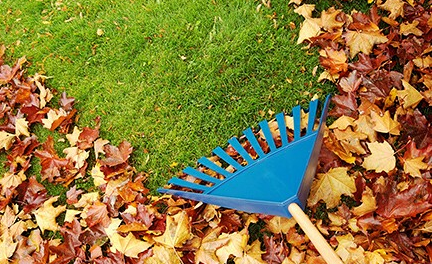
\includegraphics[angle=0,scale=4.0]{Figures/Laub/Titelfoto.png}}
\label{Titelfoto}
\end{minipage}
\end{center}

\tableofcontents


\mainmatter

\chapter{Einleitung}
Das jährliche Laubharken in Gärten oder Parks stellt eine sehr spezielle, alltagsnahe Ausprägung von allgemeinen Entsorgungsprozessen dar und eignet sich nicht zuletzt aufgrund dieses \glqq Bekanntheitsgrades\grqq{}  als didaktisches Musterbeispiel, um in die Bereiche der mathematischen Modellierung, Optimierung und Simulation einzuführen, zumal es sich in der Gesamtheit als ein recht komplexes Problem herausstellt. Schließlich ergeben sich hierbei mehrere Fragestellungen, die simultan oder sukzessiv zu lösen sind: 

\begin{itemize} 
\item Soll das zu entsorgende Laub auf viele kleine oder wenige große Laubhaufen zusammengeharkt werden? 
\item Wo sollen diese Laubhaufen gebildet werden? 
\item Von welchen Feldern soll zu welchen Laubhaufen geharkt werden? 
\item In welcher Reihenfolge sollen dabei die einzelnen Felder bearbeitet werden?
\item Welcher Aufwand ergibt sich dabei einerseits beim Harkprozess, andererseits beim Transportprozess (Abtransport der Laubhaufen mit einem Laubwagen zu einer oder zu mehreren Kompoststellen). 
\item Wie lassen sich dabei unproduktive Wege möglichst vermeiden? 
\end{itemize}

 \noindent 
Die Bestimmung von optimalen Standorten für die Laubhaufen lässt sich auch als ein spezielles Hub-Location-Problem auffassen. Somit ist es nicht verwunderlich, wenn gängige Lösungsansätze für Standortplanungsprobleme in adaptierter Form auch zur Lösung des Laubharkproblems zur Anwendung kommen.\\
\\
Einen Vorschlag für die Modellierung des Laubharkproblems findet man in \cite{kruse}. Hierbei wird ein Garten durch beliebig feine Rasterung in Matrixform gebracht, wodurch endlich viele Felder entstehen und die Grundlage für ein kombinatorisches Optimierungsmodell gegeben ist. Durch die Festlegung der Nachbarschaft dieser Felder, welche die Möglichkeiten von direkten Harkvorgängen beschreiben, ergibt sich auf kanonische Weise ein ungerichteter Graph, dessen Kantenbewertungen den zeitlichen Aufwand sowohl für den Hark- als auch für den Transportprozess angeben. Die Minimierung des Gesamtaufwandes, in den Einzelaufwände für die Teilprozesse parametrisiert eingehen, lässt sich somit als ein kombinatorisches Optimierungsproblem formulieren (Näheres hierzu siehe in Kapitel \ref{chapterProblembeschreibung}). \\
\\
\noindent Für diejenigen Leser/innen, die sich nicht so sehr für eine anschauliche und ausführliche Herleitung der Modellierung des Laubharkprozesses als ein kombinatorischen Optimierungsproblems interessieren, mag ein direkter Einstieg zum Ende von Kapitel \ref{chapterProblembeschreibung} genügen, wo das mathematische Optimierungsmodell in konzentrierter Form vorgestellt wird (Abschn. \ref{sectionFormalmodell}). \\
\\
Einige Lösungsansätze für dieses spezielle Optimierungsproblem findet man in \cite{kruse_et_al}.
Diese basieren zum Teil auf klassischen Heuristiken für kombinatorische Optimierungsprobleme und sind auf die spezielle Problematik passend zugeschnitten (hierzu siehe Kapitel \ref{chapterLösungsstrategien}).\\
\\


\chapter{Das Laubharkproblem als kombinatorisches Optimierungsproblem}
\label{chapterProblembeschreibung}

Um ein reales Laubharkproblem mit Hilfe von mathematischen 
Optimierungsverfahren einer Lösung zuführen zu können, bedarf es zunächst einer 
Abstraktion des Problems zwecks Bildung eines mathematischen Modells. 
Die Modellbildung erfolgt in mehreren Stufen. Zunächst wird ein abstraktes 
Modell für den Garten geschaffen. Anschließend werden Überlegungen zur Festlegung 
einer geeigneten Zielgröße angestellt und ein Aufwandsmodell entwickelt. Dabei wird die Relevanz von problemspezifischen Nebenbedingungen und Annahmen diskutiert.

\section{Gartenmodelle}
\label{sectionGartenmodelle}

In der folgenden Abbildung ist ein kleiner Garten skizziert. Man erkennt die 
Rasenfläche (lindgrün), den Teich (blau), das Gerätehaus (rot), die Kompoststelle
(dunkeloliv), einige Bäume (braun) und die gepflasterten Gehwege (grau).\footnote{Natürlich 
sind Rasenflächen nicht in allen Gärten rechteckig, aber diese Gegebenheit wird
die Modellierung des Gartens und die Veranschaulichung der noch zu entwickelnden 
Laubharkstrategien erleichtern; daher werde die Rechteckform o.B.d.A. angenommen.}

\begin{center}
\begin{minipage}{\linewidth}
\centering
\begin{tikzpicture}[node distance=0cm,>=stealth',bend angle=45,auto,background
rectangle/.style={fill=green!50!white}, show background rectangle]
\tikzstyle{every label}=[black]
\begin{scope}[scale=0.65, transform shape] 

\node (Baum1) [circle, xshift=3cm, yshift=0.5cm,fill=brown,minimum
height=6mm,minimum width=6mm] {};
\node (Baum2) [circle, xshift=4cm, yshift=7.5cm,fill=brown, minimum height=6mm,
minimum width=6mm] {}; 
\node (Baum3) [circle, xshift=5.5cm, yshift=4cm,fill=brown,minimum
height=6mm,minimum width=6mm] {}; 
\node (Baum4) [circle, xshift=9cm, yshift=2.7cm,fill=brown,minimum
height=6mm,minimum width=6mm] {}; 
\node (Baum5) [circle, xshift=12cm, yshift=4cm,fill=brown,minimum
height=6mm,minimum width=6mm] {}; 

\node (Gerätehaus) [rectangle,xshift=14cm, yshift=0cm,fill=red,minimum
height=25mm,minimum width=25mm] {Gerätehaus}; 
\node (Kompost) [rectangle,xshift=14.5cm,
yshift=8.5cm,fill=black!50!green,minimum height=10mm,minimum width=10mm]
{\textcolor{white}{\textbf{Kompost}}}; \node (Teich) [rectangle,xshift=8.5cm,
yshift=6cm,rounded corners,fill=blue,minimum height=27mm,minimum width=35mm]
{\textcolor{white}{\textbf{Teich}}};

\draw[-,line width=8pt,black!20!white] (6.4,0)--(12.75,0);
\draw[-,line width=8pt,black!20!white] (0,6.5)--(6.5, 6.5)--(6.5,-1); 
\draw[-,line width=8pt,black!20!white] (6.5,4.5)--(10.5,4.5)--(10.5,8.5)--(13.6,8.5);
\end{scope}

\end{tikzpicture}
\captionof{figure}{Skizze eines Gartens}
\label{HJKmlp_image_Gartenskizze}
\end{minipage}
\end{center}

 \noindent Als weitergehende Abstraktionsstufe\footnote{Als erste Abstraktionsstufe muss
 bereits die Skizzierung des Gartens angesehen werden, zumal diese schon ein
 Modell der Realität darstellt. Streng genommen wäre sogar schon ein Foto des 
 Gartens (z.B. aus der Vogelperspektive) ein Modell.} bietet sich die Rasterung 
 der Rechteckfläche an (siehe Abb.~\ref{HJKmlp_image_GartenRaster}).
 Hierbei entsteht eine Matrixform, bestehend aus $m$ Zeilen und $n$ Spalten. Die
 \textit{Felder}\label{Felder} in dieser Matrixdarstellung werden mit $(i,j)$ bezeichnet, wobei 
 $i$ und $j$ auch als \textit{Koordinaten} des Feldes bezeichnet werden 
 $(i=1,...,m,\ j=1,...,n)$.\footnote{Wie fein- bzw. grobmaschig die Rasterdarstellung sein soll, bleibt dem Modellbauer überlassen. Je grober die Rasterung angelegt wird, um so mehr 
werden die realen Konturen des Gartens verloren gehen. Es wird also die
"`Kunst"' des Modellbauers sein, die Größe $m\times n$ der Matrix so einzurichten, dass
die Laubharkstrategien, die anhand des Rastermodells getestet werden, den realen 
Ablauf eines Harkprozesses in seinen wesentlichen Grundzügen zweckdienlich 
widerspiegeln.}

\begin{center}
\begin{minipage}{\textwidth}
\centerline{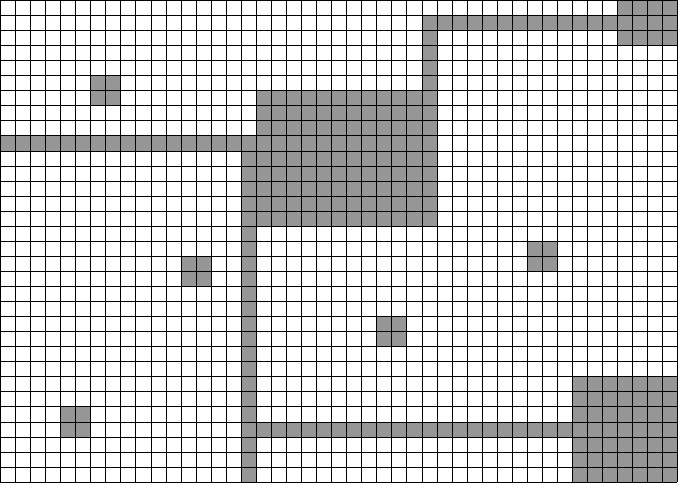
\includegraphics[angle=0,scale=0.7]{Figures/Laub/GartenRaster.jpg}}
\captionof{figure}{Gerasterte Gartendarstellung}
\label{HJKmlp_image_GartenRaster}
\end{minipage}
\end{center}

\phantom \\
\noindent Es wird sich als sehr praktisch erweisen, jedes Feld anstelle eines Koordinatenpaares 
$(i,j)$ auch durch eine natürliche Zahl $a \in \mathbb{N}$ zu beschreiben. Hierfür wird jedem Feld $(i,j)$ bijektiv die Zahl $a$ zugewiesen gemäß 

\begin{align}
a=(i-1)\cdot n+j.\label{HJKmlp_equation_Formel1}
\end{align}

\noindent Im Garten wird das Laub nun in der Regel sehr unterschiedlich auf der Rasenfläche (und den Gehwegen) verteilt liegen.\footnote{Hierbei muss von vornherein festgelegt sein, welche Felder vom Laub befreit werden sollen. Dieses sind sicherlich die Felder der Rasenfläche, können womöglich aber auch die Felder der Gehwege sein, während die Felder, die zum Teich, zum Gerätehaus und zum Baumbestand zählen, keiner Laubentfernung durch Harken unterstellt
werden sollen bzw. können.} 
Genau genommen müsste man sich jetzt die Mühe machen, in jedem relevanten Feld $(i,j)$, 
das zur Rasenfläche (oder den Gehwegen) gehört, die Anzahl der Laubblätter zu zählen und 
diese Anzahl dem Feld $(i,j)$ zuzuweisen. Eine derart genaue Laubbestandsaufnahme käme 
allerdings einer Einzelblattlese gleich, wonach sich das Laubharkproblem nicht mehr stellte. 
Daher werden die Laubmengen in den Feldern höchstens nach Augenschein geschätzt 
und registriert. Jedes Feld $a$ bekommt somit eine (wie auch immer ermittelte)
\textit{Laubmenge}\label{Laubmenge} $M(a)$ zugeordnet.\footnote{Die Laubmenge $M(a)$ für ein Feld $a=(i,j)$ wird bei Koordinatendarstellung mit $M(i,j)$ bezeichnet.} Diese
Laubmenge wird in \textit{Laubmengeneinheiten}\label{Laubmengeneinheiten} [ME] gemessen.\footnote{Hierbei könnte es sich um die Anzahl der Laubblätter oder um 100 Gramm Laub oder um diejenige Laubmenge handeln, die bei einem Harkzug mit einer normierten Harke 
(durchschnittlich) bewegt werden kann. Hierauf wird später bei der Aufwandsberechnung 
für den Harkprozess noch näher eingegangen.} Für jede Laubmenge gilt sinnvollerweise 
die Nichtnegativitätsbedingung:

\begin{align}
M(a) \geq 0.\label{HJKmlp_equation_Formel2}
\end{align}

\noindent Dabei kann die Laubmenge je nach Gutdünken des Modellbauers bzw. nach Präzision der 
Laubmengenermittlung als reelle oder als ganze Zahl zugelassen werden. Der zweite 
Fall, d.h. $M(a) \in \mathbb{N}_0$, bietet sich an, wenn zur Ermittlung der
Laubmengen feste Klassengrößen vorgegeben sind, etwa $M(a)=0$ für den Fall, dass
kein Laub im Feld $a$ vorhanden ist, und $M(a)=1, 2, 3$ usw. für den
Sachverhalt, dass die Laubmenge $M(a)$ mit einem Zug bzw. mit zwei bzw. drei
Zügen aus dem Feld $a$ in ein benachbartes Feld geharkt werden kann. Der Einfachheit halber 
soll im Folgenden vornehmlich die ganzzahlige Variante benutzt werden.\\
\\
In der Matrixdarstellung des Gartens wird nun in jedes Feld $a=(i,j)$ der Wert
der zugehörigen Laubmenge $M(a)=M(i,j)$ geschrieben (siehe
Abb.~\ref{HJKmlp_image_Gartenmatrix}), wobei die Gleichung $M(a)=0$ zwei Rückschlüsse
zulässt: Zum einen kann es ein problemrelevantes Feld sein, welches lediglich kein Laub aufweist; 
zum anderen kann es sich um ein grundsätzlich auszuschließendes Feld handeln, etwa ein Teich- oder Gerätehausfeld. Die folgende Laubmengenmatrix $M$ stellt einen mit Laub befallenen Garten dar, allerdings handelt es sich dabei um ein vereinfachtes Beispiel ($m=10, n=20$). Dabei seien die grau unterlegten Nullfelder diejenigen, die im Harkprozess auszulassen sind.

\begin{center}
\begin{minipage}{\textwidth}
\renewcommand{\arraystretch}{1.0}
\begin{table}[H]
\centering 
\begin{scriptsize}
\begin{tabular}{|>{}c|>{}c|>{}c|>{}c|>{}c|>{}c|>{}c|>{}c|>{}c|>{}c|>{}c|>{}c|>{}c|>{}c|>{}c|>{}c|>{}c|>{}c|>{}c|>{}c|}
\hline
1&2&0&3&3&2&4&3&3&2&1&2&3&4&4&3&2&1&\cellcolor{gray!50!white}0&\cellcolor{gray!50!white}0\\
\hhline{|--------------------|} 
2&2&3&2&3&2&3&3&4&3&2&3&3&5&4&4&3&1&\cellcolor{gray!50!white}0&\cellcolor{gray!50!white}0 \\
\hline
2&4&5&3&2&2&2&2&3&1&1&1&2&4&2&5&4&3&1&0 \\
\hline
3&6&\cellcolor{gray!50!white}0&4&3&2&2&2&1&\cellcolor{gray!50!white}0&\cellcolor{gray!50!white}0&\cellcolor{gray!50!white}0&\cellcolor{gray!50!white}0&2&3&6&\cellcolor{gray!50!white}0&4&2&3\\
\hline
2&5&4&4&3&5&4&3&1&\cellcolor{gray!50!white}0&\cellcolor{gray!50!white}0&\cellcolor{gray!50!white}0&\cellcolor{gray!50!white}0&1&3&6&5&3&2&2
\\
\hline
1&2&2&2&1&5&8&6&2&\cellcolor{gray!50!white}0&\cellcolor{gray!50!white}0&\cellcolor{gray!50!white}0&\cellcolor{gray!50!white}0&2&4&3&3&3&2&2
\\
\hline
1&4&4&3&2&5&\cellcolor{gray!50!white}0&7&4&2&3&4&4&5&\cellcolor{gray!50!white}0&4&\cellcolor{gray!50!white}0&\cellcolor{gray!50!white}0&\cellcolor{gray!50!white}0&\cellcolor{gray!50!white}0
\\
\hline
1&4&\cellcolor{gray!50!white}0&5&3&6&5&6&4&3&2&1&2&1&3&3&\cellcolor{gray!50!white}0&\cellcolor{gray!50!white}0&\cellcolor{gray!50!white}0&\cellcolor{gray!50!white}0 \\
\hline
1&2&3&5&2&3&3&4&2&1&1&2&2&2&2&1&\cellcolor{gray!50!white}0&\cellcolor{gray!50!white}0&\cellcolor{gray!50!white}0&\cellcolor{gray!50!white}0 \\
\hline
1&2&1&2&1&1&1&1&0&0&0&1&2&3&2&2&\cellcolor{gray!50!white}0&\cellcolor{gray!50!white}0&\cellcolor{gray!50!white}0&\cellcolor{gray!50!white}0 \\
\hline
\end{tabular}
\captionof{figure}{Beispiel für einen Garten in Matrixdarstellung}
\label{HJKmlp_image_Gartenmatrix}
\end{scriptsize} 
\end{table}
\renewcommand{\arraystretch}{1}
\end{minipage}
\end{center}

\noindent Um die Nullelemente in der Matrix $M$ bezüglich ihrer jeweiligen Bedeutung 
(laubleeres oder auszulassendes Feld) für spätere Berechnungen anhand des 
Zahlenwertes unterscheiden zu können (und nicht unter Zuhilfenahme von grafischen 
Markierungen wie etwa Schattierungen), könnte vereinbart werden, die vom 
Laubharkprozess auszuschließenden Felder mit einem negativen Wert (z.B. –1) oder 
als Blank zu identifizieren.  
\\ \\
In Anlehnung an das Harken in einem realen Garten wird der gesamte Harkprozess in 
Teilprozesse unterteilt, und zwar wird davon ausgegangen, dass die Laubmenge
$M(a)$ eines Feldes $a$ in ein benachbartes Feld $b$ geharkt wird. Bei diesem
Teilprozess werden die Laubmengen $M(a)$ und $M(b)$ verändert, und zwar
gilt:

\begin{align}
M_{neu}(b)=M_{alt}(b)+M_{alt}(a), M_{neu}(a)= 0.
\label{HJKmlp_equation_Formel3}
\end{align}

\noindent Hierbei ist allerdings noch zu vereinbaren, was unter der "`Nachbarschaft"'
zwischen Feldern\label{benachbarte Felder} konkret verstanden werden soll. Hierzu bieten sich zwei Nachbarschaftsmodelle an.\footnote{Ein weiteres interessantes Nachbarschaftsmodell wäre die Darstellung des Gartens als Wabenmuster, sodass sich auf kanonische Weise jeweils bis zu sechs Feldnachbarn ergeben. Diese Darstellungsmöglichkeit wird im Folgenden aber nicht weiter ausgeführt, zumal diese sich in die Graphenmodellen wiederfinden lässt.} 
\\ \\
Zwei Felder $a$ und $b$ heißen \textit{benachbart}, wenn gilt\footnote{Für "`Randfelder"' gelten auf kanonische Weise eingeschränkte Bedingungen.}:

\begin{align}
   a=(i,j) \wedge [b=(i,j-1) \vee b=(i,j+1) \vee b=(i-1,j) \vee
   b=(i+1,j)].\label{HJKmlp_equation_Formel4}
\end{align}

\noindent Bei dieser Variante (a) lässt sich eine Laubmenge $M(a)$ immer nur senkrecht
oder waagerecht, also in das nächste obere oder untere bzw. in das nächste linke oder 
rechte Feld harken (vgl. Abb.~\ref{HJKmlp_image_Nachbarschaftsvarianten} links). Die nächste Variante (b) lässt zudem noch diagonales Harken und somit vier weitere Möglichkeiten zu (vgl. Abb.~\ref{HJKmlp_image_Nachbarschaftsvarianten}
rechts):

\begin{equation}
   \begin{split}
      a=(i,j) & \wedge [b=(i-1,j-1) \vee b=(i-1,j) \vee b=(i-1,j+1) \\ 
	& \vee b=(i,j-1) \vee b=(i,j+1) \vee b=(i+1,j-1) \\ & \vee b=(i+1,j)  \vee b=(i+1,j+1)].
   \end{split}
   \label{HJKmlp_equation_Formel5}
\end{equation}

\begin{center}
\begin{minipage}{\linewidth}
\centering
\begin{tikzpicture}[node distance=0cm,>=stealth',bend angle=45,auto,background
rectangle/.style={fill=green!10!white}]
\tikzstyle{every label}=[black]
\begin{scope}[scale=1, transform shape] 

\node (text_a) [rectangle, xshift=5cm, yshift=2.5cm,minimum
height=3mm,minimum width=42mm] {\textcolor{black}{Variante (b)}}; 
\node (text_b) [rectangle,xshift=0cm, yshift=2.5cm,minimum height=3mm,minimum 
width=42mm] {\textcolor{black}{Variante (a)}}; 
\node (Variante_a) [rectangle,xshift=5cm, yshift=0cm,fill=gray!5!white,minimum
height=42mm,minimum width=42mm] {}; 
\node (Variante_b) [rectangle,xshift=0cm, yshift=0cm,fill=gray!5!white,minimum
height=42mm,minimum width=42mm] {}; 

\draw[-,line width=1pt,black!25!white] (-2.1,2.1)--(2.1,2.1);
\draw[-,line width=1pt,black!25!white] (-2.1,0.7)--(2.1,0.7);
\draw[-,line width=1pt,black!25!white] (-2.1,-0.7)--(2.1,-0.7);
\draw[-,line width=1pt,black!25!white] (-2.1,-2.1)--(2.1,-2.1); 

\draw[-,line width=1pt,black!25!white] (-2.1,2.1)--(-2.1,-2.1);
\draw[-,line width=1pt,black!25!white] (-0.7,2.1)--(-0.7,-2.1);
\draw[-,line width=1pt,black!25!white] (0.7,2.1)--(0.7,-2.1);
\draw[-,line width=1pt,black!25!white] (2.1,2.1)--(2.1,-2.1);

\draw[<->,line width=2pt,black] (0,1.5)--(0,-1.5);
\draw[<->,line width=2pt,black] (-1.5,0)--(1.5,0);

\draw[-,line width=1pt,black!25!white] (2.9,2.1)--(7.1,2.1);
\draw[-,line width=1pt,black!25!white] (2.9,0.7)--(7.1,0.7);
\draw[-,line width=1pt,black!25!white] (2.9,-0.7)--(7.1,-0.7);
\draw[-,line width=1pt,black!25!white] (2.9,-2.1)--(7.1,-2.1); 

\draw[-,line width=1pt,black!25!white] (2.9,2.1)--(2.9,-2.1);
\draw[-,line width=1pt,black!25!white] (4.3,2.1)--(4.3,-2.1);
\draw[-,line width=1pt,black!25!white] (5.7,2.1)--(5.7,-2.1);
\draw[-,line width=1pt,black!25!white] (7.1,2.1)--(7.1,-2.1);

\draw[<->,line width=2pt,black] (3.5,1.5)--(6.5,-1.5);
\draw[<->,line width=2pt,black] (3.5,0)--(6.5,0);
\draw[<->,line width=2pt,black] (3.5,-1.5)--(6.5,1.5);
\draw[<->,line width=2pt,black] (5,1.5)--(5,-1.5);

\end{scope}

\end{tikzpicture}
\captionof{figure}{Nachbarschaftsvarianten}
\label{HJKmlp_image_Nachbarschaftsvarianten}
\end{minipage}
\end{center}

\phantom \\
\noindent Ein in Matrixform abstrahierter Garten lässt sich anhand des Nachbarschaftsbegriffs 
auf kanonische Weise als \textit{Graph}\label{Graph} veranschaulichen. Jedes problemrelevante
Feld $a$ wird dabei als ein Knoten des Graphen aufgefasst; zwei benachbarte Felder $a$
und $b$ werden im Graph durch eine Kante $[a,b]$ verbunden. Der so entstehende
Graph werde mit $G=[V,E]$ bezeichnet, wobei $V$ die \textit{Knotenmenge}\label{Knotenmenge} und $E$ die \textit{Kantenmenge}\label{Kantenmenge} des Graphen heißen. Da in der Praxis das Harken zwischen je zwei benachbarten Feldern $a$ und $b$ grundsätzlich in beide Richtungen möglich ist, handelt es sich bei $G$ um einen ungerichteten Graph. Zudem bekommen die vom
Harkprozess auszuschließenden Felder keine Knotenzuweisung. Jeder Knoten $a \in
V$ von $G$ wird mit der Laubmenge $M(a)$ des zugehörigen Feldes $a=(i,j)$
bewertet. Somit entsteht ein knotenbewerteter Graph $G=[V,E,M]$, wobei $M:E
\rightarrow \mathbb{R}_\geq$ die \textit{Knotenbewertung}\label{Knotenbewertung} von $G$ heißt.
\\ \\
Das in Abb.~\ref{HJKmlp_image_Gartenmatrix} vorgestellte Gartenbeispiel in Matrixform
erhält je nach Nachbarschaftsvariante  die folgenden Darstellungen als Graph 
(siehe Abb.~\ref{HJKmlp_image_Nachbarschaft_a} bzw. Abb.~\ref{HJKmlp_image_Nachbarschaft_b}),
an denen unschwer zu erkennen ist, dass somit auch beliebige Gartenformen
mittels Graphen abstrahiert werden können.

\begin{center}
\begin{minipage}{\textwidth}
\centerline{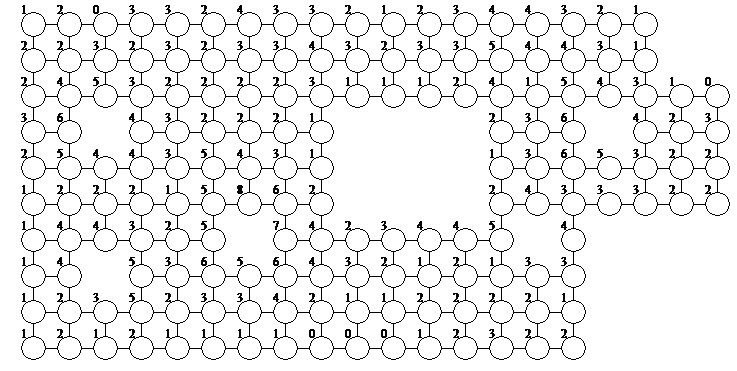
\includegraphics[angle=0,scale=0.64]{Figures/Laub/Nachbarschaftsvariante_a.jpg}}
\captionof{figure}{Graphendarstellung eines Gartens gemäß
Nachbarschaftsvariante (a)}
\label{HJKmlp_image_Nachbarschaft_a}
\end{minipage}
\end{center}

\begin{center}
\begin{minipage}{\textwidth}
\centerline{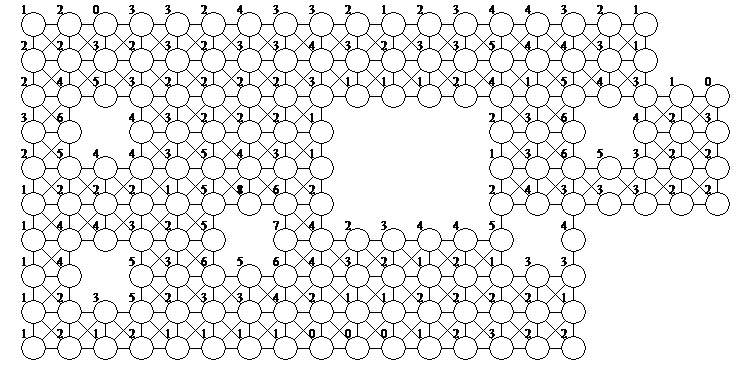
\includegraphics[angle=0,scale=0.64]{Figures/Laub/Nachbarschaftsvariante_b.jpg}}
\captionof{figure}{Graphendarstellung eines Gartens gemäß
Nachbarschaftsvariante (b)}
\label{HJKmlp_image_Nachbarschaft_b}
\end{minipage}
\end{center}
	 
\phantom \\
\noindent Zudem bietet es sich an, auch die Kanten des Graphen zu bewerten, wobei die Elemente $c_{a,b}$ der \textit{Bewertungsmatrix} $C$\label{Bewertungsmatrix} Feldabstände oder Harkaufwände zwischen benachbarten Knoten (Feldern) $a$ und $b$ wiedergeben können.\footnote{Näheres hierzu in Abschn.~\ref{sectionAufwandsberechung}} 
Die Darstellung eines Gartens als knoten- und kantenbewerteter Graph hat den beträchtlichen Vorteil, dass auszulassende Felder nicht mehr in der Knotenmenge enthalten sind. 
Zudem lässt sich aus der Bewertungsmatrix $C$ des Graphen sehr einfach eine Entfernungsmatrix\label{Entfernungsmatrix} $D$ ermitteln, mit deren Hilfe die Hark- und Transportaufwände berechnet werden können, sobald die Hark- und Transportwege bestimmt sind. 

\section{Aufwandsberechung}
\label{sectionAufwandsberechung}

\noindent Nachdem nun Matrix- und Graphenmodelle zur abstrahierten Darstellung von Gärten 
eingeführt sind, stellt sich die ebenso wichtige Frage nach der Zielgröße, an der 
die Güte eines Entsorgungsprozesses gemessen werden soll. Hier ist wieder der 
Entscheidungsträger gefragt, denn dieser legt fest, ob er ein möglichst Zeit, Wege oder Kräfte sparendes Vorgehen anstrebt. Um hierfür viele Möglichkeiten offen zu lassen, soll im Folgenden sehr allgemein von "`\textit{Zeitkosten}"'\label{Zeitkosten} gesprochen werden. Diese werden in der Dimension [ZE] für \textit{Zeitkosteneinheit}\label{Zeitkosteneinheit} gemessen. Hierbei kann es sich im konkreten Fall um Zeit [t] oder Kosten [GE] oder andere Messgrößen handeln. Es wird allerdings wichtig sein, darauf zu achten, dass alle Teilprozesse in derselben Dimension gemessen werden, sodass ein eindeutiges Gütemaß für den gesamten Entsorgungsprozess zur Verfügung steht.
\\ \\
Der gesamte Entsorgungsprozess besteht im Wesentlichen aus den drei 
Teilprozessen Harken, Aufladen und Abtransportieren des Laubes. Und so, wie 
es verschiedene Nachbarschaftsmodelle gibt, lassen sich auch verschiedene 
Ansätze zur Berechnung des jeweiligen Aufwandes dieser Teilprozesse finden. 

\subsection{Berechnung des Harkaufwandes}
\label{subsectionHarkaufwandsberechnung}

Der Harkprozess besteht aus dem Laubharken selbst, also aus Tätigkeiten, bei denen das Laub bewegt wird, aber auch aus unproduktiven Wegezeiten, die zwischen den einzelnen Harkvorgängen anfallen können. Diese werden im Folgenden getrennt voneinander betrachtet. Zunächst wird in diesem Abschnitt der eigentliche Harkprozess betrachtet; die unproduktiven Wege werden in Abschn.~\ref{subsectionWegezeitenberechnung} untersucht.\\
\\
Eine sehr einfache Berechnungsvorschrift ist es, den \textit{Harkaufwand}\label{Harkaufwand}
$HA(a,b)$ eines Teilprozesses, d.h. den Aufwand für das Harken der aktuellen Laubmenge $M^*(a)$ vom Feld $a$ in das Feld $b$, proportional zur Laubmenge anzunehmen: \label{Kru_Seite_Harkaufwandsmodell}

\begin{align}
HA(a,b) = M^*(a)\cdot \alpha_H, \alpha_H>0,
\label{Harkaufwandsformel_1}
\end{align}

\noindent wobei $\alpha_H$ als \textit{Harkaufwandsfaktor}\label{Harkaufwandsfaktor} oder kurz als \textit{Harkparameter}\label{Harkparameter} bezeichnet werden soll, welcher angibt, wie viel
Zeitkosten beim Harken einer Laubmengeneinheit [ME] von einem Feld $a$ zu 
einem benachbarten Feld $b$ entsteht. Dabei wird zunächst angenommen, dass der 
Harkparameter unabhängig von den Feldern eine konstante Größe darstellt. 
Der Parameter $\alpha_H$ hat in diesem Fall die Dimension [ZE/ME], sodass 
sich für den Harkaufwand die Dimension [ZE] ergibt. Mit $M^*(a)$ ist diejenige aktuelle Laubmenge\label{aktuelle Laubmenge} im Feld $a$ gemeint, die zum Zeitpunkt des Harkens von Feld $a$ in das Nachbarfeld $b$ vorliegt; die aktuelle Laubmenge $M^*(a)$ wird sich durch den ausgeführten Harkprozess im Allgemeinen von der initialen Laubmenge $M(a)$ unterscheiden.
\\ \\
Nach genauerer Betrachtung dieser simplen Harkaufwandsberechnung stellen 
sich allerdings erste Zweifel an deren Praxisnähe ein. Letztere lässt sich 
nämlich wohl nur unter idealisierten Voraussetzungen vertreten. Da wäre 
zunächst die Annahme der Feldunabhängigkeit zu untersuchen. Ist diese in 
der Praxis nicht gegeben, könnte allerdings der Übergang von der konstanten 
Größe $\alpha_H$ auf variable Größen $\alpha_H(a,b)$ als erste 
Verallgemeinerung der Berechnung des Harkaufwandes sinnvoll sein\footnote{Die Harkaufwandsfaktoren $\alpha_H(a,b)$ können beim Graphenmodell ohne Weiteres als Elemente der Bewertungsmatrix $C$ hinterlegt werden.}:

\begin{align}
HA(a,b) = M^*(a) \cdot \alpha_H(a,b).\label{Harkaufwandsformel_2}
\end{align}	

\noindent Somit ergibt sich (\ref{Harkaufwandsformel_1}) auf kanonische Weise als Spezialfall von
(\ref{Harkaufwandsformel_2}), wenn $\alpha_H(a,b) \equiv  \alpha_H$ für alle benachbarten Felderpaare $(a,b)$ gilt $(a \neq b)$. Zudem wird $\alpha_H(a,a)=0$ für alle Felder $a$ vereinbart.
\\ \\
Weiterhin ist die Annahme der Proportionalität zweifelhaft. Hierbei wird 
unterstellt, dass sich der Aufwand für das Harken eines Blattes bei zwei 
Blättern verdoppelt, wenn exemplarisch für die Laubmengeneinheit [ME] ein 
Laubblatt angenommen wird. Praxisnäher aber dürfte die Unterstellung sein, 
dass ein Zug mit einer Harke nur unwesentlich von der damit bewegten 
Laubmenge abhängt, insbesondere im Hinblick auf die dafür verbrauchte Zeit. 
Erst wenn die Laubmenge eine kritische Höhe überschreitet, sodass mehr als 
ein einziger Zug zum Harken nötig ist, um die Laubmenge $M^*(a)$ von Feld $a$ 
nach Feld $b$ zu bewegen, ergibt sich ein signifikanter zeitlicher Mehraufwand. 
Um diesem Umstand im Modell gerecht zu werden, bietet es sich an, 
für diese kritische Größe eine positive reelle Zahl $M_k$ einzuführen. 
Ist die aktuelle Laubmenge $M^*(a)$ kleiner oder gleich diesem kritischen Wert, 
so wird genau ein Harkzug benötigt. Andernfalls wird man mit einem Zug 
nicht auskommen, sondern wird zwei oder mehrere Harkzüge benötigen. 
Diese reelle Zahl $M_k$ soll \textit{kritische Laubharkmenge}\label{kritische Laubharkmenge} genannt werden.
\\ \\
Die Anzahl der benötigten Harkzüge bei vorliegender Laubmenge $M^*(a)$ ergibt 
sich dann als nächste größere ganze Zahl zum Quotienten $M^*(a)/M_k$, sodass 
sich der Harkaufwand gegenüber (\ref{Harkaufwandsformel_2}) folgendermaßen ändert\footnote{Hierbei sind $\lceil \rceil$ die Gaußklammern für die Aufrundung zur nächstgrößeren ganzen Zahl.}:
			
\begin{align}
HA(a,b) = \Big\lceil \frac{M^*(a)}{M_k} \Big\rceil \cdot \alpha_H(a,b).\label{Harkaufwandsformel_3}
\end{align}		
						
\noindent Man beachte nun aber, dass sich die Dimension der Harkparameter $\alpha_H$ 
bzw. $\alpha_H(a,b)$ geändert hat, zumal der Quotient $M^*(a)/M_k$ eine
dimensionslose Größe darstellt ([ME]/[ME]). Danach müsste der Parameter
$\alpha_H$ bzw. $\alpha_H(a,b)$ dieselbe Dimension wie der Harkaufwand
$HA(a,b)$ besitzen, also in Zeitkosteneinheiten [ZE] gemessen sein. Diese
Vereinbarung soll im Folgenden beibehalten werden, d.h. der Harkparameter 
$\alpha_H$ bzw. $\alpha_H(a,b)$ gibt an, wie viele Zeitkosteneinheiten 
für einen Harkzug benötigt werden, und zwar unabhängig von der Laubmenge, 
solange diese im Intervall zwischen 0 und der kritischen Laubharkmenge liegt, 
d.h. $0<M^*(a) \leq M_k$.
\\ \\
Nachdem nun mehrere Varianten zur Modellierung des Harkaufwandes 
im Nachbarschaftsfall, d.h. für das Harken von einem Feld $a$ auf 
ein Nachbarfeld $b$, vorgestellt worden sind, sollen weitergehende 
Überlegungen angestellt werden, wie sich diese Einzelaufwände für 
das Harken über mehrere Felder ($a \rightarrow b \rightarrow c \rightarrow d \rightarrow ...$) 
übertragen (lassen). Hierzu wird exemplarisch ein kleiner Ausschnitt 
(die nordwestliche Ecke) aus dem obigen Beispiel-Garten entnommen. 

\begin{center}
\begin{minipage}{\textwidth}
\centerline{
\includegraphics[angle=0,scale=0.9]{Figures/Laub/Gartenausschnitt.jpg}}
\captionof{figure}{Nordwestlicher Ausschnitt aus Abb.~\ref{HJKmlp_image_Nachbarschaft_a}}
\label{HJKmlp_image_Gartenausschnitt}
\end{minipage}
\end{center}

\phantom \\
\noindent Man nehme nun zunächst den idealisierten Fall an, dass die Laubmengen $M(a)$, 
die als Knotenbewertungen ersichtlich sind, mit der Anzahl der benötigten 
Harkzüge übereinstimmen. Es wird dabei also angenommen, dass jede Laubmenge 
$M(a)$ ein ganzzahliges Vielfaches der kritischen Laubharkmenge $M_k$ bei 
konstantem Harkaufwandsparameter $\alpha_H=1$ ist. Beispielsweise bedeutet 
$M(1,2)=2$, dass die Laubmenge aus dem Feld $a=(1,2)$ mit genau zwei Harkzügen 
auf ein benachbartes Feld $b$ zu harken ist. Somit ergibt sich $HA(a,b)=M(a)=2$.
\\ \\
Es sei nun zunächst die Aufgabe gestellt, das gesamte Laub in diesem 
verkleinerten Garten auf \textit{ein} ausgewähltes Feld zusammenzuharken, wobei
sich die Frage nach dem gesamten Harkaufwand dafür stellt. 
\\ \\
In diesem Zusammenhang stellt sich zunächst die Frage nach einer 
maximalen Laubmenge, die sich auf einem Feld "`antürmen"' lässt und 
die es alleine schon aus natürlichen "`Stabilitätsgründen"' für einen
Laubhaufen gibt. Eine solche \textit{maximale Laubmenge}\label{maximale Laubmenge} könnte für jedes Feld anders ausfallen, d.h. $M^*(a) \leq \overline{M}(a)$, oder als gemeinsame Obergrenze für alle Felder festgelegt werden, d.h. $M^*(a) \leq \overline{M}$ für alle Felder $a$. Im
Folgenden soll nur noch der einfache Fall einer gemeinsamen maximalen Laubmenge $\overline{M}$ zur Anwendung kommen. 
\\ \\
Um die obige Aufgabe erfüllen zu können (also \textit{ein} Sammelhaufen), muss 
die maximale Laubmenge hinreichend groß sein; im obigen Beispiel muss 
offensichtlich gelten: $\overline{M} \geq 29$. Andernfalls käme man mit einem
einzigen Sammelhaufen nicht aus.
\\ \\
Exemplarisch soll zunächst eine "`Harkstrategie"' angewendet werden, wie sie in 
Abb.~\ref{HJKmlp_image_Zickzack} als intuitives "`Zickzack-Harken"' skizziert ist. 

\begin{center}
\begin{minipage}{\textwidth}
\centerline{
\includegraphics[angle=0,scale=0.85]{Figures/Laub/Zickzack.jpg}}
\captionof{figure}{Zickzack-Harken (Variante 1)}
\label{HJKmlp_image_Zickzack}
\end{minipage}
\end{center}

\phantom \\
\noindent Der gesamte Harkaufwand, der sich aus den in Tab.~\ref{HJKmlp_table_ZZVariante1}
aufgelisteten Einzelaufwänden (Anzahl der Harkzüge) zusammensetzt, beträgt dabei 
124 Harkzüge.
 
\renewcommand{\arraystretch}{0.96}
\begin{table}[H]
\caption{Harkaufwand für Zickzack-Variante 1}
\label{HJKmlp_table_ZZVariante1}
\centering 
\begin{scriptsize}
\begin{tabular}{|>{}c|>{}c|}
\hline
\textbf{Harken} & \textbf{Aufwand}\\
(von \ldots nach) & (Anzahl Harkzüge)\\
\hline
(1,1) $\rightarrow$ (1,2) & 1\\
\hline
(1,2) $\rightarrow$ (1,3) & 3\\
\hline
(1,3) $\rightarrow$ (1,4) & 3\\
\hline
(1,4) $\rightarrow$ (2,4) & 6\\
\hline
(2,4) $\rightarrow$ (2,3) & 8\\
\hline
(2,3) $\rightarrow$ (2,2) & 11\\
\hline
(2,2) $\rightarrow$ (2,1) & 13\\
\hline
(2,1) $\rightarrow$ (3,1) & 15\\
\hline
(3,1) $\rightarrow$ (3,2) & 17\\
\hline
(3,2) $\rightarrow$ (3,3) & 21\\
\hline
(3,3) $\rightarrow$ (3,4) & 26\\
\hline
\textbf{Summe} & \textbf{124}\\
\hline
\end{tabular}
\end{scriptsize} 
\end{table}
\renewcommand{\arraystretch}{1}

\noindent Eine alternative "`Zickzack-Strategie"' ist in Abb.~\ref{HJKmlp_image_Zickzack2}
skizziert. Der gesamte Harkaufwand für diese Alternative beträgt 150 Harkzüge 
(vgl. Tab.~\ref{HJKmlp_table_ZZVariante2}). 

\begin{center}
\begin{minipage}{\textwidth}
\centerline{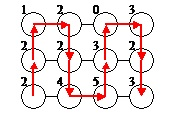
\includegraphics[angle=0,scale=0.8]{Figures/Laub/Zickzack2.jpg}}
\captionof{figure}{Zickzack-Harken (Variante 2)}
\label{HJKmlp_image_Zickzack2}
\end{minipage}
\end{center}

\renewcommand{\arraystretch}{1}
\begin{table}[H]
\caption{Harkaufwand für Zickzack-Variante 2}
\label{HJKmlp_table_ZZVariante2}
\centering 
\begin{scriptsize}
\begin{tabular}{|>{}c|>{}c|}
\hline
\textbf{Harken} & \textbf{Aufwand}\\
(von \ldots nach) & (Anzahl Harkzüge)\\
\hline
(3,1) $\rightarrow$ (2,1) & 2\\
\hline
(2,1) $\rightarrow$ (1,1) & 4\\
\hline
(1,1) $\rightarrow$ (1,2) & 5\\
\hline
(1,2) $\rightarrow$ (2,2) & 7\\
\hline
(2,2) $\rightarrow$ (3,2) & 9\\
\hline
(3,2) $\rightarrow$ (3,3) & 13\\
\hline
(3,3) $\rightarrow$ (2,3) & 18\\
\hline
(2,3) $\rightarrow$ (1,3) & 21\\
\hline
(1,3) $\rightarrow$ (1,4) & 21\\
\hline
(1,4) $\rightarrow$ (2,4) & 24\\
\hline
(2,4) $\rightarrow$ (3,4) & 26\\
\hline
\textbf{Summe}& \textbf{150}\\
\hline
\end{tabular}
\end{scriptsize} 
\end{table}
\renewcommand{\arraystretch}{1}
	 
\noindent Den beiden „Zickzack-Strategien“ wird in Abb.~\ref{HJKmlp_image_Harkvariante_3} eine weitere Harkmöglichkeit gegenübergestellt. Der gesamte Harkaufwand für diese 3. Variante beträgt 47 Harkzüge (vgl. Tab.~\ref{HJKmlp_table_Variante3}).

\begin{center}
\begin{minipage}{\textwidth}
\centerline{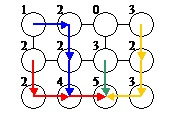
\includegraphics[angle=0,scale=0.8]{Figures/Laub/Harkvariante_3.jpg}}
\captionof{figure}{Hark-Variante 3}
\label{HJKmlp_image_Harkvariante_3}
\end{minipage}
\end{center}

\renewcommand{\arraystretch}{1}
\begin{table}[H]
\caption{Harkaufwand für Variante 3}
\label{HJKmlp_table_Variante3}
\centering 
\begin{scriptsize}
\begin{tabular}{|>{}c|>{}c|}
\hline
\textbf{Harken} & \textbf{Aufwand}\\
(von \ldots nach) & (Anzahl Harkzüge)\\
\hline
\textcolor{blue}{(1,1) $\rightarrow$ (1,2)} & 1\\
\hline
\textcolor{blue}{(1,2) $\rightarrow$ (2,2)} & 3\\
\hline
\textcolor{blue}{(2,2) $\rightarrow$ (3,2)} & 5\\
\hline
\textcolor{red}{(2,1) $\rightarrow$ (3,1)} & 2\\
\hline
\textcolor{red}{(3,1) $\rightarrow$ (3,2)} & 4\\
\hline
\textcolor{red}{(3,2) $\rightarrow$ (3,3)} & 13\\
\hline
\textcolor{green}{(2,3) $\rightarrow$ (3,3)} & 3\\
\hline
\textcolor{yellow!20!brown}{(1,4) $\rightarrow$ (2,4)} & 3\\
\hline
\textcolor{yellow!20!brown}{(2,4) $\rightarrow$ (3,4)} & 5\\
\hline
\textcolor{yellow!20!brown}{(3,4) $\rightarrow$ (3,3)} & 8\\
\hline
\textbf{Summe} & \textbf{47}\\
\hline
\end{tabular}
\end{scriptsize} 
\end{table}
\renewcommand{\arraystretch}{1}
	 	 
\noindent Anhand dieser Beispiele zeigt sich bereits sehr deutlich, dass der gesamte 
Harkaufwand entscheidend von der verwendeten "`Harkstrategie"' abhängt. 
Dabei beeinflusst nicht nur die Festlegung der Harkreihenfolge 
($a \rightarrow b \rightarrow c \rightarrow d \rightarrow ...$) den 
gesamten Harkaufwand, sondern auch die Bestimmung 
desjenigen Feldes, auf dem der durch das Zusammenharken entstehende 
\textit{Laubhaufen} errichtet werden soll.\footnote{In größeren Gärten 
bestimmen auch noch weitere Kenngrößen die Suche nach effizienten 
Laubharkstrategien, z.B. die Anzahl und die Größe der zu errichtenden 
Laubhaufen.} Zudem sei bereits an dieser Stelle angemerkt, dass bei der Harkvariante 3 unproduktive Wege während des Harkprozesses entstehen, zumal dieser mehrfach unterbrochen werden muss, und zwar jeweils beim "`Farbwechsel"' der Teilharkprozesse; diese unproduktiven Wege nehmen Zeit in Anspruch und sind somit dem produktiven Harkaufwand zuzuschlagen. Demgegenüber treten bei den Zickzack-Strategien keine solchen unproduktiven Wege auf. Näheres hierzu wird noch in Abschn.~\ref{subsectionWegezeitenberechnung} diskutiert werden.




\subsection{Darstellung der Harkprozesse durch Nachfolgerfunktionen}
\label{subsectionNachfolgerfunktion}

\noindent Um später zur Entwicklung von effizienten Strategien auf Verfahren aus der kombinatorischen Optimierung zurückgreifen zu können, wird vorweg ein Darstellungsmodell für Harkprozesse eingeführt, an welchem die Berechnung des jeweiligen Harkaufwands in einheitlicher Form vollzogen werden kann.\\

\noindent Als eine Lösung des Laubharkproblems gilt eine explizite \textit{Harkvorschrift}
in Form einer Abbildung $s:V \rightarrow V$; hierbei wird jedem Feld $a \in V$
dasjenige Nachbarfeld $b=s(a) \in V$ zugewiesen, wohin die aktuelle Laubmenge $M^*(a)$
geharkt wird. Eine anschauliche Darstellung einer Harkvorschrift ist die Tabellenform (vgl. Abb.~\ref{HJKmlp_image_Harkvariante_3}):

\renewcommand{\arraystretch}{1}
\begin{table}[H]
\caption{Beispiel einer Harkvorschrift mittels Nachfolgerfunktion}
\label{HJKmlp_table_Nachfolgerfunktion}
\centering 
% \begin{scriptsize}
\begin{tabular}{|>{}c|>{}c|>{}c|>{}c|>{}c|>{}c|>{}c|>{}c|>{}c|>{}c|>{}c|>{}c|>{}c|}
\hline
$a$ & 1&2 &3 &4 &5 & 6 & 7 & 8 & 9 & 10 & 11 & 12\\
\hline
$s(a)$ & 2 &  6 & 3 & 8 & 9 & 10 & 11 & 12 & 10 & 11 & 11 & 11\\
\hline
\end{tabular}
% \end{scriptsize} 
\end{table}
\renewcommand{\arraystretch}{1}

\noindent Die obige Tabelle besagt, dass vom Feld 1 zum Feld 2, weiter zum Feld 6, 
von dort zum Feld 10 und schließlich zum Feld 11 geharkt wird. Wegen $s(11)=11$
wird im Feld 11 ein Laubhaufen zusammengeharkt; solche Felder werden im
Folgenden \textit{Haufenfelder} oder \textit{Hubs}\label{Hub} genannt. Zudem wird vom
Feld 4 zum Feld 8, weiter zum Feld 12 und schließlich zum Haufenfeld 11 geharkt. Die Laubmenge von Feld 5 wird zum Feld 9, weiter zum Feld 10 und schließlich zum Feld 11 geharkt. Letztlich wird noch vom Feld 7 zum Feld 11 geharkt. Das Feld 3 ist wegen $s(3)=3$ ebenfalls ein Haufenfeld (Hub), allerdings wird diesem Feld kein Beitrag von einem anderen Feld zugeliefert; es stellt somit ein \textit{isoliertes Haufenfeld} dar. 
\\ \\
Damit eine Abbildung $s:V \rightarrow V$ eine Harkvorschrift darstellt, wobei ausschließlich entlang von Kanten des Graphen $G$ geharkt wird, muss für jeden Knoten $a \in V$ die \textit{Nachbarschaftsbedingung} gelten:

\begin{align}
a \neq s(a) \Rightarrow [a,s(a)] \in E.\label{HJKmlp_equation_Nachbarschaftsbedingung}
\end{align}

\noindent Man mache sich klar, dass durch eine Abbildung $s:V \rightarrow V$, die der Nachbarschaftsbedingung genügt, auf kanonische Weise ein Digraph $\vec{G}_s = \langle V,\vec{E}_s \rangle$ induziert wird, wobei die Pfeilmenge $\vec{E}_s$ aus den gerichteten Kanten $\langle a,s(a) \rangle$ mit $a \neq s(a)$ besteht. Um ein sinnvolles Harken zu gewährleisten, sollte dieser Digraph $\vec{G}_s$ zudem zyklenfrei sein. \\
\\
Eine solche Abbildung $s:V \rightarrow V$, die sowohl der Nachbarschaftsbedingung (\ref{HJKmlp_equation_Nachbarschaftsbedingung}) genügt als auch einen zyklenfreien Digraph $\vec{G}_s = \langle V,\vec{E}_s \rangle$ mit $\vec{E}_s = \{\langle a,s(a)\rangle \mid a\in V \wedge a \neq s(a)\}$\label{induzierter Teilgraph} induziert, wird im Folgenden \textit{Nachfolgerfunktion}\label{Nachfolgerfunktion} genannt.\footnote{Vgl. \cite{kruse}, S. 82.} \\
\\
Eine Harkvorschrift in Form einer Nachfolgerfunktion stellt auf kanonische Weise eine Lösung des Laubharkproblems dar, denn es werden die generierten Laubhaufen hinsichtlich der Anzahl, Lage und kumulierten Laubmenge eindeutig festgelegt. Zur Überprüfung, ob eine Abbildung $s:V \rightarrow V$ eine Nachfolgerfunktion ist, kann ein einfaches Prüfmodul implementiert werden (hierzu siehe Algorithmus \ref{Algo_Prüfung_Nachfolgerfunktion} im Anhang \ref{Anhang_Algorithmen}). \\ 
\\
Man mache sich ebenfalls klar, dass der durch eine Nachfolgerfunktion $s$ induzierte Digraph $\vec{G}_s$  eine "`inverse Baumstruktur"' besitzt, d.h. der inverse Digraph ist ein gerichteter Wald. Im obigen Beispiel ergibt sich ein gerichteter Wald mit zwei Wurzelbäumen, wobei der eine Baum den Wurzelknoten 11 und die Blätter 1, 4, 5 und 7 hat, der zweite Baum allein aus dem isolierten Knoten 3 besteht (siehe Abb.~\ref{AMMO-Heft_image_Induzierter_Digraph}).

\begin{center}
\begin{minipage}{\textwidth}
\centerline{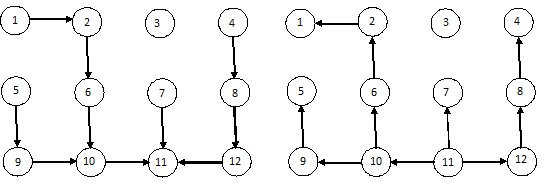
\includegraphics[angle=0,scale=1.4]{Figures/Laub/Induzierter_Digraph.png}}
\captionof{figure}{Durch Nachfolgerfunktion induzierter Digraph (links) und Wald (rechts)}
\label{AMMO-Heft_image_Induzierter_Digraph}
\end{minipage}
\end{center}

\phantom \\
\noindent Die Quellen\footnote{Quellen sind Knoten ohne Pfeileingänge in einem Digraph.} des durch eine Nachfolgerfunktion $s$ induzierten Digraphen $\vec{G}_s$ werden im Folgenden auch \textit{Harkquellen}\label{Harkquelle} genannt; sie bilden die \textit{Harkquellenmenge} \label{Harkquellenmenge} $Q(s)$ von $s$. Die Senken\footnote{Senken sind Knoten ohne Pfeilausgänge in einem Digraph.} von $\vec{G}_s$ stellen die Haufenfelder (Hubs) des Harkprozesses dar; sie bilden die \textit{Hubmenge}\label{Hubmenge} $Hub(s)$ von $s$.\\
\\
Um zu gewährleisten, dass eine Nachfolgerfunktion $s$ nicht nur im Initialzustand, sondern auch während des gesamten Harkprozesses vorgegebene Kapazitätsbeschränkungen $\overline{M}(a)$ für alle Felder $a \in V$ erfüllt, wird noch ein Zulässigkeitsbegriff eingeführt: Eine Nachfolgerfunktion $s$ wird \textit{zulässig} bzgl. $\overline{M}$ genannt, wenn bei dem durch $s$ induzierten Harkprozess beachtet wird, dass in keinem Feld $a$ und erst recht in keinem Haufenfeld mehr Laub angehäuft wird, als gemäß maximaler Laubmenge $\overline{M}(a)$ bzw. $\overline{M}$ erlaubt ist. Um diesen Sachverhalt zu formalisieren, wird zunächst zu jedem Knoten $a$ des Digraphen $\vec{G}_s$ die \textit{Erreichbarkeitsmenge}\label{Erreichbarkeitsmenge} $R(a)$ bestimmt; diese enthält alle Knoten $i \in V$, von denen aus der Knoten $a$ entlang einer Pfeilfolge in $\vec{G}_s$ erreichbar ist.\footnote{Zur Bestimmung einer Erreichbarkeitsmenge $R(a)$ dient der Algorithmus \ref{Algo_Erreichbarkeitsmengenbestimmung} im Anhang \ref{Anhang_Algorithmen}.} Die Abbildung $M^*_s:V \rightarrow \mathbb{R}_\geq$ mit der Bildungsvorschrift 
\begin{align}
M^*_s(a) := \sum\limits_{k \in R(a)}M(k) \text{ für alle Knoten } a \in V \label{Definition_Anhäufungsfunktion}
\end{align}
heißt die durch $s$ induzierte \textit{Anhäufungsfunktion}\label{Anhäufungsfunktion}. Eine Nachfolgerfunktion $s$ heißt dann \textit{zulässig} bzgl. $\overline{M}$, wenn gilt\footnote{Für eine Zulässigkeitsprüfung einer Nachfolgerfunktion dient der Algorithmus \ref{Algo_Zulässigkeitsprüfung} im Anhang \ref{Anhang_Algorithmen}.}:
\begin{align}
M^*_s(a) \leq \overline{M}(a) \text{ für alle Knoten } a \in V. \label{Formel_Zulässigkeit_Nachfolgerfunktion}
\end{align}

\noindent Es ist leicht einzusehen, dass im konstanten Falle (d.h. $\overline{M}(a)=\overline{M}$ für alle $a \in V$) die Zulässigkeitsprüfung allein auf die Hubs $a \in Hub(s)$ eingeschränkt werden kann, zumal sich daraus die Zulässigkeit für alle Knoten ergibt. Umgekehrt (d.h. $\overline{M}(a)$ nicht konstant) kann es Fälle geben, dass die Bedingung (\ref{Formel_Zulässigkeit_Nachfolgerfunktion}) zwar für alle Hubs, nicht aber für alle sonstigen Knoten gelten muss. \\ 
\\
Zur effizienten Bestimmung des Harkaufwandes\footnote{Man beachte, dass hier zunächst der reine Harkaufwand ohne Berücksichtigung von unproduktiven Wegen gemeint ist.} anhand von (zulässigen) Nachfolgerfunktionen wird eine einfache Rechenprozedur benutzt\footnote{Hierzu siehe Algorithmus \ref{Algo_Bestimmung_Harkaufwand} im Anhang \ref{Anhang_Algorithmen}}: 
Zu gegebener (zulässiger) Nachfolgerfunktion $s$ eines Graphen $G=[V,E]$ wird die Anhäufungsfunktion $M^*_s$ ermittelt. Danach wird zu jedem Nicht-Hub $a \in V\setminus Hub(s)$ der Harkaufwand $HA(a,s(a))$ gemäß einer der Harkaufwandsformeln (\ref{Harkaufwandsformel_1}) - (\ref{Harkaufwandsformel_3}) bestimmt. Abschließend werden die Einzelaufwände aufsummiert: 

\begin{align}
HA_{\Sigma}(s) = \sum_{a \in V\setminus Hub(s)}{HA(a,s(a))}. \label{Formel_Harkaufwandsumme}
\end{align}

\noindent Für die Berechnung des Harkaufwandes einer Harkvorschrift ist die Bestimmung 
derjenigen Felder relevant, von denen aus der jeweils nächste Harkzug gemacht werden soll. 
Solche Felder sollen als \textit{aktuelle Harkfelder} bezeichnet werden. Ein aktuelles Harkfeld
zeichnet sich im dafür erstellten Algorithmus\footnote{Hierzu siehe Algorithmus \ref{Algo_Bestimmung_Harkaufwand} im Anhang \ref{Anhang_Algorithmen}.} dadurch aus, dass sämtliche Vorgänger im Verlaufe des Verfahrens bereits leer geharkt worden sind.\footnote{Diese Vorgehensweise entspricht dem Prinzip des sukkzessiven Abpflückens eines 
gerichteten Baumes mit dem Hubknoten als Wurzel bzw. dem inversen Vorgehen bei einer topologischen Sortierung von zyklenfreien Digraphen. Allerdings bleibt anzumerken, dass bei dieser Harkaufwandberechnung die Zeitkosten für die unproduktiven Wege zwischen den einzelnen Feldern, insbesondere beim Wechsel von Teilharkprozessen, noch unberücksichtigt bleiben. Auf eine entsprechende Ergänzung der Harkaufwandberechnung durch Einbeziehung dieser Wegaufwände wird auf den folgenden Abschn.~\ref{subsectionWegezeitenberechnung} verwiesen.} 
\\ \\
Beispielsweise ergibt sich für die obige Nachfolgerfunktion $s$ (vgl.
Tab.~\ref{HJKmlp_table_Nachfolgerfunktion}) ein Harkaufwand $HA_\Sigma (s)$ gemäß
(\ref{Harkaufwandsformel_1}) mit $\alpha_H=1$ von 47 ZE.
Demgegenüber ergibt sich ein Harkaufwand von 124 ZE, falls der gemäß
Nachfolgerfunktion $s^*$ induzierte Harkprozess durchgeführt wird (vgl.
Tab.~\ref{HJKmlp_table_AlternativeNachfolgerfunktion}).

\renewcommand{\arraystretch}{0.8}
\begin{table}[H]
\caption{Beispiel einer alternativen Nachfolgerfunktion}
\label{HJKmlp_table_AlternativeNachfolgerfunktion}
\centering 
% \begin{scriptsize}
\begin{tabular}{|>{}c|>{}c|>{}c|>{}c|>{}c|>{}c|>{}c|>{}c|>{}c|>{}c|>{}c|>{}c|>{}c|}
\hline
$a$ & 1&2 &3 &4 &5 & 6 & 7 & 8 & 9 & 10 & 11 & 12\\
\hline
$s^*(a)$ & 2 &  3 & 4 & 8 & 9 & 5 & 6 & 7 & 10 & 11 & 12 & 12\\
\hline
\end{tabular}
% \end{scriptsize} 
\end{table}
\renewcommand{\arraystretch}{1}

\noindent Beide Harkprozesse erzeugen jeweils \textit{einen} Laubhaufen mit einer
kumulierten Laubmenge 29 ME, allerdings an verschiedenen Stellen (Feld 11 bzw. 12 ist das jeweilige Hub). Entsprechend können sich die jeweils anschließenden Transportprozesse in ihren Transportaufwänden unterscheiden, ebenso die unproduktiven Wege. An diesem Beispiel wird deutlich, dass bei festgelegter Berechnungsgrundlage jeder vorgegebenen Nachfolgerfunktion $s$ der kumulierte Harkaufwand $HA_\Sigma (s)$ zugewiesen werden kann. \\
\\
In folgender Tabelle sind einige verschiedene Nachfolgerfunktionen aufgelistet.
Es handelt sich dabei allerdings um solche "`Spezialfälle"', bei denen stets
\textit{genau ein} Laubhaufen erzeugt wird. 

\renewcommand{\arraystretch}{0.75}
\begin{table}[H]
\caption{Ausgewählte Nachfolgerfunktionen mit zugehörigem Harkaufwand}
\label{HJKmlp_table_AuswahlNachfolgerfunktionen}
\centering 
% \begin{scriptsize}
\begin{tabular}{|>{}c|>{}c|>{}c|>{}c|>{}c|>{}c|>{}c|>{}c|>{}c|>{}c|>{}c|>{}c|>{}c|>{}c|}
\hline
$a$ & 1&2 &3 &4 &5 & 6 & 7 & 8 & 9 & 10 & 11 & 12 & $HA_\Sigma (s_i)$\\
\hline
$s_1(a)$ & 2 & 6 & 3 & 8 & 9 & 10 & 11 & 12 & 10 & 11 & 11 & 11 & 47 \\
$s_2(a)$ & 2 & 3 & 4 & 8 & 9 &  5 &  6 &  7 & 10 & 11 & 12 & 12 &124 \\
$s_3(a)$ & 2 & 3 & 4 & 4 & 1 &  2 &  3 &  4 &  5 &  6 &  7 &  8 & 76 \\
$s_4(a)$ & 2 & 3 & 4 & 4 & 6 &  7 &  8 &  4 & 10 & 11 & 12 &  8 & 76 \\
$s_5(a)$ & 2 & 6 & 3 & 8 & 6 &  7 &  7 &  7 &  5 & 11 &  7 &  8 & \textcolor{red}{\textbf{46}} \\
$s_6(a)$ & 5 & 6 & 7 & 8 & 6 & 10 & 11 &  7 & 10 & 10 & 10 & 11 & \textcolor{red}{\textbf{46}}\\
$s_7(a)$ & 5 & 6 & 7 & 8 & 6 &  7 &  8 &  8 &  5 &  6 &  7 &  8 & 59 \\
$s_8(a)$ & 2 & 3 & 4 & 4 & 6 &  7 &  8 &  4 &  5 &  6 &  7 &  8 & 76 \\
\hline
\end{tabular}
% \end{scriptsize} 
\end{table}
\renewcommand{\arraystretch}{1}

\noindent Es dürfte unverkennbar sein, dass die Anzahl der verschiedenen Nachfolgerfunktionen, insbesondere bei freier Wahl der Laubhaufenanzahl, schon bei "`kleinen"' Graphen sehr groß ausfällt und mit der Größe des Graphen exponentiell anwächst. Somit besteht eine komplexe Aufgabe im Wesentlichen darin, durch geeignete Harkstrategien zulässige Nachfolgerfunktionen zu generieren und ausgehend von einer zulässigen Nachfolgerfunktion bessere Nachfolgerfunktionen in der "`Nachbarschaft"' zu finden, um damit das Laubharkproblem schrittweise zu lösen.





\subsection{Berechnung von unproduktiven Wegezeiten}
\label{subsectionWegezeitenberechnung}

\noindent Es ist offensichtlich, dass durch die Nachfolgerfunktion $s$ zwar einzelne Harkschritte und auch die grundsätzliche "`Harkstruktur"' (Anzahl und Lage der Haufenfelder mit kumulierter Laubmenge) festgelegt werden, aber der gesamte Harkvorgang dennoch nicht eindeutig beschrieben wird, weil die Reihenfolge der einzelnen Harkschritte dadurch noch nicht festgelegt ist. Die folgende Darstellung der Nachfolgerfunktion $s$ (vgl. Tab. \ref{table_Beispiel_Nachfolgerfunktion}) lässt offen, in welchem Feld der Harkprozess beginnen soll, wie nach einem Harkschritt $a \rightarrow s(a)$ fortgesetzt werden soll, insbesondere dann, wenn $s(a)$ noch Vorgängerfelder hat, die nicht leer geharkt sind, oder $s(a)$ ein Haufenfeld darstellt.

\renewcommand{\arraystretch}{1}
\begin{table}[H]
\caption{Beispiel einer Nachfolgerfunktion}
\label{table_Beispiel_Nachfolgerfunktion}
\centering 
% \begin{scriptsize}
\begin{tabular}{|>{}c|>{}c|>{}c|>{}c|>{}c|>{}c|>{}c|>{}c|>{}c|>{}c|}
\hline
$a$ & 1&2 &3 &4 &5 & 6 & 7 & 8 & 9\\
\hline
$s(a)$ & 4 &  5 & 6 & 5 & 8 & 5 & 7 & 7 & 8\\
\hline
\end{tabular}
% \end{scriptsize} 
\end{table}
\renewcommand{\arraystretch}{1}

\begin{center}
\begin{minipage}{\textwidth}
\centerline{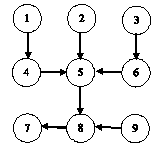
\includegraphics[angle=0,scale=1.1]{Figures/Laub/Digraph_zur_Nachfolgerfunktion.png}}
\captionof{figure}{Digraph $\vec{G_s}$ zur Nachfolgerfunktion $s$}
\label{Digraph_zur_Nachfolgerfunktion}
\end{minipage}
\end{center}

\noindent Unter Beachtung des effizienten Harkprinzips, dass nur von Feldern geharkt werden sollte, deren Vorgängerfelder bereits leer geharkt sind, wird folgerichtig mit einer Harkquelle begonnen, und bei jeder zwangsläufigen Unterbrechung des produktiven Harkprozesses wird wieder bei einer noch nicht einbezogenen Harkquelle angesetzt. Für das obige Beispiel ergeben sich anhand der vier vorhandenen Harkquellen\footnote{Die Menge der Harkquellen ist $Q(s)=\{1,2,3,9\}$; vgl. Abb. \ref{Digraph_zur_Nachfolgerfunktion}.} $4!=24$ Möglichkeiten für effiziente Harkreihenfolgen.\footnote{Man beachte, dass alle diese Harkreihenfolgen denselben Harkaufwand $HA_{\Sigma}(s)$ hervorrufen.} In der folgenden Darstellung werden exemplarisch nur die vom Startknoten $1$ ausgehenden Harkreihenfolgen aufgeführt; dabei werden produktive Harkschritte durch $\rightarrow$ und unproduktive Wege durch $\textcolor{red}{\Rightarrow}$ gekennzeichnet:\\

\noindent 
\phantom \qquad Nr. 1:\quad $1\rightarrow4\rightarrow5\textcolor{red}{\Rightarrow}
2\rightarrow5\textcolor{red}{\Rightarrow}
3\rightarrow6\rightarrow5\rightarrow8\textcolor{red}{\Rightarrow}
9\rightarrow8\rightarrow 7$ \\
\phantom \qquad Nr. 2:\quad $1\rightarrow4\rightarrow5\textcolor{red}{\Rightarrow}
2\rightarrow5\textcolor{red}{\Rightarrow}
9\rightarrow8\textcolor{red}{\Rightarrow}
3\rightarrow6\rightarrow5\rightarrow8\rightarrow7$ \\
\phantom \qquad Nr. 3:\quad $1\rightarrow4\rightarrow5\textcolor{red}{\Rightarrow}
3\rightarrow6\rightarrow5\textcolor{red}{\Rightarrow}
2\rightarrow5\rightarrow8\textcolor{red}{\Rightarrow}
9\rightarrow8\rightarrow7$ \\
\phantom \qquad Nr. 4:\quad $1\rightarrow4\rightarrow5\textcolor{red}{\Rightarrow}
3\rightarrow6\rightarrow5\textcolor{red}{\Rightarrow}
9\rightarrow8\textcolor{red}{\Rightarrow}
2\rightarrow5\rightarrow8\rightarrow7$ \\
\phantom \qquad Nr. 5:\quad $1\rightarrow4\rightarrow5\textcolor{red}{\Rightarrow}
9\rightarrow8\textcolor{red}{\Rightarrow}
2\rightarrow5\textcolor{red}{\Rightarrow}
3\rightarrow6\rightarrow5\rightarrow8\rightarrow7$ \\
\phantom \qquad Nr. 6:\quad $1\rightarrow4\rightarrow5\textcolor{red}{\Rightarrow}
9\rightarrow8\textcolor{red}{\Rightarrow}
3\rightarrow6\rightarrow5\textcolor{red}{\Rightarrow}
2\rightarrow5\rightarrow8\rightarrow7$ \\

\noindent Wird eine Entfernungsmatrix $D = (d_{ij})_{i,j=1,\dots,9}$ gemäß Manhattan-Metrik zu Grunde gelegt, ergeben sich für die obigen sechs Reihenfolgemöglichkeiten unterschiedliche Gesamtlängen für unproduktive Wege, wobei in diesem Beispiel der Einfachheit halber für die Kantenbewertungen $c_{ij}\equiv 1$ angenommen wird:\\

\noindent 
\phantom \qquad Nr. 1:\quad $d_{52} + d_{53} + d_{89} = \textbf{\textcolor{red}{4}}$ \\
\phantom \qquad Nr. 2:\quad $d_{52} + d_{59} + d_{83} = 6$ \\
\phantom \qquad Nr. 3:\quad $d_{53} + d_{52} + d_{89} = \textbf{\textcolor{red}{4}}$ \\
\phantom \qquad Nr. 4:\quad $d_{53} + d_{59} + d_{82} = 6$ \\
\phantom \qquad Nr. 5:\quad $d_{59} + d_{82} + d_{53} = 6$ \\
\phantom \qquad Nr. 6:\quad $d_{59} + d_{83} + d_{52} = 6$ \\

\noindent Somit ist die Minimierung des Aufwandes für unproduktive Wege bei einem durch eine Nachfolgerfunktion $s$ beschriebenen Harkprozess auf die Bestimmung einer optimalen Harkquellenreihenfolge zurückgeführt. Es hat sich gezeigt \cite{felker}, dass bei der Bestimmung einer "`guten"' Harkquellenreihenfolge das Greedy-Verfahren "`Nächster Nachfolger"' effiziente Lösungen anbietet. Hiernach wird ausgehend von einem beliebigen Startknoten $a \in V$ die nächstgelegene Harkquelle $k$ bestimmt:\footnote{Falls der Startknoten $a$ selbst eine Harkquelle ist, gilt $k = a$ wegen $d_{aa} = 0$.}

\begin{align}
\text{Wähle } k \in Q(s) \text{ mit } d_{ak} = \min\{d_{aj} \mid j \in Q(s)\}.
\end{align}	

\noindent Nach diesem Prinzip wird jede weitere Harkquelle bestimmt, sobald der produktive Harkprozess unterbrochen werden muss, weil der jeweilige aktuelle Knoten $a_i$ ein Hub ist oder Vorgängerknoten besitzt, die noch nicht leer geharkt sind. Dabei wird jede Harkquelle genau einmal in Anspruch genommen.\footnote{Die Mächtigkeit der durch $s$ induzierten Harkquellenmenge $Q(s)$ werde mit $Q := |Q(s)|$ bezeichnet.} Entsprechend der ermittelten Reihenfolge der Harkquellen $q_1, q_2, \dots, q_Q$ werden die Entfernungen zwischen dem jeweils aktuellen Knoten $a_{i-1}$ und der jeweils neuen Harkquelle $q_i$ kumuliert, beginnend mit einem Startknoten $a_0$:\footnote{Hierzu siehe Algorithmus \ref{Algo_unproduktive_Wege} im Anhang \ref{Anhang_Algorithmen}.} 
 
\begin{align}
W(s) = \sum_{i=1}^{Q} d_{a_{i-1},q_i}.
\label{Wegeaufwandsformel_1}
\end{align}	

\noindent Die Gesamtlänge $W(s)$ aller unproduktiven Wege $a_{i-1} \textcolor{red}{\Rightarrow} q_i \text{ für } i=1,\dots,Q$ werden noch mit einem \textit{Wegeaufwandsfaktor}\label{Wegeaufwandsfaktor} $\alpha_W$ gewichtet: 

\begin{align}
WA_{\Sigma}(s) = \alpha_W \cdot W(s) = \alpha_W \cdot \sum_{i=1}^{Q} d_{a_{i-1},q_i}.
\label{Wegeaufwandsformel_2}
\end{align}	

\noindent Der Wegeaufwandsfaktor $\alpha_W$ hat die Dimension "`Zeitkosteneinheit pro Längeneinheit"' $[ZE/LE]$, wenn die Enfernungen $d_{ij}$ bzw. die Kantenbewertungen $c_{ij}$ nach Längeneinheiten [LE] gemessen werden. Als Verallgemeinerung eines konstanten Faktors $\alpha_W$ können auch von den jeweiligen Entfernungen $d_{ij}$ abhängige Wegeaufwandsfaktoren $\alpha_W(i,j)$ eingeführt werden; dann ändert sich die Formel (\ref{Wegeaufwandsformel_2}) in 

\begin{align}
WA_{\Sigma}(s) = \sum_{i=1}^{Q}  \alpha_W(a_{i-1},q_i) \cdot d_{a_{i-1},q_i}.
\label{Wegeaufwandsformel_3}
\end{align}	

\noindent Um die Berechnung des unproduktiven Wegeaufwandes einerseits und gleichzeitig auch des produktiven Harkaufwandes gemäß (\ref{Formel_Harkaufwandsumme}) andererseits aus der tabellarischen Darstellung einer Nachfolgerfunktion $s$ unmittelbar "`ablesbar"' zu machen, wird die Nachfolgerfunktion $s$ mittels einer Permutation $\pi : V \leftrightarrow V$ ausgerichtet\label{Ausrichtung}, indem der Wert $\pi(a)$ angibt, in welcher Spalte der neu ausgerichteten Tabelle das Paar $\begin{vmatrix} a\\s(a) \end{vmatrix}$ positioniert wird. Der durch $\pi$ hervorgerufene Spaltentausch beginnt mit dem Knoten $a_1$, bei dem der Harkprozess beginnen soll, d.h. $\pi(a_1) = 1$. Danach wird vom jeweils aktuellen Knoten $a_i$ gemäß $s$ zum Knoten $s(a_i)$ geharkt, wenn $a_i$ weder Haufenfeld ist noch nichtleere Vorgängerknoten besitzt; dabei wird $\pi(a_i)=i$ gesetzt und $a_{i+1}=s(a_i)$ als nächster aktuelle Knoten betrachtet. Umgekehrt wird im Falle einer Harkunterbrechung eine jeweils neue Harkquelle $q \in Q(s)$ als nächster aktueller Knoten gewählt, d.h. $a_{i+1} = q$. \\
\\
In der folgenden Tabelle ist die Nachfolgerfunktion $s$ aus Tab. \ref{table_Beispiel_Nachfolgerfunktion} an der obigen Reihenfolgemöglichkeit Nr. 3 ausgerichtet. 

\renewcommand{\arraystretch}{1}
\begin{table}[H]
\caption{Beispiel einer ausgerichteten Nachfolgerfunktion}
\label{table_Beispiel_ausgerichtete_Nachfolgerfunktion}
\centering 
% \begin{scriptsize}
\begin{tabular}{|>{}c|>{}c|>{}c|>{}c|>{}c|>{}c|>{}c|>{}c|>{}c|>{}c|}
\hline
$\pi(a)$ &1 &2 &3 &4 &5 &6 &7 &8 &9\\
\hline
$a$     &1 &4 &3 &6 &2 &5 &9 &8 &7\\
\hline
$s(a)$ &4 &5 &6 &5 &5 &8 &8 &7 &7\\
\hline
\end{tabular}
% \end{scriptsize} 
\end{table}
\renewcommand{\arraystretch}{1}

\noindent Anhand dieser Tabelle lässt sich die Harkaufwandsberechnung sowohl der produktiven Harkschritte ($\bf{\downarrow}$) als auch der unproduktiven Wege ($\textcolor{red}{\bf{\nearrow}}$) einfach ablesen, wobei durch $\textcolor{green!80!black}{\bf{\nearrow}}$ und $\textcolor{green!80!black}{\bf{\downarrow}}$ bewertungsfreie Reihenfolgefortsetzungen angedeutet werden\footnote{Zur Ausrichtung einer Nachfolgerfunktion dient Algorithmus \ref{Algo_Ausrichtung_Nachfolgerfunktion} im Anhang \ref{Anhang_Algorithmen}.}:

\renewcommand{\arraystretch}{1}
\begin{table}[H]
\caption{Auswertung einer ausgerichteten Nachfolgerfunktion}
\label{table_Auswertung_ausgerichtete_Nachfolgerfunktion}
\centering 
\begin{tabular}{|>{}c|>{}c|>{}c|>{}c|>{}c|>{}c|>{}c|>{}c|>{}c|>{}c|}
\hline
$a$ &1 &4 &3 &6 &2 &5 &9 &8 &7\\
&$\bf{\downarrow} \textcolor{green!80!black}{\bf{\nearrow}}$ 
&$\bf{\downarrow} \textcolor{red}{\bf{\nearrow}}$ 
&$\bf{\downarrow} \textcolor{green!80!black}{\bf{\nearrow}}$ 
&$\bf{\downarrow} \textcolor{red}{\bf{\nearrow}}$ 
&$\bf{\downarrow} \textcolor{green!80!black}{\bf{\nearrow}}$ 
&$\bf{\downarrow} \textcolor{red}{\bf{\nearrow}}$ 
&$\bf{\downarrow} \textcolor{green!80!black}{\bf{\nearrow}}$ 
&$\bf{\downarrow} \textcolor{green!80!black}{\bf{\nearrow}}$
& $\textcolor{green!80!black}{\bf{\downarrow}}$\\
$s(a)$ &4 &5 &6 &5 &5 &8 &8 &7 &7\\
\hline
\end{tabular}
\end{table}
\renewcommand{\arraystretch}{1}

\noindent Entlang dieser Zickzack-Reihenfolge werden bei jedem schwarzen Pfeil $\downarrow$ die produktiven Harkaufwände $HA(a,s(a))$ mit $a\neq s(a)$ und bei jedem rotem Pfeil $\textcolor{red}{\bf{\nearrow}}$ die unproduktiven Wegeaufwände $\alpha_W\cdot d_{s(\pi^{-1}(i)),\pi^{-1}(i+1)}, i=1,\dots,n-1,$ kumuliert. An obigem Beispiel ergibt sich die folgende Rechnung\footnote{Zur simultanen Berechnung von Hark- \underline{und} Wegeaufwänden anhand einer ausgerichteten Nachfolgerfunktion dient Algorithmus \ref{Algo_Berechnung_von_HA_und_HW} im Anhang \ref{Anhang_Algorithmen}.}:

\begin{align*}
&HA(1,4) + HA(4,5) \text{ } \textcolor{red}{+ \text{ } \alpha_W(5,3)\cdot d_{5,3}} + HA(3,6) + HA(6,5) \text{ } \textcolor{red}{+ \text{ } \alpha_W(5,2)\cdot d_{5,2}} \\&+ HA(2,5) + HA(5,8) \text{ } \textcolor{red}{+ \text{ } \alpha_W(8,9)\cdot d_{8,9}} + HA(9,8) + HA(8,7).
\end{align*}	



\subsection{Berechnung des Transportaufwandes}
\label{subsectionTransportaufwandsberechnung}

\noindent Für das Aufwandsmodell des gesamten Laubharkproblems wird 
nun noch der Transportprozess einbezogen. Hierbei spielen zurückzulegende 
Transportwege zwischen den Hubs und dem Kompostfeld\label{Kompostfeld} $K$ die entscheidende Rolle.\footnote{Zur Einbeziehung des Kompostfeldes in das Graphenmodell gibt es grundsätzlich zwei Möglichkeiten: Das Kompostfeld ist ein bestimmter Knoten des Graphen ($K \in V$) oder ein zusätzlicher Knoten ($V^* = V\cup \{K\}$), allerdings jeweils mit hinreichend großer Aufnahmekapazität ($\overline{M}(K)=\infty$). Im Folgenden wird o.B.d.A. die erste Möglichkeit verfolgt.}\\
\\
Ausgehend von einer Nachfolgerfunktion $s$ sei die Hubmenge $Hub(s)$ ermittelt\footnote{Vgl. Algorithmus \ref{Algo_Prüfung_Nachfolgerfunktion}.} und ein Kompostfeld $K \in V$ vorgegeben. Die Entfernungen zwischen allen Hubs $h \in Hub(s)$ untereinander und zum Kompostfeld $K$ liegen in einer Teilmatrix $D^*=(d^*_{hk})_{h,k \in Hub(s)\cup \{K\}}$ der Entfernungsmatrix $D=(d_{ij})_{i,j \in V}$ vor. Alle Entfernungen haben die Dimension [LE] (Längeneinheit).\\
\\
Der Transportaufwand ließe sich dann proportional zu den zurückgelegten 
Weglängen bestimmen. Bei einer Pendeltour zwischen dem Kompostfeld $K$ und 
einem Hub $h$ ergibt sich im einfachsten Fall der Transportaufwand

\begin{align}
TA(h) = 2 \cdot d^*_{h,K} \cdot \alpha_T,
\label{Transportaufwandsformel_1}
\end{align}		
\noindent wobei $\alpha_T$ als \textit{Transportaufwandsfaktor}\label{Transportaufwandsfaktor} oder kurz als
\textit{Transportparameter} bezeichnet werden soll. Der Faktor $\alpha_T$ 
hat in diesem Fall die Dimension [ZE/LE], sodass sich für den 
Transportaufwand $TA(h)$ die Dimension [ZE] ergibt.
\\ \\
Allerdings können auch noch zusätzliche Aufwände eingerechnet werden, 
etwa die von der Laubmenge abhängige Auflade- und Abladezeit (\textit{variabler Ladeaufwand}\label{variabler Ladeaufwand}) oder ein 
fixer Zeitaufwand (etwa für das Vorbereiten zum Aufladen oder zum Abladen), 
welcher unabhängig von der Entfernung und der Laubmenge ist (\textit{fixer Ladeaufwand}\label{fixer Ladeaufwand}): 

\begin{align}
TA(h) = 2 \cdot d^*_{h,K} \cdot \alpha_T + \gamma \cdot M^*_s(h) + \sigma.\label{Transportaufwandsformel_2}
\end{align}

\noindent Hierbei geht der Parameter $\gamma$ in den variablen Aufwandsanteil für das 
jeweilige Auf- und Abladen der Laubmenge $M^*(h)$ ein und hat die Dimension [ZE/ME], während die Konstante $\sigma$ für den fixen Aufwandsanteil steht und die Dimension [ZE] hat.\footnote{Eine Abhängigkeit der Parameter $\gamma$ und $\sigma$ von den Hubfeldern $h$ als mögliche Verallgemeinerung, also $\gamma(h)$ und $\sigma(h)$, wird hier nicht weiter betrachtet. Es sei allerdings darauf hingewiesen, dass bei der späteren Aufsummierung der einzelnen Transportaufwände $TA(s)$ über alle Hubs (siehe (\ref{Transportaufwandsformel_5})) 
ein konstanter Parameter $\gamma$ keinen maßgeblichen Einfluss auf die Lösungsgüte einer Harkstrategie (bzw. der dadurch erzeugten Nachfolgerfunktion $s$) ausübt, wohl aber ein konstanter Parameter $\sigma$, da die Anzahl der durch $s$ induzierten Hubs hierbei eine Rolle spielt.}
\\ \\
Bislang wird unterstellt, dass die gesamte Laubmenge $M^*(h)$, die vom Hub $h$ 
abgeholt wird, auch komplett vom Transportmittel (Laubwagen oder Schubkarre) aufgenommen 
werden kann. Allerdings kann es vorkommen, dass die vom Hub $h$ 
abzuholende Laubmenge das \textit{maximale Ladevolumen}\label{Ladevolumen}
$\overline{T}$ der Schubkarre überschreitet. In diesem Falle sind mehrere
Pendeltouren nötig, um das Hub $h$ vom Laubhaufen zu befreien. Entsprechend
ändert sich der Transportaufwand für die Laubentsorgung des Haufenfeldes $h$:

\begin{align}
TA(h) = \Big\lceil \frac{M^*_s(h)}{\overline{T}} \Big\rceil \cdot 2 \cdot d^*_{h,K} \cdot \alpha_T
\label{Transportaufwandsformel_3}
\end{align}

\noindent bzw. 

\begin{align}
TA(h) = \Big\lceil \frac{M^*_s(h)}{\overline{T}} \Big\rceil  \cdot 2 \cdot d^*_{h,K} \cdot \alpha_T +
\gamma \cdot M^*_s(h) + \Big\lceil \frac{M^*_s(h)}{\overline{T}} \Big\rceil \cdot \sigma.\label{Transportaufwandsformel_4}
\end{align}

\noindent Liegen mehrere Laubhaufen zum Abholen bereit, ergibt sich der gesamte 
Transportaufwand als die Summe aller Pendeltouren zu allen Hubs (bzgl. Nachfolgerfunktion $s$):

\begin{align}
TA_\Sigma(s) = \sum_{h \in Hub(s)} TA(h).
\label{Transportaufwandsformel_5}
\end{align}

\noindent Etwas komplizierter wird die Transportaufwandsberechnung dann, wenn 
zusätzlich zu den Pendeltouren auch Sammeltouren in Frage kommen. 
Dies hat allerdings nur dann einen Sinn, wenn die auf einer Sammeltour 
angefahrenen Hubs in ihrer Laubmengensumme das maximale
Ladevolumen $\overline{T}$ nicht überschreiten. Im Folgenden wird also davon
ausgegangen, dass nur Sammeltouren $K \rightarrow h_1 \rightarrow h_2
\rightarrow \ldots \rightarrow h_P \rightarrow K$ betrachtet werden, 
für die gilt:

\begin{align}
\sum_{p=1,\ldots,P-1}{M^{**}_s(h_p)}< \overline{T},
\label{Sammeltourbedingung}
\end{align}

\noindent wobei mit $M^{**}_s(h_p)$ die nach entsprechend vielen Pendeltouren verbleibende Laubrestmenge\label{Laubrestmenge} beim Hub $h_p$ gemeint ist. Hiermit wird sichergestellt, dass bei Weiterfahrt zum nächsten Hub noch Aufladekapazität in der Schubkarre vorhanden ist. Allerdings wird 
offen gelassen, ob der letzte Laubhaufen komplett aufgeladen werden kann 
oder nur ein Teil der Laubmenge $M^{**}_s(h_P)$ auf der Schubkarre Platz findet. 
Dann ergibt sich der Transportaufwand für diese Sammeltour im einfachen 
Fall, d.h. in Anlehnung an (\ref{Transportaufwandsformel_1}), zu

\begin{align}
TA(h_1,\ldots,h_P)=\alpha_T \cdot 
[d^*_{K,h_1} + d^*_{h_P,K}+\sum_{p=2,\dots,P} d^*_{h_{p-1},h_p}].
\label{Sammeltourformel}
\end{align}

\noindent Auf weitere Verfeinerungen soll hier verzichtet werden; hierzu siehe \cite{kruse}, S. 79.\\
\\
Zur Ermittlung von effizienten Transportabfolgen, insbesondere bei den Sammeltouren, empfiehlt sich der Einsatz von Lösungsverfahren für Tourenplanungsprobleme. Das im Anhang vorgestellte Verfahren (vgl. Algorithmus \ref{Algo_Berechnung_von_Transportaufwänden} im Anhang \ref{Anhang_Algorithmen}) benutzt vereinfacht das "`Nächster Nachfolger"'-Prinzip. 


\section{Das formale Laubharkmodell}
\label{sectionFormalmodell}

\noindent Die in den obigen Abschnitten dieses Kapitels ausführlich hergeleitete mathematische Modellierung eines Laubharkproblems soll hier auf seinen formalen Kern zusammengefasst werden.
\\ \\
Gegeben sei ein kanten- und knotenbewerteter Graph $G= [V,E,c,M]$ mit der Knotenmenge $V$, der Kantenmenge $E$, der Kantenbewertungsfunktion $c:E \rightarrow \mathbb{R}_\geq$ und der Knotenbewertungsfunktion $M:V \rightarrow \mathbb{R}_\geq$. \\
\\
Eine Abbildung $s:V \rightarrow V$ heißt \textit{Nachfolgerfunktion} von $G$, wenn $s$ die \textit{Nachbarschaftsbedingung} erfüllt (d.h. für alle $a \in V$ gilt: $a \neq s(a) \Rightarrow [a,s(a)] \in E$; vgl. (\ref{HJKmlp_equation_Nachbarschaftsbedingung})), und wenn zudem der durch $s$ induzierte Digraph $\vec{G}_s=\langle V, \vec{E}_s \rangle$ mit $\vec{E}_s=\{\langle a,s(a)\rangle \mid a \in V \wedge a \neq s(a)\}$ zyklenfrei ist. Die  Menge aller Senken in $\vec{G}_s$ werde mit $Hub(G,s)$ bezeichnet.\\
\\
Zu jedem $a \in V$ ist bzgl. $\vec{G}_s$ die \textit{Erreichbarkeitsmenge}\label{Erreichbarkeitsmenge_2} $R(a)$ definiert, d.h. die Menge aller Knoten $i \in V$, von denen aus der Knoten $a$ über eine Pfeilfolge in $\vec{G}_s$ erreichbar ist; dabei werde $a \in R(a)$ vereinbart. Die Erreichbarkeitsmengen der Senken in $\vec{G}_s$ werden auch \textit{Cluster}\label{Cluster} genannt und mit $C(h)$ für $h \in Hub(G,s)$ bezeichnet. Zudem wird die Abbildung $M^*_s:V \rightarrow \mathbb{R}_\geq$ durch $M^*_s(a) := \sum\limits_{k \in R(a)}M(k)$ definiert; sie wird die durch $s$ induzierte \textit{Anhäufungsfunktion}\label{Anhäufungsfunktion_2} genannt. \\
\\
Die Menge aller Nachfolgerfunktionen von $G$ werde mit $\Lambda(G)$\label{Lambda} bezeichnet. Durch eine \textit{Kostenfunktion}\label{Kostenfunktion} $K:\Lambda(G) \rightarrow \mathbb{R}_\geq$ werden jeder Nachfolgerfunktion $s$ von $G$ nichtnegative Kosten zugewiesen.\footnote{Spezielle Kostenfunktionen ergeben sich durch die Aufsummierung der Aufwände für Harken, unproduktive Wege und Transporte. So könnte die Kostenfunktion folgende Form haben: $K(s) = HA_\Sigma(s)+WA_\Sigma(s)+TA_\Sigma(s)$ gemäß (\ref{Harkaufwandsformel_3}), (\ref{Wegeaufwandsformel_2}) und (\ref{Transportaufwandsformel_5}).} Dann wird das Optimierungsproblem in der Form 

\begin{equation}
\min\limits_{s \in \Lambda(G)} K(s)
\label{definition_Laubharkproblem}
\end{equation} 

\noindent ein \textit{Laubharkproblem} genannt. Dabei wird eine kostenminimale Nachfolgerfunktion $s$ von $G$ gesucht.\\
\\
Mit der Abbildung $\overline{M}:V \rightarrow \mathbb{R}_\geq$ werde eine \textit{Kapazitätsfunktion} eingeführt.\footnote{Im einfachsten Fall gilt $\overline{M}(a)=\overline{M} \in \mathbb{R}_>$ für alle $a \in V$.} Eine Nachfolgerfunktion $s$ heißt \textit{zulässig} bzgl. $\overline{M}$, wenn für alle Knoten $a \in V$ gilt: $M^*_s(a) \leq \overline{M}(a)$.\footnote{Vgl. (\ref{Formel_Zulässigkeit_Nachfolgerfunktion}).} Dann wird das Optimierungsproblem in der Form 

\begin{align}
\begin{split}
&\min\limits_{s \in \Lambda(G)} K(s)\\ &u.d.N. \\ &M^*_s(a) \leq \overline{M}(a) \text{ für alle } a \in V
\label{definition_kapazitiertes_Laubharkproblem}
\end{split}
\end{align} 

\noindent ein \textit{kapazitiertes Laubharkproblem} genannt.\footnote{Die Nebenbedingung kann im Falle einer konstanten Kapazitätsfunktion (d.h. $\overline{M}(a)=\overline{M} \in \mathbb{R}_>$ für alle $a \in V$) auch allein nur für die Senken $h \in Hub(s)$ gefordert werden, ohne dass sich dadurch eine wesentliche Änderung ergibt.} Dabei wird eine kostenminimale zulässige Nachfolgerfunktion $s$ von $G$ gesucht.



\newpage
\chapter{Lösungsstrategien für das Laubharkproblem}
\label{chapterLösungsstrategien}

Im Folgenden wird davon ausgegangen, dass ein kapazitiertes Laubharkproblem gemäß (\ref{definition_kapazitiertes_Laubharkproblem}) zu Grunde liegt, für das eine effiziente Lösung in Form einer Nachfolgerfunktion $s$ eines gegebenen knoten- und kantenbewerteten Graphen $G=[V,E,c,M]$ gesucht wird. Dabei setze sich die zu minimierende Zielfunktion $K(s)$ aus den additiven Komponenten $HA_\Sigma(s)$ gemäß (\ref{Harkaufwandsformel_3}),  $WA_\Sigma(s)$ gemäß (\ref{Wegeaufwandsformel_2}) und $TA_\Sigma(s)$ gemäß (\ref{Transportaufwandsformel_5}) zusammen:

\begin{align}
K(s) = HA_\Sigma(s) + WA_\Sigma(s) + TA_\Sigma(s)
\label{definition_Gesamtzielfunktion}
\end{align} 

\noindent Zu einer ermittelten Nachfolgerfunktion $s$ kann mittels der im Anhang \ref{Anhang_Algorithmen} vorgestellten Algorithmen sowohl die Zulässigkeit geprüft als auch der zugehörige Zielfunktionswert errechnet werden (hierzu siehe auch Kapitel \ref{chapterProgramm}).\\ 
\\
Die Bestimmung einer effizienten Lösung\footnote{Da es sich bei den Verfahren um heuristische Methoden handelt, wird der Begriff "`optimal"' (bzw. "`minimal"') tunlichst vermieden.} erfolgt in der Regel in zwei Stufen. Zunächst wird via \textit{Eröffnungs-} oder \textit{Konstruktionsverfahren} eine zulässige Anfangslösung ermittelt. Anschließend wird diese Startlösung mittels \textit{Verbesserungsverfahren} schrittweise verbessert. Darüber hinaus lassen sich die Harkstrategien im Wesentlichen anhand der Reihenfolge unterscheiden, nach der zum einen die Laubhaufen (Hubs) und zum anderen die diesen Laubhaufen jeweils zugewiesenen Felder (Cluster) bestimmt werden: \textit{Hub first \textendash \, Cluster second} oder \textit{Cluster first} \textendash \, \textit{Hub second}. Darüber hinaus gibt es auch Verfahren, bei denen die Clusterbildung und die Hubbestimmung simultan vollzogen werden (z.B. bei Zickzack-Strategien; vgl. Abschn. \ref{section_Zickzack}).

\section{Hubbestimmung in einem Cluster}
\label{section_Cluster}

Zunächst wird der Begriff des Clusters formalisiert und die Bestimmung eines effizienten Hubs in einem Cluster sowie die effiziente Ausrichtung aller "`Nicht-Hubs"' auf das Hub beschrieben.\\
\\
Gegeben sei ein knoten- und kantenbewerteter Graph $G=[V,E,M,c]$ mit Entfernungsmatrix $D=(d_{ij})$. Eine nichtleere Teilmenge $C \subseteq V$ heißt ein \textit{Cluster} von $G$, wenn der durch $C$ aufgespannte Teilgraph $G\arrowvert_C = [C,E\arrowvert_C]$ zusammenhängend ist.\footnote{Ein aufgespannter Teilgraph, auch \textit{Untergraph} genannt, ist "`kantenmaximal"', d.h. $i,j \in C \wedge [i,j] \in E \Rightarrow [i,j] \in E\arrowvert_C$.} Eine Zerlegung der Knotenmenge $V$ in Cluster $C_1,\dots,C_k$ heißt auch eine \textit{Clusterung} von $G$. Dabei soll jedes Cluster einer Clusterung durch genau einen Knoten repräsentiert werden.


\subsection{Hubzentrierung in einem Cluster}
\label{section_Hubzentrierung}

Zu einem gegebenen Cluster $C$ soll \textit{genau ein} Knoten $h \in C$ als Hub zugewiesen werden. Dadurch wird jedes Cluster eindeutig durch \textit{sein} Hub identifiziert: $C=C(h)$. Hierfür bieten sich verschiedene Auswahlkriterien an:\\
\\
Ein sehr einfaches und intuitives Auswahlkriterium besteht darin, dass ein Knoten mit maximaler Laubmenge als Hub bestimmt wird\footnote{Vgl. \cite{kruse_et_al}, S. 96.} (\textit{Maximalmengen-Kriterium}): 

\begin{equation}
\text{Bestimme } h \in C \text{ mit } M(h) = \max\{M(a) \mid a \in C\}.
\label{Maximalmengenkriterium}
\end{equation}

\noindent Aufwändiger ist die Bestimmung eines \text{Knotenmedians} in $G\arrowvert_C$. Zunächst wird jedem Knoten $a \in C$ der Wert $M^*_C(a) := \sum\limits_{j \in C\setminus \{a\}}d^C_{aj} \cdot M(j)$ zugewiesen, wobei $d^C_{aj}$ die Länge eines kürzesten Weges zwischen den Knoten $a$ und $j$ in $G\arrowvert_C$ ist.\footnote{Man beachte: $d^C_{aj} \geq d_{aj}$.} Dieser Wert gibt den kumulierten Harkaufwand von allen Knoten in $C$ zum jeweiligen Knoten $a$ an.\footnote{Man beachte, dass die Berechnung des produktiven Harkaufwandes hierduch in gewisser Weise bereits vorweggenommen wird.} Das \textit{Median-Kriterium}\footnote{Zur Bestimmung von Knotenmedianen in Graphen siehe auch \cite{domschke_drexl}, S. 41ff.} lautet demnach: 

\begin{equation}
\text{Bestimme } h \in C \text{ mit } M^*_C(h) = \min\{M^*_C(a) \mid a \in C\}.
\label{Mediankriterium}
\end{equation}

\noindent Ebenso wie das obige Maximalmengen-Kriterium zielt erst recht das Median-Kriterium auf eine Reduzierung des Harkaufwandes. Aufgrund des hohen Rechenaufwandes bietet sich die Knotenmedianbestimmung allerdings eher als ein Sekundärkriterium an. Das \textit{Kompostfeld-Kriterium} zielt hingegen auf eine Verringerung des Transportaufwandes ab, indem das Harken in Richtung des Kompostfeldes $K$ ausgerichtet wird:

\begin{equation}
\text{Bestimme } h \in C \text{ mit } d_{hK} = \min\{d_{aK} \mid a \in C\}.
\label{Kompostfeldkriterium}
\end{equation}

\noindent Die drei vorgestellten Auswahlkriterien müssen nicht zu einer eindeutigen Lösung führen, selbst wenn sie -- in welcher Reihenfolge auch immer -- als Primär-, Sekundär- oder Tertiärkriterium eingesetzt werden. Daher bietet es sich an, die Eindeutigkeit der Lösung durch ein abschließendes \textit{Indexkriterium} zu erzwingen:

\begin{equation}
\text{Bestimme } h \in C \text{ mit } h = 
\begin{cases} 
\min\{a \mid a \in C\} \\
\max\{a \mid a \in C\} 
\end{cases} \text{(wahlweise)}.
\label{Indexkriterium} 
\end{equation}

\subsection{Hubausrichtung in einem Cluster}
\label{section_Hubausrichtung}

Ist das Hub $h$ in einem Cluster $C$ bestimmt, werden alle anderen Knoten des Clusters auf das Hub ausgerichtet. Hierzu gibt es grundsätzlich zwei Möglichkeiten:\\ 

\begin{tabular}{lp{13cm}}
(1)&Es wird beim Hub $h$ begonnen und $s(h)=h$ gesetzt. Dann werden sämtliche Nachbarn $b \in C$ des Hubs $h$ ermittelt und $s(b) = h$ gesetzt. Diese Nachbarn werden in einem Schlangenspeicher $L$ aufgenommen. Nach dem FIFO-Prinzip werden der Reihe nach die Knoten aus dem Speicher $L$ entnommen; zu jedem entnommenen Knoten $a \in L$ werden sukzessiv dessen Nachbarn $b \in C$, die noch keine Zuweisung $s(b)$ bekommen haben, ermittelt und dem Stapelspeicher $L$ zugeführt; dabei wird $s(b)=a$ gesetzt. Die Zuweisungsprozedur endet, wenn alle Knoten $a \in C$ auf diese Weise eine Zuweisung $s(a)$ erhalten haben. Hierzu siehe Algorithmus \ref{Algo_Hubausrichtung} im Anhang \ref{Anhang_Algorithmen}.\\
(2)&Zu jedem Knoten $a \in C$ werden die Entfernungen $d^C_{ah}$ zum Hub $h$ innerhalb des von $C$ aufgespannten Teilgraphen $G\arrowvert_C$ ermittelt; dabei handelt es sich nicht notwendigerweise um die Entfernung $d_{ah}$ in $V$. Daraus wird die maximale Entfernung $d_{max}$ ermittelt. Beginnend bei den Knoten $a\in C$ mit maximaler Entfernung zum Hub (d.h. $d^C_{ah} = d_{max}$) wird jeweils \textit{ein} Nachbar $b \in C$ mit $d^C_{bh} = d_{max}-1$ ermittelt und $s(a)=b$ gesetzt. Der Wert $d_{max}$ wird nun schrittweise um 1 verringert, wobei in jedem Schritt die obige Prozedur wiederholt wird, bis alle Knoten $a \in C$ auf diese Weise eine Zuweisung $s(a)$ erhalten haben. Hierzu siehe Algorithmus \ref{Algo_Hubausrichtung}$^*$ im Anhang \ref{Anhang_Algorithmen}.
\end{tabular}

\phantom \\
\noindent Auf diese Weise wird eine (auf $C$ eingeschränkte) Nachfolgerfunktion $s$ von $G$ konstruiert, deren Zulässigkeit bzgl. einer Kapazitätsfunktion $\overline{M}$ im Wesentlichen von einer geeigneten Bestimmung des Clusters $C$ abhängt. 


\subsection{Sonderbehandlung von Leerfeldern}
\label{section_Leerfelder}

Bei der Bestimmung von Clustern und der Berechnung von Hark- und unproduktiven Wegeaufwänden bzgl. einer Nachfolgerfunktion $s$ kann es sinnvoll sein, dass \textit{Leerfelder} (d.h. $M(a) = 0$) einer speziellen Behandlung unterzogen werden. Einerseits ist es nicht opportun, leere Felder als Harkquellen zu betrachten, auch wenn der Harkaufwand von einem leeren Feld $a$ zu einem Nachbarfeld $b$ per Rechenvorschrift keinen Harkaufwand hervorruft, wohl aber unproduktiven Wegeaufwand, der ggf. nicht explizit in Rechnung gestellt wird. Andererseits führt die Zugehörigkeit eines Leerfeldes zu einem Cluster bei den im Folgenden beschriebenen Laubharkstrategien dazu, dass über dieses Leerfeld nur innerhalb eines Clusters hinweggeharkt werden darf, wodurch sowohl die Clusterbildung als auch die Bestimmung eines (möglichst realitätsnahen) Harkplans unnötig einschränkt werden kann. \\
\\
Daher wird vorgeschlagen, die Menge der Leerfelder (ggf. wahlweise) als ein spezielles Cluster $C_0 := \{a \in V \mid M(a) = 0\}$ aufzufassen und die Sonderstellung der Felder dieses Clusters bei der Implementierung der Harkstrategien passend zu berücksichtigen. Diese Möglichkeit einer Sonderbehandlung wird im Folgenden allerdings nicht weiter explizit betrachtet.



\section{Konstruktionsverfahren}
\label{section_Intuitive_Strategien}

Die im Folgenden vorgestellten Konstruktionsverfahren orientieren sich an Harkstrategien beim intuitiv praktizierten Harken in einem Garten. 

\subsection{Zickzack-Strategien}
\label{section_Zickzack}

Vom nordwestlichen Feld (o.B.d.A. Feld 1) wird solange in waagerichter Richtung geharkt, beginnend von Westen nach Osten bzw. von links nach rechts, bis die jeweilige Gartengrenze erreicht ist oder die kumulierte Harklaubmenge die vorgegebenen Kapazitäten $\overline{M}$ der Felder überschreitet. Im ersten Fall wird senkrecht in das untere Feld und von dort in die umgekehrte waagerechte Richtung weiter geharkt (falls möglich), also abwechselnd von links nach recht bzw. von rechts nach links. Im zweiten Fall wird das letzte Feld, welches die kumulierte Laubmenge noch aufnehmen kann, zum Haufenfeld (Hub) erklärt und es wird beim nächsten harkbaren Feld in jeweilige Harkrichtung mit dem Laubharken wieder neu begonnen. Falls man bei diesem Zickzack-Kurs auf ein Ausschlussfeld stößt, wird auch hier das vorige Feld zum Hub erklärt und das nächste zulässige Feld in Zickzack-Richtung gesucht, um dort mit dem Harken fortzusetzen (vgl. Abb. \ref{Einfaches_Zickzack}). 

\begin{center}
\begin{minipage}{\textwidth}
\renewcommand{\arraystretch}{1.5}
\begin{table}[H]
\centering 
\begin{scriptsize}
\begin{tabular}{|>{}c|>{}c|>{}c|>{}c|>{}c|>{}c|>{}c|>{}c|>{}c|>{}c|>{}c|>{}c|>{}c|}
\hline
$\rightarrow$&$\rightarrow$&$\rightarrow$&$\rightarrow$&$\rightarrow$&$\rightarrow$&$\rightarrow$&
$\rightarrow$&$\rightarrow$&$\rightarrow$&$\bf{h_1}$&$\rightarrow$&$\downarrow$\\
\hline
$\downarrow$&$\leftarrow$&$\leftarrow$&\cellcolor{gray!50!white} &$\bf{h_2}$&
$\leftarrow$&$\leftarrow$&$\leftarrow$&$\leftarrow$&$\leftarrow$&$\leftarrow$&$\leftarrow$&$\leftarrow$ \\
\hline
$\rightarrow$&$\rightarrow$&$\rightarrow$&$\bf{h_3}$&\cellcolor{gray!50!white} &\cellcolor{gray!50!white} &$\rightarrow$&$\rightarrow$&$\rightarrow$&$\rightarrow$&$\rightarrow$&$\rightarrow$&$\downarrow$ \\
\hline
$\bf{h_5}$&$\leftarrow$&$\leftarrow$&$\leftarrow$&$\leftarrow$&$\leftarrow$&$\leftarrow$&$\leftarrow$
&$\leftarrow$&$\leftarrow$&$\bf{h_4}$&$\leftarrow$&$\leftarrow$ \\
\hline
$\rightarrow$&$\dots$&$\dots$&$\dots$&$\dots$&$\dots$&$\dots$&$\dots$&$\dots$&$\dots$&$\dots$&$\rightarrow$&$\downarrow$\\
\hline
\cellcolor{gray!50!white} &$\bf{h_k}$&$\leftarrow$&$\dots$&$\dots$&$\dots$ &$\dots$&$\dots$&$\dots$&$\dots$&\dots&$\dots$&$\leftarrow$ \\
\hline
\end{tabular}
\captionof{figure}{Zickzack-Strategie}
\label{Einfaches_Zickzack}
\end{scriptsize} 
\end{table}
\renewcommand{\arraystretch}{1}
\end{minipage}
\end{center}

\phantom 
\noindent Aufgrund dieser Harkvorschrift ist die Abbildung $s:V \rightarrow V$ gemäß

\begin{equation}
s(a) := 
\begin{cases} 
a, \text{ falls } a \text{ ein Hub ist}\\
a+1, \text{ falls von } a \text{ nach rechts geharkt wird}\\
a-1, \text{ falls von } a \text{ nach links geharkt wird} \\
a+n, \text{ falls von } a \text{ nach unten geharkt wird}
\end{cases}
\label{equation_Zickzack-Nachfolgerfunktion}
\end{equation} 

\noindent eine zulässige Nachfolgerfunktion von $G$. Die Anwendung dieser \textit{einfachen Zickzack-Strategie} wird im Anhang \ref{Zickzack_einfach} 
an einem Beispiel demonstriert. Eine algorithmische Beschreibung dieser einfachen Zickzack-Strategie findet sich als Algorithmus \ref{Algo_Zickzack} im Anhang \ref{Anhang_Algorithmen}. \\
\\
Verbindet man die Knoten entlang dieser Harkvorschrift durch Pfeile, entstehen Pfade\footnote{Ein Pfad ist eine Pfeilfolge, die jeden Knoten $a \in V$ höchstens einmal enthält.}, die in ihrer Gesamtheit jeden Knoten $a \in V$ genau einmal enthalten und somit einen speziellen Digraphen $\vec{G}$ aufspannen, wobei jeder Pfad einen gerichteten Baum darstellt, dessen einziges Blatt\footnote{Die Senken eines gerichteten Baumes werden auch \textit{Blätter} genannt.} ein (vorläufiges) Haufenfeld des Harkprozesses darstellt. Jeder Pfad liefert auf kanonische Weise ein Cluster, in welchem durch Hubzentrierung ein neues Hub bestimmt und durch Ausrichtung auf dieses neue Hub die Nachfolgerfunktion geändert werden kann (hierzu siehe auch das Anwendungsbeispiel im Anhang \ref{Zickzack_einfach}).\\
\\
Diese Zickzack-Strategie lässt sich dahingehend verfeinern, indem sie auf Teilmatrizen angewendet wird, um beispielsweise lange waagerechte "`Harkpfade"' zu vermeiden. Hierfür wird die Indexfolge $j=1,\dots,n$ in mehrere (wenn möglich äquidistante) Teilfolgen unterteilt: $1,\dots,n_1,n_1+1,\dots,n_2,\dots,n_{k-1},n_{k-1}+1,\dots,n_k,\dots,n$. 
Die Anwendung dieser \textit{unterteilten Zickzack-Strategie} wird im Anhang \ref{Zickzack_unterteilt} an einem Beispiel demonstriert.


\subsection{Clusterorientiertes Konstruktionsverfahren}
\label{section_Clusterorientiertes_Konstruktionsverfahren}

Die hier beschriebene Clusterbildung beginnt o.B.d.A. in der Nordwestecke des Gartens; diese entspricht dem Knoten mit dem kleinsten Index ($a=1$). Es werden alle Nachbarknoten von $a$ ermittelt und nach aufsteigenden Indizes einem Schlangenspeicher $N$ zugeführt. Danach wird schrittweise ein Knoten $b \in N$ entnommen und geprüft, ob die Hinzunahme in das Cluster von $a$ die Laubmengenbeschränkung $\overline{M}$ überschreitet. Wenn nicht, wird der Knoten $b$ ins Cluster von $a$ übernommen und aus der Sucheliste gestrichen; gleichzeitig werden alle Nachbarn von $b$, die noch keine Clusterzuweisung haben, der Kandidatenliste $N$ nach obigem Prinzip zugeführt. Diese Aufnahmeprozedur wird solange wiederholt, bis die Liste $N$ leer ist. Danach wird ein neuer Knoten $a$ bestimmt (mit kleinstem Index) und ein weiteres Cluster gebildet.\footnote{Eine algorithmische Beschreibung dieser Clusterbildung ist im Anhang \ref{Anhang_Algorithmen} als Algorithmus \ref{Algo NW-Orientierung} zu finden. Zur Anwendung des Verfahrens an einem Beispiel siehe Anhang \ref{Beispiel Clusterorientiertes Verfahren}.}\\
\\
Es bietet sich an, jedem einzelnen Cluster in einem zweiten Schritt ein Hub zuzuweisen (siehe Abschn. \ref{section_Hubzentrierung}) und die übrigen Knoten auf das Hub auszurichten (vgl. Abschn. \ref{section_Hubausrichtung}).

\subsection{Huborientiertes Konstruktionsverfahren}
\label{section_Huborientiertes_Konstruktionsverfahren}

Beim folgenden Konstruktionsverfahren\footnote{In enger Anlehnung an die in \cite{kruse_et_al}, S. 97ff, beschriebene "`dynamische Harkstrategie"'.} beginnt jede Iteration $\ell$ mit der Suche nach einem (weiteren) Hub $h_{\ell}$, indem ein Knoten mit der größten Laubmenge unter allen noch nicht einem Cluster zugeordneten Knoten von $G$ bestimmt wird.\footnote{Vgl. \textit{Maximalmengen-Kriterium} (\ref{Maximalmengenkriterium})} Ist ein Hub $h_{\ell}$ bestimmt, wird die kumulierte Laubharkmenge $M^*(h_{\ell})$ mit der Laubmenge $M(h_{\ell})$ initialisiert. Dann geht das Verfahren in die Nachbarnsuche. Hierbei werden ausgehend vom jeweils aktuellen Knoten die Nachbarknoten gesucht, die unter bestimmten Bedingungen dem Cluster $C(h_{\ell})$ zugeordnet werden. Wird also die Nachbarnsuche mit einem Knoten $a$ gestartet, werden zu diesem Knoten zuerst einmal alle Nachbarn, d.h. alle Knoten $b$ mit $[a,b] \in E$, als potentielle Harkvorgänger bestimmt und auf folgende Eigenschaften geprüft:

\phantom \\
\begin{tabular}{lp{13cm}}
1.&Der Nachbarknoten $b$ besitzt noch keine Zuweisung $s(b)$, ist also noch keinem Cluster zugeordnet.\\
2.&Die Obergrenze $\overline{M}$ wird nicht überschritten, wenn die Laubmenge
$M(b)$ des Nachbarn $b$ der aktuellen Harklaubmenge $M^*(h_{\ell})$ hinzugefügt wird.\\
3.&Die Laubmenge $M(b)$ dieses Nachbarn ist nicht größer als die Laubmenge $M(a)$ des aktuellen Knotens $a$, also $M(b) \leq M(a)$.
\end{tabular}

\phantom \\
\noindent Die erste Bedingung stellt sicher, dass jeder Knoten nur einem Cluster zugeordnet wird, indem $b$ höchstens einen Harknachfolger $s(b)$ erhält (Eindeutigkeit der Harkfolge). Das zweite Prüfkriterium garantiert, dass die Harklaubmenge innerhalb eines Clusters die maximale Laubmenge $\overline{M}$ nicht überschreitet (Zulässigkeit). Das dritte Kriterium hat den Hintergrund, dass der Harkaufwand minimiert werden soll. Mit jedem zur Harkfolge hinzugefügten Feld muss das Laub dieses Feldes zusätzlich geharkt werden. Nimmt die Laubmenge der Harkvorgänger nun sukzessiv ab (oder bleibt zumindest gleich), ist die Zunahme des Harkaufwandes geringer als bei erlaubter Hinzunahme von größer werdenden Laubmengen. Es wird also verhindert, dass große Laubmengen über beliebige Felder zum Hub geharkt werden.\\
\\ 
Falls nun alle drei Kriterien auf den Knoten $b$ zutreffen, wird es in die
\textit{Menge der potenziellen Harkvorgänger}, $B_{pot}$, aufgenommen. Welchen Nachbarn $b$ nun das aktuelle Feld $a$ als Harkvorgänger erhält, entscheidet wieder deren Laubmenge, indem nur derjenige potentielle Nachbar entweder mit der größten Laubmenge (vgl. Maximalmengen-Kriterium (\ref{Maximalmengenkriterium})) oder der kleinsten Laubmenge (\textit{Minimalmengen-Kriterium}) schließlich durch die Setzung $s(b)=a$ in das Cluster $C(h_{\ell})$ aufgenommen wird und erhält somit das betrachtete Feld $a$ als Harknachfolger. Nachdem ein Knoten $b$ aufgenommen und seine Laubmenge zur kumulierten Harklaubmenge hinzuaddiert wurde, wird nun erneut die Nachfolgersuche aufgerufen, diesmal mit dem soeben hinzugefügten Knoten $b$. 
Wird kein weiterer Nachfolger gefunden, finden systematische Rückwärtsschritte (\textit{Backtracking}) statt. Dabei wird jeder Knoten wiederholt der Nachbarnsuche unterzogen. Dieser Zuordnungsprozess wird im Folgenden exemplarisch innerhalb eines einzigen Clusters nachvollzogen (vgl. Abb. \ref{imageZuordnungsprozess}). Dabei ist das aktuell betrachtete Feld jeweils schwarz umrandet.\\
\\
Die Suche wird erst abgebrochen, wenn das Hub keine potenziellen Harkvorgänger mehr
findet oder die maximale Laubharkmenge $\overline{M}$ erreicht ist. Trifft eines zu,
wird die Suchfunktion beendet und geprüft, ob noch Knoten existieren, die keinem Cluster zugeordnet sind. Unter diesen Knoten wird dann das nächste Hub gesucht und somit die nächste Iteration gestartet.\footnote{Die algorithmische Beschreibung findet sich als Algorithmus \ref{Algo Huborientiertes Verfahren TS} im Anhang \ref{Anhang_Algorithmen}.} 

\begin{center}
\begin{minipage}{\textwidth}
%\centering
\begin{tikzpicture}[node distance=0cm,>=stealth',bend angle=45,auto,background
rectangle/.style={fill=black}]
\tikzstyle{every label}=[black]
\begin{scope}[scale=0.95, transform shape] 

\node (text_a) [rectangle,xshift=4cm, yshift=3.5cm,minimum height=3mm, minimum
width=48mm] {\textcolor{black}{Gartenmatrix mit Hub}}; 

\draw[-,line width=1pt,black!25!white] (2,3)--(6,3);
\draw[-,line width=1pt,black!25!white] (2,2)--(6,2);
\draw[-,line width=1pt,black!25!white] (2,1)--(6,1);
\draw[-,line width=1pt,black!25!white] (2,0)--(6,0);
\draw[-,line width=1pt,black!25!white] (2,-1)--(6,-1);

\draw[-,line width=1pt,black!25!white] (2,3)--(2,-1);
\draw[-,line width=1pt,black!25!white] (3,3)--(3,-1);
\draw[-,line width=1pt,black!25!white] (4,3)--(4,-1);
\draw[-,line width=1pt,black!25!white] (5,3)--(5,-1);
\draw[-,line width=1pt,black!25!white] (6,3)--(6,-1);

\node (text_1_1) [rectangle, xshift=2.5cm, yshift=2.5cm,minimum height=3mm,minimum width=42mm] {\text{1}}; 
\node (text_1_2) [rectangle, xshift=3.5cm, yshift=2.5cm,minimum height=3mm,minimum width=42mm] {\text{2}}; 
\node (text_1_3) [rectangle, xshift=4.5cm, yshift=2.5cm,minimum height=3mm,minimum width=42mm] {\text{2}}; 
\node (text_1_4) [rectangle, xshift=5.5cm, yshift=2.5cm,minimum height=3mm,minimum width=42mm] {\text{3}}; 
\node (text_2_1) [rectangle, xshift=2.5cm, yshift=1.5cm,minimum height=3mm,minimum width=42mm] {\text{1}}; 
\node (text_2_2) [rectangle, xshift=3.5cm, yshift=1.5cm,minimum height=3mm,minimum width=42mm] {\text{1}}; 
\node (text_2_3) [rectangle, xshift=4.5cm, yshift=1.5cm,minimum height=3mm,minimum width=42mm] {\text{3}}; 
\node (text_2_4) [rectangle, xshift=5.5cm, yshift=1.5cm,minimum height=3mm,minimum width=42mm] {\text{3}}; 
\node (text_3_1) [rectangle, xshift=2.5cm, yshift=0.5cm,minimum height=3mm,minimum width=42mm] {\text{3}}; 
\node (text_3_2) [rectangle, xshift=3.5cm, yshift=0.5cm,minimum height=3mm,minimum width=42mm] {\text{4}}; 
\node (text_3_3) [rectangle, xshift=4.5cm, yshift=0.5cm,minimum height=3mm,minimum width=42mm] {\text{Hub}}; 
\node (text_3_4) [rectangle, xshift=5.5cm, yshift=0.5cm,minimum height=3mm,minimum width=42mm] {\text{4}}; 
\node (text_4_1) [rectangle, xshift=2.5cm, yshift=-0.5cm,minimum height=3mm,minimum width=42mm] {\text{2}}; 
\node (text_4_2) [rectangle, xshift=3.5cm, yshift=-0.5cm,minimum height=3mm,minimum width=42mm] {\text{4}}; 
\node (text_4_3) [rectangle, xshift=4.5cm, yshift=-0.5cm,minimum height=3mm,minimum width=42mm] {\text{5}}; 
\node (text_4_4) [rectangle, xshift=5.5cm, yshift=-0.5cm,minimum height=3mm,minimum width=42mm] {\text{6}}; 

\draw[-,line width=2pt,black] (4,1)--(5,1);
\draw[-,line width=2pt,black] (4,0)--(5,0);
\draw[-,line width=2pt,black] (4,1)--(4,0);
\draw[-,line width=2pt,black] (5,1)--(5,0);

\node (text_b) [rectangle,xshift=9cm, yshift=3.5cm,minimum height=3mm, minimum
width=48mm] {\textcolor{black}{Nachbarfeld $\Rightarrow$ Hub}}; 

\draw[-,line width=1pt,black!25!white] (7,3)--(11,3);
\draw[-,line width=1pt,black!25!white] (7,2)--(11,2);
\draw[-,line width=1pt,black!25!white] (7,1)--(11,1);
\draw[-,line width=1pt,black!25!white] (7,0)--(11,0);
\draw[-,line width=1pt,black!25!white] (7,-1)--(11,-1);

\draw[-,line width=1pt,black!25!white] (7,3)--(7,-1);
\draw[-,line width=1pt,black!25!white] (8,3)--(8,-1);
\draw[-,line width=1pt,black!25!white] (9,3)--(9,-1);
\draw[-,line width=1pt,black!25!white] (10,3)--(10,-1);
\draw[-,line width=1pt,black!25!white] (11,3)--(11,-1);

\node (b) [rectangle,xshift=8.5cm, yshift=1.5cm, fill=yellow!15!white,minimum height=9.5mm,minimum width=9.5mm] {}; 

\node (text_1_1) [rectangle, xshift=7.5cm, yshift=2.5cm,minimum height=3mm,minimum width=42mm] {\text{1}}; 
\node (text_1_2) [rectangle, xshift=8.5cm, yshift=2.5cm,minimum height=3mm,minimum width=42mm] {\text{2}}; 
\node (text_1_3) [rectangle, xshift=9.5cm, yshift=2.5cm,minimum height=3mm,minimum width=42mm] {\text{2}}; 
\node (text_1_4) [rectangle, xshift=10.5cm, yshift=2.5cm,minimum height=3mm,minimum width=42mm] {\text{3}}; 
\node (text_2_1) [rectangle, xshift=7.5cm, yshift=1.5cm,minimum height=3mm,minimum width=42mm] {\text{1}}; 
\node (text_2_2) [rectangle, xshift=8.5cm, yshift=1.5cm,minimum height=3mm,minimum width=42mm] {\text{1}}; 
\node (text_2_3) [rectangle, xshift=9.5cm, yshift=1.5cm,minimum height=3mm,minimum width=42mm] {\text{3}}; 
\node (text_2_4) [rectangle, xshift=10.5cm, yshift=1.5cm,minimum height=3mm,minimum width=42mm] {\text{3}}; 
\node (text_3_1) [rectangle, xshift=7.5cm, yshift=0.5cm,minimum height=3mm,minimum width=42mm] {\text{3}}; 
\node (text_3_2) [rectangle, xshift=8.5cm, yshift=0.5cm,minimum height=3mm,minimum width=42mm] {\text{4}}; 
\node (text_3_3) [rectangle, xshift=9.5cm, yshift=0.5cm,minimum height=3mm,minimum width=42mm] {\text{Hub}}; 
\node (text_3_4) [rectangle, xshift=10.5cm, yshift=0.5cm,minimum height=3mm,minimum width=42mm] {\text{4}}; 
\node (text_4_1) [rectangle, xshift=7.5cm, yshift=-0.5cm,minimum height=3mm,minimum width=42mm] {\text{2}}; 
\node (text_4_2) [rectangle, xshift=8.5cm, yshift=-0.5cm,minimum height=3mm,minimum width=42mm] {\text{4}}; 
\node (text_4_3) [rectangle, xshift=9.5cm, yshift=-0.5cm,minimum height=3mm,minimum width=42mm] {\text{5}}; 
\node (text_4_4) [rectangle, xshift=10.5cm, yshift=-0.5cm,minimum height=3mm,minimum width=42mm] {\text{6}}; 

\draw[-,line width=2pt,black] (8,2)--(9,2);
\draw[-,line width=2pt,black] (8,1)--(9,1);
\draw[-,line width=2pt,black] (8,2)--(8,1);
\draw[-,line width=2pt,black] (9,2)--(9,1);

\draw[->,line width=1pt,black] (8.7,1.3)--(9.2,0.75);

\node (text_c) [rectangle,xshift=14cm, yshift=3.5cm,minimum height=3mm, minimum
width=48mm] {\textcolor{black}{Nächste Zuordnung}}; 

\draw[-,line width=1pt,black!25!white] (12,3)--(16,3);
\draw[-,line width=1pt,black!25!white] (12,2)--(16,2);
\draw[-,line width=1pt,black!25!white] (12,1)--(16,1);
\draw[-,line width=1pt,black!25!white] (12,0)--(16,0);
\draw[-,line width=1pt,black!25!white] (12,-1)--(16,-1);

\draw[-,line width=1pt,black!25!white] (12,3)--(12,-1);
\draw[-,line width=1pt,black!25!white] (13,3)--(13,-1);
\draw[-,line width=1pt,black!25!white] (14,3)--(14,-1);
\draw[-,line width=1pt,black!25!white] (15,3)--(15,-1);
\draw[-,line width=1pt,black!25!white] (16,3)--(16,-1);

\node (c) [rectangle,xshift=12.5cm, yshift=1.5cm, fill=yellow!15!white,minimum height=9.5mm,minimum width=9.5mm] {}; 
\node (c) [rectangle,xshift=13.5cm, yshift=1.5cm, fill=yellow!15!white,minimum height=9.5mm,minimum width=9.5mm] {}; 

\node (text_1_1) [rectangle, xshift=12.5cm, yshift=2.5cm,minimum height=3mm,minimum width=42mm] {\text{1}}; 
\node (text_1_2) [rectangle, xshift=13.5cm, yshift=2.5cm,minimum height=3mm,minimum width=42mm] {\text{2}}; 
\node (text_1_3) [rectangle, xshift=14.5cm, yshift=2.5cm,minimum height=3mm,minimum width=42mm] {\text{2}}; 
\node (text_1_4) [rectangle, xshift=15.5cm, yshift=2.5cm,minimum height=3mm,minimum width=42mm] {\text{3}}; 
\node (text_2_1) [rectangle, xshift=12.5cm, yshift=1.5cm,minimum height=3mm,minimum width=42mm] {\text{1}}; 
\node (text_2_2) [rectangle, xshift=13.5cm, yshift=1.5cm,minimum height=3mm,minimum width=42mm] {\text{1}}; 
\node (text_2_3) [rectangle, xshift=14.5cm, yshift=1.5cm,minimum height=3mm,minimum width=42mm] {\text{3}}; 
\node (text_2_4) [rectangle, xshift=15.5cm, yshift=1.5cm,minimum height=3mm,minimum width=42mm] {\text{3}}; 
\node (text_3_1) [rectangle, xshift=12.5cm, yshift=0.5cm,minimum height=3mm,minimum width=42mm] {\text{3}}; 
\node (text_3_2) [rectangle, xshift=13.5cm, yshift=0.5cm,minimum height=3mm,minimum width=42mm] {\text{4}}; 
\node (text_3_3) [rectangle, xshift=14.5cm, yshift=0.5cm,minimum height=3mm,minimum width=42mm] {\text{Hub}}; 
\node (text_3_4) [rectangle, xshift=15.5cm, yshift=0.5cm,minimum height=3mm,minimum width=42mm] {\text{4}}; 
\node (text_4_1) [rectangle, xshift=12.5cm, yshift=-0.5cm,minimum height=3mm,minimum width=42mm] {\text{2}}; 
\node (text_4_2) [rectangle, xshift=13.5cm, yshift=-0.5cm,minimum height=3mm,minimum width=42mm] {\text{4}}; 
\node (text_4_3) [rectangle, xshift=14.5cm, yshift=-0.5cm,minimum height=3mm,minimum width=42mm] {\text{5}}; 
\node (text_4_4) [rectangle, xshift=15.5cm, yshift=-0.5cm,minimum height=3mm,minimum width=42mm] {\text{6}}; 

\draw[-,line width=2pt,black] (12,2)--(13,2);
\draw[-,line width=2pt,black] (12,1)--(13,1);
\draw[-,line width=2pt,black] (12,2)--(12,1);
\draw[-,line width=2pt,black] (13,2)--(13,1);

\draw[->,line width=1pt,black] (13.7,1.3)--(14.2,0.75);
\draw[->,line width=1pt,black] (12.7,1.5)--(13.3,1.5);

\end{scope}
\end{tikzpicture}
\end{minipage}
\end{center}

\begin{center}
\begin{minipage}{\textwidth}
\centering
\begin{tikzpicture}[node distance=0cm,>=stealth',bend angle=45,auto,background
rectangle/.style={fill=black}]
\tikzstyle{every label}=[black]
\begin{scope}[scale=0.95, transform shape] 

\node (text_d) [rectangle,xshift=4cm, yshift=3.5cm,minimum height=3mm, minimum
width=48mm] {\textcolor{black}{Nächste Zuordung}}; 

\draw[-,line width=1pt,black!25!white] (2,3)--(6,3);
\draw[-,line width=1pt,black!25!white] (2,2)--(6,2);
\draw[-,line width=1pt,black!25!white] (2,1)--(6,1);
\draw[-,line width=1pt,black!25!white] (2,0)--(6,0);
\draw[-,line width=1pt,black!25!white] (2,-1)--(6,-1);

\draw[-,line width=1pt,black!25!white] (2,3)--(2,-1);
\draw[-,line width=1pt,black!25!white] (3,3)--(3,-1);
\draw[-,line width=1pt,black!25!white] (4,3)--(4,-1);
\draw[-,line width=1pt,black!25!white] (5,3)--(5,-1);
\draw[-,line width=1pt,black!25!white] (6,3)--(6,-1);

\node (d) [rectangle,xshift=2.5cm, yshift=1.5cm, fill=yellow!15!white,minimum height=9.5mm,minimum width=9.5mm] {}; 
\node (d) [rectangle,xshift=3.5cm, yshift=1.5cm, fill=yellow!15!white,minimum height=9.5mm,minimum width=9.5mm] {}; 
\node (d) [rectangle,xshift=2.5cm, yshift=2.5cm, fill=yellow!15!white,minimum height=9.5mm,minimum width=9.5mm] {}; 

\node (text_1_1) [rectangle, xshift=2.5cm, yshift=2.5cm,minimum height=3mm,minimum width=42mm] {\text{1}}; 
\node (text_1_2) [rectangle, xshift=3.5cm, yshift=2.5cm,minimum height=3mm,minimum width=42mm] {\text{2}}; 
\node (text_1_3) [rectangle, xshift=4.5cm, yshift=2.5cm,minimum height=3mm,minimum width=42mm] {\text{2}}; 
\node (text_1_4) [rectangle, xshift=5.5cm, yshift=2.5cm,minimum height=3mm,minimum width=42mm] {\text{3}}; 
\node (text_2_1) [rectangle, xshift=2.5cm, yshift=1.5cm,minimum height=3mm,minimum width=42mm] {\text{1}}; 
\node (text_2_2) [rectangle, xshift=3.5cm, yshift=1.5cm,minimum height=3mm,minimum width=42mm] {\text{1}}; 
\node (text_2_3) [rectangle, xshift=4.5cm, yshift=1.5cm,minimum height=3mm,minimum width=42mm] {\text{3}}; 
\node (text_2_4) [rectangle, xshift=5.5cm, yshift=1.5cm,minimum height=3mm,minimum width=42mm] {\text{3}}; 
\node (text_3_1) [rectangle, xshift=2.5cm, yshift=0.5cm,minimum height=3mm,minimum width=42mm] {\text{3}}; 
\node (text_3_2) [rectangle, xshift=3.5cm, yshift=0.5cm,minimum height=3mm,minimum width=42mm] {\text{4}}; 
\node (text_3_3) [rectangle, xshift=4.5cm, yshift=0.5cm,minimum height=3mm,minimum width=42mm] {\text{Hub}}; 
\node (text_3_4) [rectangle, xshift=5.5cm, yshift=0.5cm,minimum height=3mm,minimum width=42mm] {\text{4}}; 
\node (text_4_1) [rectangle, xshift=2.5cm, yshift=-0.5cm,minimum height=3mm,minimum width=42mm] {\text{2}}; 
\node (text_4_2) [rectangle, xshift=3.5cm, yshift=-0.5cm,minimum height=3mm,minimum width=42mm] {\text{4}}; 
\node (text_4_3) [rectangle, xshift=4.5cm, yshift=-0.5cm,minimum height=3mm,minimum width=42mm] {\text{5}}; 
\node (text_4_4) [rectangle, xshift=5.5cm, yshift=-0.5cm,minimum height=3mm,minimum width=42mm] {\text{6}}; 

\draw[-,line width=2pt,black] (2,3)--(3,3);
\draw[-,line width=2pt,black] (2,2)--(3,2);
\draw[-,line width=2pt,black] (2,3)--(2,2);
\draw[-,line width=2pt,black] (3,3)--(3,2);

\draw[->,line width=1pt,black] (3.7,1.3)--(4.2,0.75);
\draw[->,line width=1pt,black] (2.7,1.5)--(3.3,1.5);
\draw[->,line width=1pt,black] (2.5,2.3)--(2.5,1.7);

\node (text_e) [rectangle,xshift=9cm, yshift=3.5cm,minimum height=3mm, minimum
width=48mm] {\textcolor{black}{1. Backtracking-Schritt}}; 

\draw[-,line width=1pt,black!25!white] (7,3)--(11,3);
\draw[-,line width=1pt,black!25!white] (7,2)--(11,2);
\draw[-,line width=1pt,black!25!white] (7,1)--(11,1);
\draw[-,line width=1pt,black!25!white] (7,0)--(11,0);
\draw[-,line width=1pt,black!25!white] (7,-1)--(11,-1);

\draw[-,line width=1pt,black!25!white] (7,3)--(7,-1);
\draw[-,line width=1pt,black!25!white] (8,3)--(8,-1);
\draw[-,line width=1pt,black!25!white] (9,3)--(9,-1);
\draw[-,line width=1pt,black!25!white] (10,3)--(10,-1);
\draw[-,line width=1pt,black!25!white] (11,3)--(11,-1);

\node (e) [rectangle,xshift=8.5cm, yshift=1.5cm, fill=yellow!15!white,minimum height=9.5mm,minimum width=9.5mm] {}; 
\node (e) [rectangle,xshift=7.5cm, yshift=1.5cm, fill=yellow!15!white,minimum height=9.5mm,minimum width=9.5mm] {}; 
\node (e) [rectangle,xshift=7.5cm, yshift=2.5cm, fill=yellow!15!white,minimum height=9.5mm,minimum width=9.5mm] {}; 

\node (text_1_1) [rectangle, xshift=7.5cm, yshift=2.5cm,minimum height=3mm,minimum width=42mm] {\text{1}}; 
\node (text_1_2) [rectangle, xshift=8.5cm, yshift=2.5cm,minimum height=3mm,minimum width=42mm] {\text{2}}; 
\node (text_1_3) [rectangle, xshift=9.5cm, yshift=2.5cm,minimum height=3mm,minimum width=42mm] {\text{2}}; 
\node (text_1_4) [rectangle, xshift=10.5cm, yshift=2.5cm,minimum height=3mm,minimum width=42mm] {\text{3}}; 
\node (text_2_1) [rectangle, xshift=7.5cm, yshift=1.5cm,minimum height=3mm,minimum width=42mm] {\text{1}}; 
\node (text_2_2) [rectangle, xshift=8.5cm, yshift=1.5cm,minimum height=3mm,minimum width=42mm] {\text{1}}; 
\node (text_2_3) [rectangle, xshift=9.5cm, yshift=1.5cm,minimum height=3mm,minimum width=42mm] {\text{3}}; 
\node (text_2_4) [rectangle, xshift=10.5cm, yshift=1.5cm,minimum height=3mm,minimum width=42mm] {\text{3}}; 
\node (text_3_1) [rectangle, xshift=7.5cm, yshift=0.5cm,minimum height=3mm,minimum width=42mm] {\text{3}}; 
\node (text_3_2) [rectangle, xshift=8.5cm, yshift=0.5cm,minimum height=3mm,minimum width=42mm] {\text{4}}; 
\node (text_3_3) [rectangle, xshift=9.5cm, yshift=0.5cm,minimum height=3mm,minimum width=42mm] {\text{Hub}}; 
\node (text_3_4) [rectangle, xshift=10.5cm, yshift=0.5cm,minimum height=3mm,minimum width=42mm] {\text{4}}; 
\node (text_4_1) [rectangle, xshift=7.5cm, yshift=-0.5cm,minimum height=3mm,minimum width=42mm] {\text{2}}; 
\node (text_4_2) [rectangle, xshift=8.5cm, yshift=-0.5cm,minimum height=3mm,minimum width=42mm] {\text{4}}; 
\node (text_4_3) [rectangle, xshift=9.5cm, yshift=-0.5cm,minimum height=3mm,minimum width=42mm] {\text{5}}; 
\node (text_4_4) [rectangle, xshift=10.5cm, yshift=-0.5cm,minimum height=3mm,minimum width=42mm] {\text{6}}; 

\draw[-,line width=2pt,black] (7,2)--(8,2);
\draw[-,line width=2pt,black] (7,1)--(8,1);
\draw[-,line width=2pt,black] (7,2)--(7,1);
\draw[-,line width=2pt,black] (8,2)--(8,1);

\draw[->,line width=1pt,black] (8.7,1.3)--(9.2,0.75);
\draw[->,line width=1pt,black] (7.7,1.5)--(8.3,1.5);
\draw[->,line width=1pt,black] (7.5,2.3)--(7.5,1.7);

\node (text_f) [rectangle,xshift=14cm, yshift=3.5cm,minimum height=3mm, minimum
width=48mm] {\textcolor{black}{2. Backtracking-Schritt}}; 

\draw[-,line width=1pt,black!25!white] (12,3)--(16,3);
\draw[-,line width=1pt,black!25!white] (12,2)--(16,2);
\draw[-,line width=1pt,black!25!white] (12,1)--(16,1);
\draw[-,line width=1pt,black!25!white] (12,0)--(16,0);
\draw[-,line width=1pt,black!25!white] (12,-1)--(16,-1);

\draw[-,line width=1pt,black!25!white] (12,3)--(12,-1);
\draw[-,line width=1pt,black!25!white] (13,3)--(13,-1);
\draw[-,line width=1pt,black!25!white] (14,3)--(14,-1);
\draw[-,line width=1pt,black!25!white] (15,3)--(15,-1);
\draw[-,line width=1pt,black!25!white] (16,3)--(16,-1);

\node (f) [rectangle,xshift=12.5cm, yshift=1.5cm, fill=yellow!15!white,minimum height=9.5mm,minimum width=9.5mm] {}; 
\node (f) [rectangle,xshift=13.5cm, yshift=1.5cm, fill=yellow!15!white,minimum height=9.5mm,minimum width=9.5mm] {}; 
\node (f) [rectangle,xshift=12.5cm, yshift=2.5cm, fill=yellow!15!white,minimum height=9.5mm,minimum width=9.5mm] {}; 

\node (text_1_1) [rectangle, xshift=12.5cm, yshift=2.5cm,minimum height=3mm,minimum width=42mm] {\text{1}}; 
\node (text_1_2) [rectangle, xshift=13.5cm, yshift=2.5cm,minimum height=3mm,minimum width=42mm] {\text{2}}; 
\node (text_1_3) [rectangle, xshift=14.5cm, yshift=2.5cm,minimum height=3mm,minimum width=42mm] {\text{2}}; 
\node (text_1_4) [rectangle, xshift=15.5cm, yshift=2.5cm,minimum height=3mm,minimum width=42mm] {\text{3}}; 
\node (text_2_1) [rectangle, xshift=12.5cm, yshift=1.5cm,minimum height=3mm,minimum width=42mm] {\text{1}}; 
\node (text_2_2) [rectangle, xshift=13.5cm, yshift=1.5cm,minimum height=3mm,minimum width=42mm] {\text{1}}; 
\node (text_2_3) [rectangle, xshift=14.5cm, yshift=1.5cm,minimum height=3mm,minimum width=42mm] {\text{3}}; 
\node (text_2_4) [rectangle, xshift=15.5cm, yshift=1.5cm,minimum height=3mm,minimum width=42mm] {\text{3}}; 
\node (text_3_1) [rectangle, xshift=12.5cm, yshift=0.5cm,minimum height=3mm,minimum width=42mm] {\text{3}}; 
\node (text_3_2) [rectangle, xshift=13.5cm, yshift=0.5cm,minimum height=3mm,minimum width=42mm] {\text{4}}; 
\node (text_3_3) [rectangle, xshift=14.5cm, yshift=0.5cm,minimum height=3mm,minimum width=42mm] {\text{Hub}}; 
\node (text_3_4) [rectangle, xshift=15.5cm, yshift=0.5cm,minimum height=3mm,minimum width=42mm] {\text{4}}; 
\node (text_4_1) [rectangle, xshift=12.5cm, yshift=-0.5cm,minimum height=3mm,minimum width=42mm] {\text{2}}; 
\node (text_4_2) [rectangle, xshift=13.5cm, yshift=-0.5cm,minimum height=3mm,minimum width=42mm] {\text{4}}; 
\node (text_4_3) [rectangle, xshift=14.5cm, yshift=-0.5cm,minimum height=3mm,minimum width=42mm] {\text{5}}; 
\node (text_4_4) [rectangle, xshift=15.5cm, yshift=-0.5cm,minimum height=3mm,minimum width=42mm] {\text{6}}; 

\draw[-,line width=2pt,black] (13,2)--(14,2);
\draw[-,line width=2pt,black] (13,1)--(14,1);
\draw[-,line width=2pt,black] (13,2)--(13,1);
\draw[-,line width=2pt,black] (14,2)--(14,1);

\draw[->,line width=1pt,black] (13.7,1.3)--(14.2,0.75);
\draw[->,line width=1pt,black] (12.7,1.5)--(13.3,1.5);
\draw[->,line width=1pt,black] (12.5,2.3)--(12.5,1.7);

\end{scope}
\end{tikzpicture}
\end{minipage}
\end{center}

\begin{center}
\begin{minipage}{\textwidth}
\centering
\begin{tikzpicture}[node distance=0cm,>=stealth',bend angle=45,auto,background
rectangle/.style={fill=black}]
\tikzstyle{every label}=[black]
\begin{scope}[scale=0.95, transform shape] 

\node (text_g) [rectangle,xshift=4cm, yshift=3.5cm,minimum height=3mm, minimum
width=48mm] {\textcolor{black}{3. Backtracking-Schritt}}; 

\draw[-,line width=1pt,black!25!white] (2,3)--(6,3);
\draw[-,line width=1pt,black!25!white] (2,2)--(6,2);
\draw[-,line width=1pt,black!25!white] (2,1)--(6,1);
\draw[-,line width=1pt,black!25!white] (2,0)--(6,0);
\draw[-,line width=1pt,black!25!white] (2,-1)--(6,-1);

\draw[-,line width=1pt,black!25!white] (2,3)--(2,-1);
\draw[-,line width=1pt,black!25!white] (3,3)--(3,-1);
\draw[-,line width=1pt,black!25!white] (4,3)--(4,-1);
\draw[-,line width=1pt,black!25!white] (5,3)--(5,-1);
\draw[-,line width=1pt,black!25!white] (6,3)--(6,-1);

\node (g) [rectangle,xshift=2.5cm, yshift=1.5cm, fill=yellow!15!white,minimum height=9.5mm,minimum width=9.5mm] {}; 
\node (g) [rectangle,xshift=3.5cm, yshift=1.5cm, fill=yellow!15!white,minimum height=9.5mm,minimum width=9.5mm] {}; 
\node (g) [rectangle,xshift=2.5cm, yshift=2.5cm, fill=yellow!15!white,minimum height=9.5mm,minimum width=9.5mm] {}; 

\node (text_1_1) [rectangle, xshift=2.5cm, yshift=2.5cm,minimum height=3mm,minimum width=42mm] {\text{1}}; 
\node (text_1_2) [rectangle, xshift=3.5cm, yshift=2.5cm,minimum height=3mm,minimum width=42mm] {\text{2}}; 
\node (text_1_3) [rectangle, xshift=4.5cm, yshift=2.5cm,minimum height=3mm,minimum width=42mm] {\text{2}}; 
\node (text_1_4) [rectangle, xshift=5.5cm, yshift=2.5cm,minimum height=3mm,minimum width=42mm] {\text{3}}; 
\node (text_2_1) [rectangle, xshift=2.5cm, yshift=1.5cm,minimum height=3mm,minimum width=42mm] {\text{1}}; 
\node (text_2_2) [rectangle, xshift=3.5cm, yshift=1.5cm,minimum height=3mm,minimum width=42mm] {\text{1}}; 
\node (text_2_3) [rectangle, xshift=4.5cm, yshift=1.5cm,minimum height=3mm,minimum width=42mm] {\text{3}}; 
\node (text_2_4) [rectangle, xshift=5.5cm, yshift=1.5cm,minimum height=3mm,minimum width=42mm] {\text{3}}; 
\node (text_3_1) [rectangle, xshift=2.5cm, yshift=0.5cm,minimum height=3mm,minimum width=42mm] {\text{3}}; 
\node (text_3_2) [rectangle, xshift=3.5cm, yshift=0.5cm,minimum height=3mm,minimum width=42mm] {\text{4}}; 
\node (text_3_3) [rectangle, xshift=4.5cm, yshift=0.5cm,minimum height=3mm,minimum width=42mm] {\text{Hub}}; 
\node (text_3_4) [rectangle, xshift=5.5cm, yshift=0.5cm,minimum height=3mm,minimum width=42mm] {\text{4}}; 
\node (text_4_1) [rectangle, xshift=2.5cm, yshift=-0.5cm,minimum height=3mm,minimum width=42mm] {\text{2}}; 
\node (text_4_2) [rectangle, xshift=3.5cm, yshift=-0.5cm,minimum height=3mm,minimum width=42mm] {\text{4}}; 
\node (text_4_3) [rectangle, xshift=4.5cm, yshift=-0.5cm,minimum height=3mm,minimum width=42mm] {\text{5}}; 
\node (text_4_4) [rectangle, xshift=5.5cm, yshift=-0.5cm,minimum height=3mm,minimum width=42mm] {\text{6}}; 

\draw[-,line width=2pt,black] (4,1)--(5,1);
\draw[-,line width=2pt,black] (4,0)--(5,0);
\draw[-,line width=2pt,black] (4,1)--(4,0);
\draw[-,line width=2pt,black] (5,1)--(5,0);

\draw[->,line width=1pt,black] (3.7,1.3)--(4.2,0.75);
\draw[->,line width=1pt,black] (2.7,1.5)--(3.3,1.5);
\draw[->,line width=1pt,black] (2.5,2.3)--(2.5,1.7);

\node (text_h) [rectangle,xshift=9cm, yshift=3.5cm,minimum height=3mm, minimum
width=48mm] {\textcolor{black}{Nachbarfeld $\Rightarrow$ Hub}}; 

\draw[-,line width=1pt,black!25!white] (7,3)--(11,3);
\draw[-,line width=1pt,black!25!white] (7,2)--(11,2);
\draw[-,line width=1pt,black!25!white] (7,1)--(11,1);
\draw[-,line width=1pt,black!25!white] (7,0)--(11,0);
\draw[-,line width=1pt,black!25!white] (7,-1)--(11,-1);

\draw[-,line width=1pt,black!25!white] (7,3)--(7,-1);
\draw[-,line width=1pt,black!25!white] (8,3)--(8,-1);
\draw[-,line width=1pt,black!25!white] (9,3)--(9,-1);
\draw[-,line width=1pt,black!25!white] (10,3)--(10,-1);
\draw[-,line width=1pt,black!25!white] (11,3)--(11,-1);

\node (h) [rectangle,xshift=8.5cm, yshift=1.5cm, fill=yellow!15!white,minimum height=9.5mm,minimum width=9.5mm] {}; 
\node (h) [rectangle,xshift=7.5cm, yshift=1.5cm, fill=yellow!15!white,minimum height=9.5mm,minimum width=9.5mm] {}; 
\node (h) [rectangle,xshift=7.5cm, yshift=2.5cm, fill=yellow!15!white,minimum height=9.5mm,minimum width=9.5mm] {}; 
\node (h) [rectangle,xshift=9.5cm, yshift=1.5cm, fill=blue!15!white,minimum height=9.5mm,minimum width=9.5mm] {}; 

\node (text_1_1) [rectangle, xshift=7.5cm, yshift=2.5cm,minimum height=3mm,minimum width=42mm] {\text{1}}; 
\node (text_1_2) [rectangle, xshift=8.5cm, yshift=2.5cm,minimum height=3mm,minimum width=42mm] {\text{2}}; 
\node (text_1_3) [rectangle, xshift=9.5cm, yshift=2.5cm,minimum height=3mm,minimum width=42mm] {\text{2}}; 
\node (text_1_4) [rectangle, xshift=10.5cm, yshift=2.5cm,minimum height=3mm,minimum width=42mm] {\text{3}}; 
\node (text_2_1) [rectangle, xshift=7.5cm, yshift=1.5cm,minimum height=3mm,minimum width=42mm] {\text{1}}; 
\node (text_2_2) [rectangle, xshift=8.5cm, yshift=1.5cm,minimum height=3mm,minimum width=42mm] {\text{1}}; 
\node (text_2_3) [rectangle, xshift=9.5cm, yshift=1.5cm,minimum height=3mm,minimum width=42mm] {\text{3}}; 
\node (text_2_4) [rectangle, xshift=10.5cm, yshift=1.5cm,minimum height=3mm,minimum width=42mm] {\text{3}}; 
\node (text_3_1) [rectangle, xshift=7.5cm, yshift=0.5cm,minimum height=3mm,minimum width=42mm] {\text{3}}; 
\node (text_3_2) [rectangle, xshift=8.5cm, yshift=0.5cm,minimum height=3mm,minimum width=42mm] {\text{4}}; 
\node (text_3_3) [rectangle, xshift=9.5cm, yshift=0.5cm,minimum height=3mm,minimum width=42mm] {\text{Hub}}; 
\node (text_3_4) [rectangle, xshift=10.5cm, yshift=0.5cm,minimum height=3mm,minimum width=42mm] {\text{4}}; 
\node (text_4_1) [rectangle, xshift=7.5cm, yshift=-0.5cm,minimum height=3mm,minimum width=42mm] {\text{2}}; 
\node (text_4_2) [rectangle, xshift=8.5cm, yshift=-0.5cm,minimum height=3mm,minimum width=42mm] {\text{4}}; 
\node (text_4_3) [rectangle, xshift=9.5cm, yshift=-0.5cm,minimum height=3mm,minimum width=42mm] {\text{5}}; 
\node (text_4_4) [rectangle, xshift=10.5cm, yshift=-0.5cm,minimum height=3mm,minimum width=42mm] {\text{6}}; 

\draw[-,line width=2pt,black] (9,2)--(10,2);
\draw[-,line width=2pt,black] (9,1)--(10,1);
\draw[-,line width=2pt,black] (9,2)--(9,1);
\draw[-,line width=2pt,black] (10,2)--(10,1);

\draw[->,line width=1pt,black] (8.7,1.3)--(9.2,0.75);
\draw[->,line width=1pt,black] (7.7,1.5)--(8.3,1.5);
\draw[->,line width=1pt,black] (7.5,2.3)--(7.5,1.7);
\draw[->,line width=1pt,black] (9.5,1.3)--(9.5,0.75);

\node (text_i) [rectangle,xshift=14cm, yshift=3.5cm,minimum height=3mm, minimum
width=48mm] {\textcolor{black}{Nächste Zuordnung}}; 

\draw[-,line width=1pt,black!25!white] (12,3)--(16,3);
\draw[-,line width=1pt,black!25!white] (12,2)--(16,2);
\draw[-,line width=1pt,black!25!white] (12,1)--(16,1);
\draw[-,line width=1pt,black!25!white] (12,0)--(16,0);
\draw[-,line width=1pt,black!25!white] (12,-1)--(16,-1);

\draw[-,line width=1pt,black!25!white] (12,3)--(12,-1);
\draw[-,line width=1pt,black!25!white] (13,3)--(13,-1);
\draw[-,line width=1pt,black!25!white] (14,3)--(14,-1);
\draw[-,line width=1pt,black!25!white] (15,3)--(15,-1);
\draw[-,line width=1pt,black!25!white] (16,3)--(16,-1);

\node (i) [rectangle,xshift=12.5cm, yshift=1.5cm, fill=yellow!15!white,minimum height=9.5mm,minimum width=9.5mm] {}; 
\node (i) [rectangle,xshift=13.5cm, yshift=1.5cm, fill=yellow!15!white,minimum height=9.5mm,minimum width=9.5mm] {}; 
\node (i) [rectangle,xshift=12.5cm, yshift=2.5cm, fill=yellow!15!white,minimum height=9.5mm,minimum width=9.5mm] {}; 
\node (i) [rectangle,xshift=14.5cm, yshift=1.5cm, fill=blue!15!white,minimum height=9.5mm,minimum width=9.5mm] {}; 
\node (i) [rectangle,xshift=14.5cm, yshift=2.5cm, fill=blue!15!white,minimum height=9.5mm,minimum width=9.5mm] {}; 

\node (text_1_1) [rectangle, xshift=12.5cm, yshift=2.5cm,minimum height=3mm,minimum width=42mm] {\text{1}}; 
\node (text_1_2) [rectangle, xshift=13.5cm, yshift=2.5cm,minimum height=3mm,minimum width=42mm] {\text{2}}; 
\node (text_1_3) [rectangle, xshift=14.5cm, yshift=2.5cm,minimum height=3mm,minimum width=42mm] {\text{2}}; 
\node (text_1_4) [rectangle, xshift=15.5cm, yshift=2.5cm,minimum height=3mm,minimum width=42mm] {\text{3}}; 
\node (text_2_1) [rectangle, xshift=12.5cm, yshift=1.5cm,minimum height=3mm,minimum width=42mm] {\text{1}}; 
\node (text_2_2) [rectangle, xshift=13.5cm, yshift=1.5cm,minimum height=3mm,minimum width=42mm] {\text{1}}; 
\node (text_2_3) [rectangle, xshift=14.5cm, yshift=1.5cm,minimum height=3mm,minimum width=42mm] {\text{3}}; 
\node (text_2_4) [rectangle, xshift=15.5cm, yshift=1.5cm,minimum height=3mm,minimum width=42mm] {\text{3}}; 
\node (text_3_1) [rectangle, xshift=12.5cm, yshift=0.5cm,minimum height=3mm,minimum width=42mm] {\text{3}}; 
\node (text_3_2) [rectangle, xshift=13.5cm, yshift=0.5cm,minimum height=3mm,minimum width=42mm] {\text{4}}; 
\node (text_3_3) [rectangle, xshift=14.5cm, yshift=0.5cm,minimum height=3mm,minimum width=42mm] {\text{Hub}}; 
\node (text_3_4) [rectangle, xshift=15.5cm, yshift=0.5cm,minimum height=3mm,minimum width=42mm] {\text{4}}; 
\node (text_4_1) [rectangle, xshift=12.5cm, yshift=-0.5cm,minimum height=3mm,minimum width=42mm] {\text{2}}; 
\node (text_4_2) [rectangle, xshift=13.5cm, yshift=-0.5cm,minimum height=3mm,minimum width=42mm] {\text{4}}; 
\node (text_4_3) [rectangle, xshift=14.5cm, yshift=-0.5cm,minimum height=3mm,minimum width=42mm] {\text{5}}; 
\node (text_4_4) [rectangle, xshift=15.5cm, yshift=-0.5cm,minimum height=3mm,minimum width=42mm] {\text{6}}; 

\draw[-,line width=2pt,black] (14,3)--(15,3);
\draw[-,line width=2pt,black] (14,2)--(15,2);
\draw[-,line width=2pt,black] (14,3)--(14,2);
\draw[-,line width=2pt,black] (15,3)--(15,2);

\draw[->,line width=1pt,black] (13.7,1.3)--(14.2,0.75);
\draw[->,line width=1pt,black] (12.7,1.5)--(13.3,1.5);
\draw[->,line width=1pt,black] (12.5,2.3)--(12.5,1.7);
\draw[->,line width=1pt,black] (14.5,1.3)--(14.5,0.75);
\draw[->,line width=1pt,black] (14.5,2.3)--(14.5,1.75);

\end{scope}
\end{tikzpicture}
\end{minipage}
\end{center}

\begin{center}
\begin{minipage}{\textwidth}
\centering
\begin{tikzpicture}[node distance=0cm,>=stealth',bend angle=45,auto,background
rectangle/.style={fill=black}]
\tikzstyle{every label}=[black]
\begin{scope}[scale=0.95, transform shape] 

\node (text_j) [rectangle,xshift=4cm, yshift=3.5cm,minimum height=3mm, minimum
width=48mm] {\textcolor{black}{Nächste Zuordnung}}; 

\draw[-,line width=1pt,black!25!white] (2,3)--(6,3);
\draw[-,line width=1pt,black!25!white] (2,2)--(6,2);
\draw[-,line width=1pt,black!25!white] (2,1)--(6,1);
\draw[-,line width=1pt,black!25!white] (2,0)--(6,0);
\draw[-,line width=1pt,black!25!white] (2,-1)--(6,-1);

\draw[-,line width=1pt,black!25!white] (2,3)--(2,-1);
\draw[-,line width=1pt,black!25!white] (3,3)--(3,-1);
\draw[-,line width=1pt,black!25!white] (4,3)--(4,-1);
\draw[-,line width=1pt,black!25!white] (5,3)--(5,-1);
\draw[-,line width=1pt,black!25!white] (6,3)--(6,-1);

\node (j) [rectangle,xshift=2.5cm, yshift=1.5cm, fill=yellow!15!white,minimum height=9.5mm,minimum width=9.5mm] {}; 
\node (j) [rectangle,xshift=3.5cm, yshift=1.5cm, fill=yellow!15!white,minimum height=9.5mm,minimum width=9.5mm] {}; 
\node (j) [rectangle,xshift=2.5cm, yshift=2.5cm, fill=yellow!15!white,minimum height=9.5mm,minimum width=9.5mm] {}; 
\node (j) [rectangle,xshift=4.5cm, yshift=1.5cm, fill=blue!15!white,minimum height=9.5mm,minimum width=9.5mm] {}; 
\node (j) [rectangle,xshift=4.5cm, yshift=2.5cm, fill=blue!15!white,minimum height=9.5mm,minimum width=9.5mm] {}; 
\node (j) [rectangle,xshift=3.5cm, yshift=2.5cm, fill=blue!15!white,minimum height=9.5mm,minimum width=9.5mm] {}; 

\node (text_1_1) [rectangle, xshift=2.5cm, yshift=2.5cm,minimum height=3mm,minimum width=42mm] {\text{1}}; 
\node (text_1_2) [rectangle, xshift=3.5cm, yshift=2.5cm,minimum height=3mm,minimum width=42mm] {\text{2}}; 
\node (text_1_3) [rectangle, xshift=4.5cm, yshift=2.5cm,minimum height=3mm,minimum width=42mm] {\text{2}}; 
\node (text_1_4) [rectangle, xshift=5.5cm, yshift=2.5cm,minimum height=3mm,minimum width=42mm] {\text{3}}; 
\node (text_2_1) [rectangle, xshift=2.5cm, yshift=1.5cm,minimum height=3mm,minimum width=42mm] {\text{1}}; 
\node (text_2_2) [rectangle, xshift=3.5cm, yshift=1.5cm,minimum height=3mm,minimum width=42mm] {\text{1}}; 
\node (text_2_3) [rectangle, xshift=4.5cm, yshift=1.5cm,minimum height=3mm,minimum width=42mm] {\text{3}}; 
\node (text_2_4) [rectangle, xshift=5.5cm, yshift=1.5cm,minimum height=3mm,minimum width=42mm] {\text{3}}; 
\node (text_3_1) [rectangle, xshift=2.5cm, yshift=0.5cm,minimum height=3mm,minimum width=42mm] {\text{3}}; 
\node (text_3_2) [rectangle, xshift=3.5cm, yshift=0.5cm,minimum height=3mm,minimum width=42mm] {\text{4}}; 
\node (text_3_3) [rectangle, xshift=4.5cm, yshift=0.5cm,minimum height=3mm,minimum width=42mm] {\text{Hub}}; 
\node (text_3_4) [rectangle, xshift=5.5cm, yshift=0.5cm,minimum height=3mm,minimum width=42mm] {\text{4}}; 
\node (text_4_1) [rectangle, xshift=2.5cm, yshift=-0.5cm,minimum height=3mm,minimum width=42mm] {\text{2}}; 
\node (text_4_2) [rectangle, xshift=3.5cm, yshift=-0.5cm,minimum height=3mm,minimum width=42mm] {\text{4}}; 
\node (text_4_3) [rectangle, xshift=4.5cm, yshift=-0.5cm,minimum height=3mm,minimum width=42mm] {\text{5}}; 
\node (text_4_4) [rectangle, xshift=5.5cm, yshift=-0.5cm,minimum height=3mm,minimum width=42mm] {\text{6}}; 

\draw[-,line width=2pt,black] (3,3)--(4,3);
\draw[-,line width=2pt,black] (3,2)--(4,2);
\draw[-,line width=2pt,black] (3,3)--(3,2);
\draw[-,line width=2pt,black] (4,3)--(4,2);

\draw[->,line width=1pt,black] (3.7,1.3)--(4.2,0.75);
\draw[->,line width=1pt,black] (2.7,1.5)--(3.3,1.5);
\draw[->,line width=1pt,black] (2.5,2.3)--(2.5,1.7);
\draw[->,line width=1pt,black] (4.5,1.3)--(4.5,0.75);
\draw[->,line width=1pt,black] (4.5,2.3)--(4.5,1.75);
\draw[->,line width=1pt,black] (3.7,2.5)--(4.3,2.5);

\node (text_k) [rectangle,xshift=9cm, yshift=3.5cm,minimum height=3mm, minimum
width=48mm] {\textcolor{black}{Backtracking}}; 

\draw[-,line width=1pt,black!25!white] (7,3)--(11,3);
\draw[-,line width=1pt,black!25!white] (7,2)--(11,2);
\draw[-,line width=1pt,black!25!white] (7,1)--(11,1);
\draw[-,line width=1pt,black!25!white] (7,0)--(11,0);
\draw[-,line width=1pt,black!25!white] (7,-1)--(11,-1);

\draw[-,line width=1pt,black!25!white] (7,3)--(7,-1);
\draw[-,line width=1pt,black!25!white] (8,3)--(8,-1);
\draw[-,line width=1pt,black!25!white] (9,3)--(9,-1);
\draw[-,line width=1pt,black!25!white] (10,3)--(10,-1);
\draw[-,line width=1pt,black!25!white] (11,3)--(11,-1);

\node (k) [rectangle,xshift=8.5cm, yshift=1.5cm, fill=yellow!15!white,minimum height=9.5mm,minimum width=9.5mm] {}; 
\node (k) [rectangle,xshift=7.5cm, yshift=1.5cm, fill=yellow!15!white,minimum height=9.5mm,minimum width=9.5mm] {}; 
\node (k) [rectangle,xshift=7.5cm, yshift=2.5cm, fill=yellow!15!white,minimum height=9.5mm,minimum width=9.5mm] {}; 
\node (k) [rectangle,xshift=9.5cm, yshift=1.5cm, fill=blue!15!white,minimum height=9.5mm,minimum width=9.5mm] {}; 
\node (k) [rectangle,xshift=9.5cm, yshift=2.5cm, fill=blue!15!white,minimum height=9.5mm,minimum width=9.5mm] {}; 
\node (k) [rectangle,xshift=8.5cm, yshift=2.5cm, fill=blue!15!white,minimum height=9.5mm,minimum width=9.5mm] {}; 

\node (text_1_1) [rectangle, xshift=7.5cm, yshift=2.5cm,minimum height=3mm,minimum width=42mm] {\text{1}}; 
\node (text_1_2) [rectangle, xshift=8.5cm, yshift=2.5cm,minimum height=3mm,minimum width=42mm] {\text{2}}; 
\node (text_1_3) [rectangle, xshift=9.5cm, yshift=2.5cm,minimum height=3mm,minimum width=42mm] {\text{2}}; 
\node (text_1_4) [rectangle, xshift=10.5cm, yshift=2.5cm,minimum height=3mm,minimum width=42mm] {\text{3}}; 
\node (text_2_1) [rectangle, xshift=7.5cm, yshift=1.5cm,minimum height=3mm,minimum width=42mm] {\text{1}}; 
\node (text_2_2) [rectangle, xshift=8.5cm, yshift=1.5cm,minimum height=3mm,minimum width=42mm] {\text{1}}; 
\node (text_2_3) [rectangle, xshift=9.5cm, yshift=1.5cm,minimum height=3mm,minimum width=42mm] {\text{3}}; 
\node (text_2_4) [rectangle, xshift=10.5cm, yshift=1.5cm,minimum height=3mm,minimum width=42mm] {\text{3}}; 
\node (text_3_1) [rectangle, xshift=7.5cm, yshift=0.5cm,minimum height=3mm,minimum width=42mm] {\text{3}}; 
\node (text_3_2) [rectangle, xshift=8.5cm, yshift=0.5cm,minimum height=3mm,minimum width=42mm] {\text{4}}; 
\node (text_3_3) [rectangle, xshift=9.5cm, yshift=0.5cm,minimum height=3mm,minimum width=42mm] {\text{Hub}}; 
\node (text_3_4) [rectangle, xshift=10.5cm, yshift=0.5cm,minimum height=3mm,minimum width=42mm] {\text{4}}; 
\node (text_4_1) [rectangle, xshift=7.5cm, yshift=-0.5cm,minimum height=3mm,minimum width=42mm] {\text{2}}; 
\node (text_4_2) [rectangle, xshift=8.5cm, yshift=-0.5cm,minimum height=3mm,minimum width=42mm] {\text{4}}; 
\node (text_4_3) [rectangle, xshift=9.5cm, yshift=-0.5cm,minimum height=3mm,minimum width=42mm] {\text{5}}; 
\node (text_4_4) [rectangle, xshift=10.5cm, yshift=-0.5cm,minimum height=3mm,minimum width=42mm] {\text{6}}; 

\draw[-,line width=2pt,black] (9,3)--(10,3);
\draw[-,line width=2pt,black] (9,2)--(10,2);
\draw[-,line width=2pt,black] (9,3)--(9,2);
\draw[-,line width=2pt,black] (10,3)--(10,2);

\draw[->,line width=1pt,black] (8.7,1.3)--(9.2,0.75);
\draw[->,line width=1pt,black] (7.7,1.5)--(8.3,1.5);
\draw[->,line width=1pt,black] (7.5,2.3)--(7.5,1.7);
\draw[->,line width=1pt,black] (9.5,1.3)--(9.5,0.75);
\draw[->,line width=1pt,black] (9.5,2.3)--(9.5,1.75);
\draw[->,line width=1pt,black] (8.7,2.5)--(9.3,2.5);

\node (text_l) [rectangle,xshift=14cm, yshift=3.5cm,minimum height=3mm, minimum
width=48mm] {\textcolor{black}{u.s.w.}}; 

\draw[-,line width=1pt,black!25!white] (12,3)--(16,3);
\draw[-,line width=1pt,black!25!white] (12,2)--(16,2);
\draw[-,line width=1pt,black!25!white] (12,1)--(16,1);
\draw[-,line width=1pt,black!25!white] (12,0)--(16,0);
\draw[-,line width=1pt,black!25!white] (12,-1)--(16,-1);

\draw[-,line width=1pt,black!25!white] (12,3)--(12,-1);
\draw[-,line width=1pt,black!25!white] (13,3)--(13,-1);
\draw[-,line width=1pt,black!25!white] (14,3)--(14,-1);
\draw[-,line width=1pt,black!25!white] (15,3)--(15,-1);
\draw[-,line width=1pt,black!25!white] (16,3)--(16,-1);

\node (l) [rectangle,xshift=12.5cm, yshift=1.5cm, fill=yellow!15!white,minimum height=9.5mm,minimum width=9.5mm] {}; 
\node (l) [rectangle,xshift=13.5cm, yshift=1.5cm, fill=yellow!15!white,minimum height=9.5mm,minimum width=9.5mm] {}; 
\node (l) [rectangle,xshift=12.5cm, yshift=2.5cm, fill=yellow!15!white,minimum height=9.5mm,minimum width=9.5mm] {}; 
\node (l) [rectangle,xshift=14.5cm, yshift=1.5cm, fill=blue!15!white,minimum height=9.5mm,minimum width=9.5mm] {}; 
\node (l) [rectangle,xshift=14.5cm, yshift=2.5cm, fill=blue!15!white,minimum height=9.5mm,minimum width=9.5mm] {}; 
\node (k) [rectangle,xshift=13.5cm, yshift=2.5cm, fill=blue!15!white,minimum height=9.5mm,minimum width=9.5mm] {}; 

\node (text_1_1) [rectangle, xshift=12.5cm, yshift=2.5cm,minimum height=3mm,minimum width=42mm] {\text{1}}; 
\node (text_1_2) [rectangle, xshift=13.5cm, yshift=2.5cm,minimum height=3mm,minimum width=42mm] {\text{2}}; 
\node (text_1_3) [rectangle, xshift=14.5cm, yshift=2.5cm,minimum height=3mm,minimum width=42mm] {\text{2}}; 
\node (text_1_4) [rectangle, xshift=15.5cm, yshift=2.5cm,minimum height=3mm,minimum width=42mm] {\text{3}}; 
\node (text_2_1) [rectangle, xshift=12.5cm, yshift=1.5cm,minimum height=3mm,minimum width=42mm] {\text{1}}; 
\node (text_2_2) [rectangle, xshift=13.5cm, yshift=1.5cm,minimum height=3mm,minimum width=42mm] {\text{1}}; 
\node (text_2_3) [rectangle, xshift=14.5cm, yshift=1.5cm,minimum height=3mm,minimum width=42mm] {\text{3}}; 
\node (text_2_4) [rectangle, xshift=15.5cm, yshift=1.5cm,minimum height=3mm,minimum width=42mm] {\text{3}}; 
\node (text_3_1) [rectangle, xshift=12.5cm, yshift=0.5cm,minimum height=3mm,minimum width=42mm] {\text{3}}; 
\node (text_3_2) [rectangle, xshift=13.5cm, yshift=0.5cm,minimum height=3mm,minimum width=42mm] {\text{4}}; 
\node (text_3_3) [rectangle, xshift=14.5cm, yshift=0.5cm,minimum height=3mm,minimum width=42mm] {\text{Hub}}; 
\node (text_3_4) [rectangle, xshift=15.5cm, yshift=0.5cm,minimum height=3mm,minimum width=42mm] {\text{4}}; 
\node (text_4_1) [rectangle, xshift=12.5cm, yshift=-0.5cm,minimum height=3mm,minimum width=42mm] {\text{2}}; 
\node (text_4_2) [rectangle, xshift=13.5cm, yshift=-0.5cm,minimum height=3mm,minimum width=42mm] {\text{4}}; 
\node (text_4_3) [rectangle, xshift=14.5cm, yshift=-0.5cm,minimum height=3mm,minimum width=42mm] {\text{5}}; 
\node (text_4_4) [rectangle, xshift=15.5cm, yshift=-0.5cm,minimum height=3mm,minimum width=42mm] {\text{6}}; 

\draw[-,line width=2pt,black] (14,2)--(15,2);
\draw[-,line width=2pt,black] (14,1)--(15,1);
\draw[-,line width=2pt,black] (14,2)--(14,1);
\draw[-,line width=2pt,black] (15,2)--(15,1);

\draw[->,line width=1pt,black] (13.7,1.3)--(14.2,0.75);
\draw[->,line width=1pt,black] (12.7,1.5)--(13.3,1.5);
\draw[->,line width=1pt,black] (12.5,2.3)--(12.5,1.7);
\draw[->,line width=1pt,black] (14.5,1.3)--(14.5,0.75);
\draw[->,line width=1pt,black] (14.5,2.3)--(14.5,1.75);
\draw[->,line width=1pt,black] (13.7,2.5)--(14.3,2.5);

\end{scope}
\end{tikzpicture}
\captionof{figure}{Zuordnungsprozess beim huborientierten Verfahren (TS) mit Minimalmengen-Kriterium (vgl. \cite{kruse_et_al}, S. 99)}
\label{imageZuordnungsprozess}
\end{minipage}
\end{center}

\phantom \\
\noindent Der mit diesem Konstruktionsverfahren ermittelte \glqq Harkplan\grqq{} kann sich durch das Auswahlkriterium für den jeweiligen Harkvorgänger $b$ (Maximal- oder Minimalmengen-Kriterium) enorm unterscheiden. Darüber hinaus sei angemerkt, dass die obige Beschreibung anhand der Bestimmungskriterien eine Tiefensuche (TS) induziert. Alternativ lässt sich auch eine Breitensuche (BS) implementieren\footnote{Hierzu siehe Algorithmus \ref{Algo Huborientiertes Verfahren BS} im Anhang \ref{Anhang_Algorithmen}.}, die ebenfalls zu stark abweichenden Harkplänen führen kann. Die Unterschiedlichkeit der Harkpläne anhand der verschiedenen Verfahrensvarianten werden im Anhang \ref{Beispiel Huborientiertes Verfahren} demonstriert.



\section{Verbesserungsverfahren}
\label{section_Verbesserungsverfahren}

Die zwei vorgestellten Konstruktionsverfahren bilden nach unterschiedlichen Vorgehensweisen erste Lösungsmöglichkeiten für das kapazitierte Laubharkproblem, zumal die Kapazitätsrestriktionen dabei berücksichtigt werden. Im Folgenden sollen nun zulässige Nachfolgerfunktionen $s$ dahingehend verändert werden, dass der Zielfunktionswert $K(s)$ sich schrittweise verbessert. Die Veränderungen sollen durch möglichst einfache Tauschschritte erfolgen. Um dabei die Zulässigkeit der Lösungen zu erhalten, müssen gewisse Einschränkungen an den Tauschmöglichkeiten beachtet werden. Insbesondere muss garantiert werden, dass es sich nach einer Änderung an einer (zulässigen) Nachfolgerfunktion wieder um eine solche handelt. 



\subsection{Lösungsverbesserung durch einfachen Nachfolgertausch innerhalb eines Clusters}
\label{subsectionEinfacherNachfolgertausch}

Bei diesem Verbesserungsverfahren wird in jeder Iteration für \textit{genau einen} Knoten $a \in C$ eines bestimmten Clusters $C$ die Zuweisung $s(a)$ gemäß einer zulässigen Nachfolgerfunktion $s$ geändert, indem dieser Nachfolgerknoten von $a$ durch einen anderen Knoten $b \in C$ ersetzt wird. Dabei werden sämtliche Tauschmöglichkeiten systematisch durchlaufen, wobei stets geprüft wird, ob die neue Abbildung $s^*:V\rightarrow V$ wiederum eine (zulässige) Nachfolgerfunktion ist und den Zielfunktionswert verbessert.\footnote{Hierzu siehe Algorithmus \ref{Algo_Einfacher_Nachfolgertausch} im Anhang \ref{Anhang_Algorithmen}.}\\
\\
Diese lokale Suche nach einem \glqq Ersatzknoten\grqq{} $b$ für $s(a)$ (d.h. Knoten $a$ ist vorgegeben) kann auf zweierlei Weise implementiert werden: Zum einen können zunächst sämtliche \glqq Ersatzkandidaten\grqq{} bestimmt und daraus der Beste im Sinne einer Zielwertverbesserung ausgewählt werden (\textit{Best-Fit-Variante}), zum anderen könnte der erste gefundene Knoten $b$, der eine Zielfunktionswertverbesserung liefert, als Ersatzknoten für $s(a)$ bestimmt werden (\textit{First-Fit-Variante}). \\
\\
Bei der \glqq Globalisierung\grqq{} dieser lokalen Suche auf das Cluster $C$, indem \textit{jeder} Knoten $a \in C$ einer lokalen Suche unterzogen wird, kann wiederum eine Best-Fit- oder First-Fit-Variante implementiert werden, um denjenigen Knoten $a$ festzulegen, dessen Wert $s(a)$ durch einen zugehörigen Knoten $b \in C$ ersetzt wird. Schließlich ergibt sich pro Iteration \textit{ein} neuer Nachfolger $b \in C$ zu \textit{einem} Knoten $a \in C$ (falls existent). Diese Prozedur kann solange wiederholt werden, bis sich anhand dieser Kandidatensuche keine Verbesserung mehr erreichen lässt. \\
\\
Letztendlich wird diese Prozedur auf alle Cluster der durch $s$ induzierten Clusterung von $G$ angewendet. 



\subsection{Lösungsverbesserung durch mehrfachen Nachfolgertausch innerhalb eines Clusters}
\label{subsectionMehrfacherNachfolgertausch}
Dieses Verbesserungsverfahren tauscht innerhalb eines jeden Clusters $C$ für jedes Feld $a$ seinen Nachfolger $s(a)$ durch ein anderes Feld $b \in C$ in Analogie zur First-Fit-Variante des einfachen Nachfolgertausches. Dabei wird bei jeder Verbesserung bereits die Nachfolgerfunktion $s$ entsprechend geändert und schon bei der weiteren Kandidatensuche innerhalb der jeweiligen Iteration als aktuelle Nachfolgerfunktion zu Grunde gelegt. Dadurch können sich nach Abarbeitung aller Knoten $a \in C$ mehrere Veränderungen an der ursprünglichen Nachfolgerfunktion ereignet haben.\footnote{Eine algorithmische Beschreibung findet sich als Algorithmus \ref{Algo_Mehrfacher_Nachfolgertausch} im Anhang \ref{Anhang_Algorithmen}.}



\subsection{Lösungsverbesserung durch Einfügestrategie}
\label{subsectionEinfügestrategie}

Dieses Verbesserungsverfahren ist nicht auf die einzelnen Cluster eingegrenzt, sondern sucht 
für jeden Knoten $a \in V$ geeignete Nachfolger in der nächsten Nachbarschaft und tauscht diesen ein. D.h. für jeden Knoten $a \in V$ werden zunächst die Nachbarn $b$ in $G$ bestimmt ($[a,b] \in E$). Dann werden nacheinander diese Nachbarn als Nachfolger von $a$ eingesetzt.
Dabei findet wieder die Überprüfung auf Gültigkeit und ggf. eine Güteprüfung statt. 
Ist der Zielfunktionswert geringer, wird die geänderte Nachfolgerfunktion übernommen und in der nächsten Iteration verwendet (First-Fit-Variante).\footnote{Alternativ lässt sich auch eine Best-Fit-Variante implementieren.} Verbildlicht passiert der folgende Schritt:

\begin{center}
\begin{minipage}{\textwidth}
\centerline{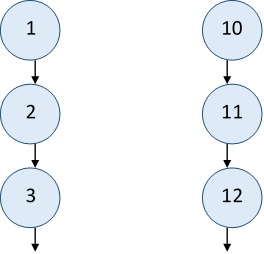
\includegraphics[angle=0,scale=0.5]{Figures/Laub/Ausgangslage.jpg}}
\captionof{figure}{Ausgangslage}
\label{imageAusgangslage}
\end{minipage}
\end{center}

\noindent In dem oberen Beispiel sind zwei Harkfolgen zu sehen, die zu verschiedenen Clustern gehören. Das Verfahren ersetzt nun den Nachfolger eines Knotens durch einen anderen, wenn die Nachfolgerbedingungen erhalten bleiben und der Zielfunktionswert dadurch geringer wird. Die Vorgänger dieses Knotens bleiben seine Vorgänger, werden also in die neue Harkfolge mitgenommen. In diesem Beispiel bekommt der Knoten 2 als neuen Nachfolger den Knoten 11 bzw. wird der Knoten 2 nun Vorgänger des Knotens 11, also $s(2)=11$ statt $s(2)=3$.

\begin{center}
\begin{minipage}{\textwidth}
\centerline{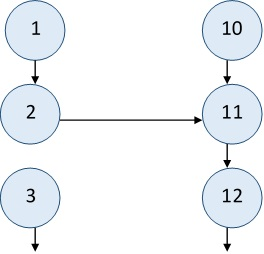
\includegraphics[angle=0,scale=0.5]{Figures/Laub/Neue_Clusterung.jpg}}
\captionof{figure}{Neue Clusterbildung}
\label{imageNeue_Clusterung}
\end{minipage}
\end{center}

\noindent Die Harkfolge ändert sich somit dahingehend, dass der Knoten 11 nun zwei Vorgänger hat, der Knoten 3 hat keine Vorgänger mehr. Die Nachbarschaftsbedingungen und die Eindeutigkeit der Zuweisungen bleiben weiterhin bestehen.\footnote{Eine algorithmische Beschreibung findet sich als Algorithmus \ref{Verbesserung durch Einfügestrategie} im Anhang \ref{Anhang_Algorithmen}.} \\
\\
Diese Art des Harkfolgentausches basiert auf dem sog. \textit{Relocate-Verfahren} von
Savelsbergh \cite{savelsbergh}. Diese Heuristik wurde entwickelt, um in der Tourenplanung entwickelte Routen zu verbessern. Hierbei wird ein Knoten aus einer Route entnommen und in eine andere Route eingefügt. Dieses Verfahren wurde von 
Van Breedam \cite{breedam} dahingehend modifiziert, dass nicht nur ein einzelner Knoten zwischen zwei Touren getauscht wird, sondern eine Kette von Knoten. 
Dieses Prinzip wird in abgewandelter Form in diesem Verbesserungsverfahren 
angewandt. Indem ein Knoten (\glqq Einfügeknoten\grqq{}) einen neuen Nachfolger in einem anderen Cluster erhält, zieht dieser Knoten seine eigenen Vorgänger mit in das neue Cluster. Insbesondere werden dabei weitere Harkquellen dem erweiterten Cluster zugefügt. Anders als beim Tourenplanungsproblem wird dieser Einfügeknoten $a$ aber nicht zwischen zwei Knoten platziert, sondern dem neuen Nachfolger \glqq vorgelagert\grqq{}.


\subsection{Lösungsverbesserung durch Clustervereinigung}
\label{subsectionClustervereinigung}

Es hat sich gezeigt, dass die Konstruktionsverfahren oft auch \glqq kleine\grqq{} Cluster erzeugen (im Extremfall sogar einelementige Cluster), bei denen die kumulierte Harklaubmenge $M^*_s(h)$ im zugehörigen Hub $h$ sehr klein ausfällt. Daher kann es -- insbesondere auch im Hinblick auf den Transportprozess -- opportun sein, benachbarte Cluster zusammenzulegen, wobei allerdings die Kapazitätsrestriktionen im Auge zu halten sind. \\
\\
Ein Prozess zur Clustervereinigung könnte folgendermaßen aussehen\footnote{Hierzu siehe Algorithmus \ref{Algo_Clustervereinigung} im Anhang \ref{Anhang_Algorithmen}.}:\\
In einem ausgewählten Cluster $C_i$ mit dem Hub $h_i$ und der kumulierten Laubharkmenge $M^*_s(h_i)$ wird jeder Knoten $a \in C_i$ daraufhin geprüft, ob dieser in $G$ zu einem Knoten $b \in V\setminus C_i$ benachbart ist. Das Cluster eines gefundenen Nachbarknotens $b$ sei $C_j$ mit dem Hub $h_j$ und der kumulierten Laubharkmenge $M^*_s(h_j)$. Falls die Vereinigung dieser beiden Cluster zulässig ist, d.h. die gemeinsame Laubharkmenge erfüllt die Kapazitätsbedingung, wird ein temporärer Harkplan entworfen, bei dem alle Knoten in $C_i$ auf Knoten $a$ als neues Hub ausgerichtet werden und die Laubharkmenge $M^*_s(h_i)$ von dort zum Knoten $b$ und weiter zum Hub $h_j$ geharkt wird. Dieser neue Harkplan wird daraufhin überprüft, ob er kostengünstiger als der bisherige Harkplan ist. Falls dem so ist, wird die entsprechende Nachfolgerfunktion $s_{neu}$, die sich insbesondere dadurch kennzeichnet, dass sie  ein Cluster weniger induziert, übernommen; andernfalls wird die Suche nach \glqq Übergangsknoten\grqq{} $a$ und $b$ fortgesetzt, bis sich kein Knotenpaar mehr finden lässt.\\
\\
Zur Auswahl von geeigneten Clustern zur Vereinigung könnte eine Schranke für die kumulierte Laubharkmenge gesetzt werden, sodass nur hinreichend kleine Cluster einem potentiellen Vereinigungsprozess zugeführt werden.








%\newpage
\begin{thebibliography}{16}

\addcontentsline{toc}{chapter}{Literaturverzeichnis}

\bibitem{clarke_wright} Clarke G, Wright JW: \textit{Scheduling vehicles from central delivery depot to a number of delivery points}. Operations Research Quarterly 12:568-581, 1964.

\bibitem{domschke_drexl} Domschke W, Drexl A: \textit{Logistik: Standorte}; 4. Auflage. Oldenbourg 2014.

\bibitem{domschke_scholl} Domschke W, Scholl A: \textit{Logistik: Rundreisen und Touren}; 5. Auflage. Oldenbourg 2010.

\bibitem{felker} Felker E: \textit{Analyse der unproduktiven Wegezeiten beim Laubharkproblem}. Bachelorarbeit im Studiengang Angewandte Mathematik der Fachhochschule Bielefeld, 2016.

\bibitem{kruse} Kruse H-J: \textit{Mathematische Modellierung des Laubharkproblems als spezielle Ausprägung von allgemeinen Entsorgungsprozessen}. In: Kruse H-J, Lask T (Hrsg.): \textit{Angewandte mathematische Modellierung und Optimierung - Ausgewählte Modelle, Methoden, Fallstudien}. Forschungsreihe des Fachbereichs Ingenieurwissenschaften und Mathematik, Band 4, Fachhochschule Bielefeld, 2016 [ISSN 2196-6192] S. 62-88.

\bibitem{kruse_et_al} Kruse H-J, Spenst N, Derdau R: \textit{Heuristische Lösungsstrategien für das Laubharkproblem}. In: Kruse H-J, Lask T (Hrsg.): \textit{Angewandte mathematische Modellierung und Optimierung - Ausgewählte Modelle, Methoden, Fallstudien}. Forschungsreihe des Fachbereichs Ingenieurwissenschaften und Mathematik, Band 4, Fachhochschule Bielefeld, 2016 [ISSN 2196-6192] S. 89-116.

\bibitem{savelsbergh} Savelsbergh MWP: \textit{The vehicle routing problem with time windows: Minimizing route duration}. Journal on Computing, 4:146-154, 1992.

\bibitem{spenst} Spenst N: \textit{Entwicklung und Implementierung von effizienten Lösungsverfahren für ein spezielles Entsorgungsproblem}. Masterarbeit im Studiengang Optimierung und Simulation der Fachhochschule Bielefeld, 2015.

\bibitem{breedam} Van Breedam A: \textit{Comparising descent heuristics and metaheuristics for the vehicle routing problem}. Computers and Operations Research, 28:289-315, 2001.

\end{thebibliography}

\appendix
\chapter*{Anhang}\label{Anhang}

\begin{tabular}{ll}
\bf Anhang \ref{Anhang_Glossar}: &\bf Glossar\\
\bf Anhang \ref{Anhang_Algorithmen}: &\bf Algorithmen\\
\bf Anhang \ref{Anhang_Beispiele}: &\bf Lösungsstrategien an Beispielen
\end{tabular}

\chapter{Glossar}\label{Anhang_Glossar}

\begin{tabular}{lp{12cm}cm{1cm}}
\textbf{Bezeichner} & \textbf{Bedeutung} & \textbf{Seite}\\
\hline
$a \in \mathbb{N}$ 
& \textbf{Feld} eines Gartens
& \pageref{Felder}\\

$G=(V,E)$
& \textbf{Graph}, durch den der Garten modellhaft beschrieben wird
& \pageref{Graph}\\

$V$
& \textbf{Knotenmenge} des Graphen $G$; entspricht den Feldern des durch $G$ modellierten Gartens
& \pageref{Knotenmenge}\\

$E$
& \textbf{Kantenmenge} des Graphen $G$; beschreibt die Nachbarschaft der Felder des durch $G$ modellierten Gartens
& \pageref{Kantenmenge}\\

$C$
& \textbf{Bewertungsmatrix} eines kantenbewerteten Graphen
& \pageref{Bewertungsmatrix}\\

$D$
& \textbf{Entfernungsmatrix} eines kantenbewerteten Graphen
& \pageref{Entfernungsmatrix}\\

$s: V \rightarrow V$ 
& \textbf{Nachfolgerfunktion}, wenn die \textit{Nachbarschaftsbedingung} (\ref{HJKmlp_equation_Nachbarschaftsbedingung}) gilt und der durch $s$ $\rightarrow$\textit{induzierte Teilgraph} $\vec{G}_s$ zyklenfrei ist
& \pageref{Nachfolgerfunktion}\\

$\vec{G}_s = \langle V,\vec{E}_s \rangle$
& durch die $\rightarrow$\textit{Nachfolgerfunktion} $s$ \textbf{induzierter Teilgraph} von $G=(V,E)$ mit $\vec{E}_s = \{\langle a,s(a)\rangle \mid a\in V \wedge a \neq s(a)\}$
& \pageref{induzierter Teilgraph}\\

$h \in V$
& \textbf{Haufenfeld} oder \textbf{Hub} $\equiv$ Senke des durch die $\rightarrow$\textit{Nachfolgerfunktion} $s$ $\rightarrow$\textit{induzierten Teilgraphen} $\vec{G}_s$, d.h. $s(h)=h$
& \pageref{Hub}\\

$Hub(s)$
& \textbf{Hubmenge} $\equiv$ Menge aller $\rightarrow$\textit{Haufenfelder} ($\rightarrow$\textit{Hubs}), welche durch die $\rightarrow$\textit{Nachfolgerfunktion} $s$ induziert werden 
& \pageref{Hubmenge}\\

$q \in V$
& \textbf{Harkquelle} $\equiv$ Quelle des durch die $\rightarrow$\textit{Nachfolgerfunktion} $s$ $\rightarrow$\textit{induzierten Teilgraphen} $\vec{G}_s$
& \pageref{Harkquelle}\\

$Q(s)$
& \textbf{Harkquellenmenge} $\equiv$ Menge aller $\rightarrow$\textit{Harkquellen}, welche durch die $\rightarrow$\textit{Nachfolgerfunktion} $s$ induziert werden 
& \pageref{Harkquellenmenge}\\

$K \in V$
& \textbf{Kompostfeld} $\equiv$ Kompoststelle des Gartens
& \pageref{Kompostfeld}\\

$M(a)$ 
& initiale \textbf{Laubmenge} in $\rightarrow$\textit{Feld} $a$; entspricht der Knotenbewertung des  $\rightarrow$\textit{Graphen} $G$
& \pageref{Laubmenge}\\

$M^*(a)$
& \textbf{aktuelle Laubmenge} in $\rightarrow$\textit{Feld} $a$; gibt die (zwischenzeitlich) kumulierte Laubmenge in Feld $a$ zum Zeitpunkt des Harkens von Feld $a$ zu einem Nachbarfeld an
& \pageref{aktuelle Laubmenge}\\

$M_k$
& \textbf{kritische Laubharkmenge}; entspricht der Laubmenge, die noch mit einem einzigen Harkzug bewegt werden kann
& \pageref{kritische Laubharkmenge}\\

$\overline{M}, \overline{M}(a)$
& \textbf{maximale Laubmenge} (von $\rightarrow$\textit{Feld} $a$); entspricht der Laubmenge, die maximal im Feld $a$ angehäuft werden kann
& \pageref{maximale Laubmenge}\\

$M^*_s:V \rightarrow \mathbb{R}_\geq$
& die durch die $\rightarrow$\textit{Nachfolgerfunktion} $s$ induzierte \textbf{Anhäufungsfunktion} gemäß Bildungsvorschrift (\ref{Definition_Anhäufungsfunktion})
& \pageref{Anhäufungsfunktion},\pageref{Anhäufungsfunktion_2} \\
\end{tabular}



\begin{tabular}{lp{11cm}cm{1cm}}
\textbf{Bezeichner} & \textbf{Bedeutung} & \textbf{Seite}\\
\hline

$\alpha_H$, $\alpha_H(a,b)$
& \textbf{Harkaufwandsfaktor} oder \textbf{Harkparameter}
& \pageref{Harkaufwandsfaktor}\\

$HA(a,b)$
& einzelner \textbf{Harkaufwand}; entspricht dem Aufwand für das Harken der aktuellen Laubmenge von Feld $a$ in ein benachbartes Feld $b$
& \pageref{Harkaufwand}f\\

$HA_{\Sigma}(s)$
&\textbf{Harkaufwandsumme}; entspricht dem Gesamtaufwand des produktiven Harkprozesses, der durch die $\rightarrow$\textit{Nachfolgerfunktion} $s$ beschrieben wird
&\pageref{Formel_Harkaufwandsumme}\\

$\alpha_W$, $\alpha_W(a,q)$
& \textbf{Wegeaufwandsfaktor} oder \textbf{Wegeparameter}
& \pageref{Wegeaufwandsfaktor}\\

$W(s)$
&\textbf{unproduktive Weglänge}; entspricht der Gesamtlänge aller unproduktiven Wege, welche durch die $\rightarrow$\textit{Nachfolgerfunktion} $s$ hervorgerufen werden
& \pageref{Wegeaufwandsfaktor}\\

$WA_{\Sigma}(s)$
&\textbf{unproduktiver Wegeaufwand}; entspricht dem Gesamtaufwand für unproduktive Wege des durch die $\rightarrow$\textit{Nachfolgerfunktion} $s$ beschriebenen Harkprozesses
& \pageref{Wegeaufwandsfaktor}f\\

$\alpha_T$
& \textbf{Transportaufwandsfaktor} oder \textbf{Transportparameter}
& \pageref{Transportaufwandsfaktor}\\

$\overline{T}$
& \textbf{maximales Ladevolumen} des Transportmittels
& \pageref{Ladevolumen}\\

$\gamma$
& \textbf{variabler Ladeaufwand} $\equiv$ variabler Aufwandsanteil für Auf- und Abladen einer Laubmenge 
& \pageref{variabler Ladeaufwand}\\

$\sigma$
& \textbf{fixer Ladeaufwand} $\equiv$ fixer Aufwandsanteil für Auf- und Abladen einer Laubmenge
& \pageref{fixer Ladeaufwand}\\

$TA(h)$
& \textbf{Transportaufwand} von $\rightarrow$\textit{Hub} $h$ zum $\rightarrow$\textit{Kompostfeld} $K$; entspricht dem Aufwand für das Transportieren der kumulierten Laubmenge von $\rightarrow$\textit{Hub} $h$ zum $\rightarrow$\textit{Kompostfeld} $K$, einschließlich der Aufwände für das Auf- und Abladen
& \pageref{Transportaufwandsfaktor}\\

$TA_{\Sigma}(s)$
& \textbf{Transportaufwandsumme}; ergibt sich als gesamter Transportaufwand aller Touren zwischen allen $\rightarrow$\textit{Hubs} bzgl. $\rightarrow$\textit{Nachfolgerfunktion} $s$ und $\rightarrow$\textit{Kompostfeld}, einschließlich aller Aufwände für das Auf- und Abladen
&\pageref{Transportaufwandsformel_5}\\

$M^{**}_s(h)$
&eine nach entsprechend vielen Pendeltouren verbleibende \textbf{Laubrestmenge} beim $\rightarrow$\textit{Hub} $h$
&\pageref{Laubrestmenge}\\

$\pi:V \leftrightarrow V$
& Permutation zur \textbf{Ausrichtung} einer $\rightarrow$\textit{Nachfolgerfunktion} $s$
& \pageref{Ausrichtung}\\

$R(a)$
&\textbf{Erreichbarkeitsmenge}; enthält alle Knoten $i \in V$, von denen aus der Knoten $a$ entlang einer Pfeilfolge im $\rightarrow$\textit{induzierten Teilgraph} $\vec{G}_s$ erreichbar ist
& \pageref{Erreichbarkeitsmenge},\pageref{Erreichbarkeitsmenge_2}\\

$C(h)$
& \textbf{Cluster}; entspricht der $\rightarrow$\textit{Erreichbarkeitsmenge} einer Senke $h$ des  $\rightarrow$\textit{induzierten Teilgraphen} $\vec{G}_s$
&\pageref{Cluster}\\

$\Lambda(G)$
& \textbf{Lösungsraum} des Laubharkproblems 
&\pageref{Lambda}\\

$K$
& \textbf{Kostenfunktion} als Zielfunktion des Laubharkproblems
&\pageref{Kostenfunktion}\\

\end{tabular}

































\chapter{Algorithmen}\label{Anhang_Algorithmen}

\begin{tabular}{lp{10cm}cm{2cm}}
\textbf{Lfd. Nr.} & \textbf{Bezeichnung} & \textbf{Seite}\\
\hline
Algorithmus \ref{Algo_Prüfung_Nachfolgerfunktion}: 
& Prüfung der Bedingungen einer Nachfolgerfunktion 
& \pageref{Algo_Prüfung_Nachfolgerfunktion}\\

Algorithmus \ref{Algo_Zulässigkeitsprüfung}: 
& Zulässigkeitsprüfung für Nachfolgerfunktion 
& \pageref{Algo_Zulässigkeitsprüfung}\\

Algorithmus \ref{Algo_Erreichbarkeitsmengenbestimmung}: 
& Bestimmung einer Erreichbarkeitsmenge 
& \pageref{Algo_Erreichbarkeitsmengenbestimmung}\\

Algorithmus \ref{Algo_Clusterbestimmung}: 
& Clusterbestimmung 
& \pageref{Algo_Clusterbestimmung}\\

Algorithmus \ref{Algo_Bestimmung_Harkaufwand}: 
& Berechnung des Harkaufwandes 
& \pageref{Algo_Bestimmung_Harkaufwand}\\

Algorithmus \ref{Algo_unproduktive_Wege}: 
& Berechnung des unproduktiven Wegeaufwandes 
& \pageref{Algo_unproduktive_Wege}\\

Algorithmus \ref{Algo_Ausrichtung_Nachfolgerfunktion}: 
& Ausrichtung einer Nachfolgerfunktion 
& \pageref{Algo_Ausrichtung_Nachfolgerfunktion}\\

Algorithmus \ref{Algo_Berechnung_von_HA_und_HW}: 
& Berechnung von Hark- und Wegeaufwand anhand einer ausgerichteten Nachfolgerfunktion 
& \pageref{Algo_Berechnung_von_HA_und_HW}\\

Algorithmus \ref{Algo_Berechnung_von_Transportaufwänden}: 
& Berechnung von Transportaufwänden 
& \pageref{Algo_Berechnung_von_Transportaufwänden}\\

Algorithmus \ref{Algo_Zickzack}: 
& Zickzack-Strategie
& \pageref{Algo_Zickzack}\\

Algorithmus \ref{Algo NW-Orientierung}: 
& Clusterbestimmung mit NW-Orientierung
& \pageref{Algo NW-Orientierung}\\

Algorithmus \ref{Algo Huborientiertes Verfahren TS}: 
& Huborientiertes Konstruktionsverfahren (TS)
& \pageref{Algo Huborientiertes Verfahren TS}\\

Algorithmus \ref{Algo Huborientiertes Verfahren BS}: 
& Huborientiertes Konstruktionsverfahren (BS)
& \pageref{Algo Huborientiertes Verfahren BS}\\

Algorithmus \ref{Algo_Hubausrichtung}: 
& Hubausrichtung
& \pageref{Algo_Hubausrichtung}\\

Algorithmus \ref{Algo_Einfacher_Nachfolgertausch}: 
& Lokales einfaches Nachfolgertauschverfahren
& \pageref{Algo_Einfacher_Nachfolgertausch}\\

Algorithmus \ref{Algo_Mehrfacher_Nachfolgertausch}: 
& Mehrfaches Nachfolgertauschverfahren
& \pageref{Algo_Mehrfacher_Nachfolgertausch}\\

Algorithmus \ref{Algo Verbesserung durch Einfügestrategie}: 
& Verbesserung durch Einfügestrategie
& \pageref{Algo Verbesserung durch Einfügestrategie}\\

Algorithmus \ref{Algo_Clustervereinigung}: 
& Verbesserung durch Clustervereinigung
& \pageref{Algo_Clustervereinigung}\\
\end{tabular}\\









\newpage
\begin{algo}[Prüfung der Bedingungen einer Nachfolgerfunktion] \label{Algo_Prüfung_Nachfolgerfunktion}
\textbf{Vorgabe:} Graph $G=[V,E]$, Abbildung $s:V \rightarrow V$.

\noindent 
\textbf{Schritt 1:} (Initialisierung)\\
\phantom \quad Setze: $H := \emptyset; N := \emptyset; Q := \emptyset$. \\
\phantom \quad Für alle $i \in V$ setze: $\delta(i):=0.$

\noindent 
\textbf{Schritt 2:} (Bestimmung der Harkquellen)\\
\phantom \quad Für alle $i \in V$ führe aus:\\
\phantom \quad \qquad Falls $i \neq s(i)$, setze: $\delta(s(i)):=\delta(s(i))+1$.\\
\phantom \quad Für alle $i \in V$ führe aus:\\
\phantom \quad \qquad Falls $\delta(i)=0$, setze: $Q := Q \cup \{i\}$\\
\phantom \quad Falls $Q=\emptyset$, terminiere! \footnote{Der durch die Abbildung $s$ beschriebene Digraph besitzt keine Quelle und ist somit nicht zyklenfrei.}

\noindent 
\textbf{Schritt 3:} (Prüfe Nachbarschaftsbedingung)\\
\phantom \quad Für alle $i \in V$ führe aus:\\
\phantom \quad \qquad Falls $[i,s(i)] \notin E$, terminiere! \footnote{Die Nachbarschaftsbedingung wird verletzt.}

\noindent 
\textbf{Schritt 4:} (Auswahl einer Harkquelle)\\
\phantom \quad Wähle $k \in Q$.\footnote{Das Auswahlkriterium ist freigestellt; es könnte beispielsweise ein Schlangen- oder Stapelspeicher zugrundegelegt werden (d.h. FIFO- oder LIFO-Prinzip).}\\
\phantom \quad Setze: $Q := Q\setminus \{k\}$.

\noindent 
\textbf{Schritt 5:} (Prüfe Zyklenfreiheit)\\
\phantom \quad Falls $s(k) \in N$, terminiere! \footnote{Der durch die Abbildung $s$ beschriebene Digraph enthält einen Zyklus.}\\
\phantom \quad Falls $s(k)=k$, führe aus:\\
\phantom \quad \qquad $H := H \cup \{k\}$.\\
\phantom \quad \qquad Falls $Q = \emptyset$, terminiere! \footnote{Die Überprüfung ist abgeschlossen, indem sämtliche Knoten des Digraphen untersucht worden sind.}\\
\phantom \quad \qquad Gehe zu Schritt 4.\\
\phantom \quad $N:=N \cup \{k\}$.\\
\phantom \quad Setze: $\delta(s(k)):=\delta(s(k))-1$.\\
\phantom \quad Falls $\delta(s(k)) \neq 0$, führe aus:\\
\phantom \quad \qquad Falls $Q=\emptyset$, terminiere! \footnote{Widerspruch zur Zyklenfreiheit.}\\
\phantom \quad \qquad Gehe zu Schritt 4.\\
\phantom \quad Setze: $k:=s(k)$ und gehe zu Schritt 5.
\end{algo}

\phantom \\
\noindent Nach Überprüfung aller Knoten enthält die Menge $H$ alle Hubs (Haufenfelder), die Menge $N$ alle Nicht-Hubs für den durch die Nachfolgerfunktion $s$ beschriebenen Harkprozess.\\


\begin{algo}[Zulässigkeitsprüfung für Nachfolgerfunktion]
\label{Algo_Zulässigkeitsprüfung}
\textbf{Vorgabe:} Graph $G=[V,E]$ mit Knotenbewertung $M:V \rightarrow \mathbb{R}_\geq$,\\ Kapazitätsfunktion $\overline{M}:V \rightarrow \mathbb{R}_\geq$, Nachfolgerfunktion $s:V \rightarrow V$, \\Quellenmenge $Q \subset V$, Eingangsvalenzen $\delta(i)$ aller Knoten $i \in V$.\footnote{Zur Bestimmung von $Q$ und der Eingangsvalenzen $\delta(i)$ vgl. Schritt 2 in Algorithmus \ref{Algo_Prüfung_Nachfolgerfunktion}.}

\noindent 
\textbf{Schritt 1:} (Vorprüfung)\\
\phantom \quad Für alle $a \in V$ führe aus:\\
\phantom \quad \qquad Falls $M(a) > \overline{M}(a)$, terminiere.\footnote{Der Initialzustand ist bereits unzulässig.}

\noindent 
\textbf{Schritt 2:} (Auswahl einer Harkquelle)\\
\phantom \quad Falls $Q = \emptyset$, terminiere.\\
\phantom \quad Wähle $k \in Q$.\\
\phantom \quad Setze: $Q := Q \setminus \{k\}, M_{kum}(k) := M(k)$.

\noindent 
\textbf{Schritt 3:} (Zulässigkeitsprüfung)\\
\phantom \quad Falls $s(k) = k$, gehe zu Schritt 2.\\
\phantom \quad Falls $M_{kum}(k) + M_{kum}(s(k)) > \overline{M}(s(k))$, terminiere.\footnote{Die Nachfolgerfunktion $s$ ist nicht zulässig bzgl. $\overline{M}$.}\\
\phantom \quad Setze: $M_{kum}(s(k)) := M_{kum}(s(k)) + M_{kum}(k) , \delta(s(k)) := \delta(s(k)) -1$.\\
\phantom \quad Falls $\delta(s(k)) \neq 0$, gehe zu Schritt 2.\\
\phantom \quad Setze: $k = s(k)$.\\
\phantom \quad Gehe zu Schritt 3.
\end{algo}

\phantom \\
\noindent Für eine zulässige Nachfolgerfunktion $s$ ist mit $M_{kum}$ die zugehörige Anhäufungsfunktion bestimmt. Das verwendete Suchprinzip entspricht dem sukzessiven Entblättern eines Baumes. Zur Bestimmung der kumulierten Laubmenge für nur einen ausgewählten Knoten $a$ bietet sich auch das umgekehrte Suchprinzip an; hierzu vgl. Algorithmus \ref{Algo_Erreichbarkeitsmengenbestimmung}. \\


%\phantom \\
\begin{algo}[Bestimmung einer Erreichbarkeitsmenge] \label{Algo_Erreichbarkeitsmengenbestimmung}
\textbf{Vorgabe}: Nachfolgerfunktion $s:V\rightarrow V$, bestimmter Knoten $a \in V$.

\noindent 
\textbf{Schritt 1:} (Initialisierung)\\
\phantom \quad Setze $K := \{a\}$, $R := \{a\}$.

\noindent 
\textbf{Schritt 2:}\\
\phantom \quad Wähle $k \in K$. \\
\phantom \quad Setze: $K := K\setminus \{k\}$. \\
\phantom \quad Für alle $i \in V\setminus R$ führe aus:\\
\phantom \quad \qquad Falls $s(i) = k$, setze: $K := K \cup \{i\}, R := R \cup \{i\}$.\\
\phantom \quad Falls $K = \emptyset$, terminiere;.\\
\phantom \quad andernfalls gehe zu Schritt 2.
\end{algo}


\phantom \\
\noindent Die Menge $R$ enthält sämtliche Knoten, von denen aus im Digraph $\vec{G}_s$ der ausgezeichnete Knoten $a$ über eine Pfeilfolge in $\vec{G}_s$ erreichbar ist; es handelt sich somit um die sog. Erreichbarkeitsmenge $R(a)$. Die Bestimmung der durch die Nachfolgerfunktion $s$ induzierten kumulierten Laubmenge im Knoten $a$ ergibt sich durch Aufsummierung $M^s(a) := \sum\limits_{i \in R(a)}M(i)$. Diese Aufsummierung ließe sich ohne Weiteres auch im Algorithmus \ref{Algo_Erreichbarkeitsmengenbestimmung} integrieren.\\

%\phantom \\
\begin{algo}[Clusterbestimmung]
\label{Algo_Clusterbestimmung}
\textbf{Vorgabe}: Nachfolgerfunktion $s$, Hubmenge $H$, Quellenmenge $Q$.\footnote{Die Mengen $H$ und $Q$ lassen sich gemäß Algorithmus \ref{Algo_Prüfung_Nachfolgerfunktion} bestimmen.}

\noindent 
\textbf{Schritt 1:} (Initialisierung)\\
\phantom \quad Für alle $h \in H$ setze: $C[h] := \{h\}$.\footnote{Alternativ könnte auch die Setzung $C[h] := \emptyset$ implementiert werden, wenn die Cluster $C[h]$ die Hubs h selbst nicht beinhalten sollen.} 

\noindent 
\textbf{Schritt 2:}\\
\phantom \quad Wähle $k \in Q$. \\
\phantom \quad Setze: $Q := Q\setminus \{k\}, T := \{k\}$.

\noindent 
\textbf{Schritt 3:}\\
\phantom \quad Falls $s(k) \in H$, führe aus:\\
\phantom \quad \qquad Setze: $C[s(k)] := C[s(k)] \cup T$.\\
\phantom \quad \qquad Falls $Q = \emptyset$, terminiere; andernfalls gehe zu Schritt 2.\\
\phantom \quad Setze: $k := s(k), T := T \cup \{k\}$.\\
\phantom \quad Gehe zu Schritt 3.
\end{algo}

\phantom \\
\noindent Die Menge C[h] enthält diejenigen Knoten (Felder), von denen gemäß Nachfolgerfunktion $s$ zum Hubfeld h geharkt wird, wobei das Hubfeld h selbst auch zum Cluster C[h] gehört.\footnote{Um diese reflexive Zuweisung auszuschließen, müsste die Setzung entsprechend geändert werden.} Diese explizite Clusterbestimmung ließe sich ohne Weiteres auch in den Algorithmus \ref{Algo_Prüfung_Nachfolgerfunktion} integrieren. \\


%\phantom \\
\begin{algo}[Berechnung des Harkaufwandes]\label{Algo_Bestimmung_Harkaufwand}
\textbf{Vorgabe}: Graph $G=[V,E]$, Knotenbewertung $M:V \rightarrow \mathbb{R}_\geq$, Kantenbewertung $\alpha_H: E \rightarrow \mathbb{R}_\geq$, zulässige Nachfolgerfunktion $s$ mit zugehöriger Anhäufungsfunktion $M^*_s$.\footnote{Zur Prüfung der Zulässigkeit von $s$ sowie Ermittlung der Anhäufungsfunktion siehe Algorithmus \ref{Algo_Zulässigkeitsprüfung}.}

\noindent 
\textbf{Schritt 1:} (Initialisierung)\\
\phantom \quad Setze: $HA_{\Sigma}(s) := 0$. 

\noindent 
\textbf{Schritt 2:} (Berechnung)\\
\phantom \quad Für alle $a \in V$ führe aus:\\
\phantom \quad \qquad Falls $a \neq s(a)$, setze: $HA_{\Sigma}(s) := HA_{\Sigma}(s) + HA(a,s(a))$.\footnote{Die Einzelaufwände $HA(a,s(a))$ ergeben sich gemäß Harkaufwandsformel (\ref{Harkaufwandsformel_1}), (\ref{Harkaufwandsformel_2}) oder (\ref{Harkaufwandsformel_3}).}
\end{algo}

\phantom \\
\noindent Der Wert $HA_{\Sigma}(s)$ gibt den reinen Harkaufwand des durch die vorgegebene Nachfolgerfunktion $s$ definierten Harkprozessen an (ohne Berücksichtigung unproduktiver Wege).\\

\begin{algo}[Berechnung des unproduktiven Wegeaufwandes]\label{Algo_unproduktive_Wege}
\textbf{Vorgabe}: Nachfolgerfunktion $s$, Entfernungsmatrix $D = (d_{ij})_{i,j \in V}$ des bewerteten Graphen $G=[V,E,c]$, Eingangsvalenzen $\delta(i)$ aller Knoten $i \in V$, Quellenmenge $Q$ sowie ein aktuelles Feld $a \in V$.\footnote{Die Eingangsvalenzen $\delta(i)$ inkl. Menge $Q$ ergeben sich gemäß Schritt 2 von Algorithmus \ref{Algo_Prüfung_Nachfolgerfunktion}.}

\noindent 
\textbf{Schritt 1:} (Initialisierung)\\
\phantom \quad Setze $u := 0$.

\noindent 
\textbf{Schritt 2:}\\
\phantom \quad Falls $Q = \emptyset$, terminiere! \\
\phantom \quad Bestimme $k \in Q$ mit $d_{ak} = min\{d_{ai} \mid i \in Q\}$.\footnote{Dieses spezielle Suchkriterium vom Greedy-Typ kann im Sinne der Optimierung des Gesamtaufwandes durch andere Suchkriterien ersetzt werden. Allgemein könnte man hier zunächst auch schreiben: Wähle $k \in Q$.} \\
\phantom \quad Setze: $Q := Q\setminus \{k\}, u := u + d_{ak}$.

\noindent 
\textbf{Schritt 3:}\\
\phantom \quad Falls $s(k)= k$, führe aus:\\
\phantom \quad \qquad Setze: $a := k$.\\
\phantom \quad \qquad Gehe zu Schritt 2.\\
\phantom \quad Setze $\delta(s(k)) := \delta(s(k))-1$.\\
\phantom \quad Falls $\delta(s(k)) = 0$, führe aus:\\
\phantom \quad \qquad Setze: $k := s(k)$.\\
\phantom \quad \qquad Gehe zu Schritt 3.\\
\phantom \quad Setze: $a := k$.\\
\phantom \quad Gehe zu Schritt 2.
\end{algo}

\phantom \\
\noindent Der Ergebniswert $u$ gibt die Gesamtlänge aller unproduktiven Wege an, wobei eine Bewertung mittels speziellem Aufwandsfaktor noch nicht berücksichtigt ist.\\

%\phantom \\
\begin{algo}[Ausrichtung einer Nachfolgerfunktion]\label{Algo_Ausrichtung_Nachfolgerfunktion}
\textbf{Vorgabe}: Kantenbewerteter Graph $G=[V,E,c]$ mit Entfernungsmatrix $D = (d_{ij})_{i,j \in V}$, Nachfolgerfunktion $s$, Quellenmenge $Q$.\footnote{Die Berechnung der Entfernungsmatrix wird mittels einem Kürzeste-Wege-Verfahren vollzogen, z.B. dem Dijkstra-Algorithmus. Zur Bestimmung der Menge $Q=Q(s)$ der Harkquellen siehe Schritt 2 in Algorithmus \ref{Algo_Prüfung_Nachfolgerfunktion}.}

\noindent 
\textbf{Schritt 1:} (Initialisierung)\\
\phantom \quad Setze: $i := 0$. \\
\phantom \quad Wähle $a \in V$ als Startknoten. 

\noindent 
\textbf{Schritt 2:}\\
\phantom \quad Falls $Q = \emptyset$, terminiere. \\
\phantom \quad Bestimme $k \in Q$ mit $d_{ak} = \min\{d_{aj} \mid j \in Q\}$.\\
\phantom \quad Setze: $i := i+1, \pi(i) := k, Q := Q\setminus \{k\}$.

\noindent 
\textbf{Schritt 3:}\\
\phantom \quad Falls $k = s(k)$, führe aus:\\
\phantom \quad \qquad Setze: $a := k$.\\
\phantom \quad \qquad Gehe zu Schritt 2.\\
\phantom \quad Falls $\delta(s(k)) \neq 0$, führe aus:\\
\phantom \quad \qquad Setze: $a := s(k)$.\\
\phantom \quad \qquad Gehe zu Schritt 2.\\
\phantom \quad Setze: $k := s(k), i := i+1, \pi(i) := k$.\\
\phantom \quad Gehe zu Schritt 3.
\end{algo}

\phantom \\
\noindent Die Permutation $\pi : V \rightarrow V$ liefert die ausgerichtete Nachfolgerfunktion $s_{\pi}$, indem die Werte $\pi(i)$ und $s(\pi(i))$ als die $i$-te Spalte in der Tabelle der ausgerichteten Nachfolgerfunktion $s_{\pi}$ zu interpretieren sind. Es ist offensichtlich, dass sich dass Auswahlkriterium für die jeweils nächste Harkquelle auch anders gestalten ließe. Zudem sollte ein Sekundärkriterium implementiert werden für den Fall, dass das Primärkriterium ("`Nächster Nachbar"') gegebenenfalls nicht eindeutig ist; hier könnte das "`Prinzip des kleinsten Knotenindex"' angewendet werden.\\


\begin{algo}[Berechnung von Hark- und Wegeaufwand anhand einer ausgerichteten Nachfolgerfunktion]
\label{Algo_Berechnung_von_HA_und_HW}
\textbf{Vorgabe}: Ausgerichtete Nachfolgerfunktion $s$, Entfernungsmatrix $D=(d_{ij})_{i,j \in V}$ des bewerteten Graphen $G=[V,E,c]$.

\noindent 
\textbf{Schritt 1:} (Initialisierung)\\
\phantom \quad Setze $\Sigma := 0$.

\noindent 
\textbf{Schritt 2:} (Berechnung)\\
\phantom \quad Für $i=1,\dots,n-1$ führe aus:\\
\phantom \quad \qquad Falls $i \neq s(i)$, setze: $\Sigma := \Sigma + HA(i,s(i))$.\footnote{Die Einzelaufwände $HA(i,s(i))$ ergeben sich gemäß Harkaufwandsformel (\ref{Harkaufwandsformel_1}), (\ref{Harkaufwandsformel_2}) oder (\ref{Harkaufwandsformel_3}).}\\
\phantom \quad \qquad Falls $s(i) \neq i+1$, setze: $\Sigma := \Sigma + \alpha_W(s(i),i+1)\cdot d_{s(i),i+1}$.\footnote{Bei konstantem Wegeaufwandsfaktor kann auch vereinfacht $\alpha_W$ geschrieben werden.}
\end{algo}

\phantom \\
\noindent Der Wert $\Sigma$ gibt die kumulierten Hark- und Wegeaufwände an, die anhand der ausgerichteten Nachfolgerfunktion $s$ als Harkprozess hervorgerufen werden. Es ist offensichtlich, dass sich ohne Weiteres auch die produktiven Harkaufwände und die unproduktiven Wegeaufwände getrennt berechnen ließen.\\


\begin{algo}[Berechnung von Transportaufwänden]
\label{Algo_Berechnung_von_Transportaufwänden}
\textbf{Vorgabe}: Entfernungsmatrix $D=(d_{ij})_{i,j \in V}$ des bewerteten Graphen $G=[V,E,c]$, Nachfolgerfunktion $s$, Hubmenge $Hub(s)$, Anhäufungsfunktion $M^*_s$, maximale Transportkapazität $\overline{T}$, Kompostfeld $K \in V$.

\noindent 
\textbf{Schritt 1:} (Initialisierung)\\
\phantom \quad Setze: $TA_\Sigma := 0$.

\noindent 
\textbf{Schritt 2:} (Berechnung der Aufwände für Pendeltouren)\\
\phantom \quad Für alle $h \in Hub(s)$ führe aus:\\
\phantom \quad \qquad Falls $M^*_s(h) < \overline{T}$, setze: $M^{**}_s(h) := M^*_s(h)$;\\
\phantom \quad \qquad andernfalls setze: $TA_\Sigma := TA_\Sigma + TA(h), M^{**}_s(h) := M^*_s(h) - \bigl\lceil \frac{M^*_s(h)}{\overline{T}}\bigr\rceil \cdot \overline{T}$.\\
\phantom \quad Falls $M^{**}_s(h) := 0$, setze: $Hub(s) := Hub(s) \setminus \{h\}$.

\noindent 
\textbf{Schritt 3:}\\
\phantom \quad Falls $Hub(s) = \emptyset$, terminiere!\\
\phantom \quad Setze: $T:=0; a:=K$.

\noindent 
\textbf{Schritt 4:} (Zurechnung der Aufwände für Sammeltouren)\\
\phantom \quad Bestimme $h \in Hub(s)$ mit $d_{ah} = \min\{d_{aj} \mid j \in Hub(s)\}$.\\
\phantom \quad Falls $T + M^{**}_s(h) \leq \overline{T}$, führe aus:\\
\phantom \quad \qquad Setze: $T:=T+M^{**}_s(h), TA_\Sigma := TA_\Sigma+\alpha_T \cdot d_{ah}, Hub(s) := Hub(s) \setminus \{h\}$.\\
\phantom \quad \qquad Falls $Hub(s) \neq \emptyset$, führe aus:\\
\phantom \quad \qquad \qquad Setze: $a := h$.\\
\phantom \quad \qquad \qquad Gehe zu Schritt 4.\\
\phantom \quad Setze: $TA_\Sigma := TA_\Sigma + \alpha_T \cdot d_{aK}$.\\
\phantom \quad Gehe zu Schritt 3.
\end{algo}

\phantom \\
\noindent Im obigen Algorithmus sind die einfachen Transportaufwandsformeln (\ref{Transportaufwandsformel_1}) und (\ref{Sammeltourformel}) implementiert. Das Ergebnis $TA_\Sigma$ gibt den danach ermittelten gesamten Transportaufwand bzgl. Nachfolgerfunktion $s$ an. \\

\newpage

\begin{algo}[Zickzack-Strategie]
\label{Algo_Zickzack}
\textbf{Vorgabe}: Knoten- und kantenbewerteter Graph $G=[V,E,c,M]$, Kapazitätsfunktion $\overline{M}:V \rightarrow \mathbb{R}_>$.

\noindent 
\textbf{Schritt 1:} (Initialisierung)\\
\phantom \quad Für alle $a \in V$ setze: $M_{kum}(a) := M(a)$.

\noindent 
\textbf{Schritt 2:} (Aufstellen einer Zickzackfolge $\varphi$)\\
\phantom \quad Für $i=1,\dots,m$ führe aus:\\
\phantom \quad \qquad Für $j=1,\dots,n$ führe aus:\\
\phantom \quad \qquad \qquad Setze: $a := (i-1) \cdot n + j$.\\
\phantom \quad \qquad \qquad Falls $i$ gerade\footnote{Die Eigenschaft einer ganzen Zahl i, gerade zu sein, lässt sich äquivalent als $i\mod 2 = 0$ angeben bzw. prüfen.}, setze: $\varphi(a) := a$;\\
\phantom \quad \qquad \qquad andernfalls setze: $\varphi(a) := i \cdot n -j +1$.

\noindent 
\textbf{Schritt 3:} (Ermittle Nachfolgerfunktion $s$ mit Zickzackfolge)\\
\phantom \quad Falls $\varphi(m \cdot n) \in V$, setze: $s(\varphi(m \cdot n)) := \varphi(m \cdot n)$\\
\phantom \quad Für alle $a=1,\dots,m \cdot n$ führe aus:\\
\phantom \quad \qquad Falls $\varphi(a) \in V$, führe aus:\\
\phantom \quad \qquad \qquad Falls $[\varphi(a),\varphi(a+1)] \notin E$, setze: $s(\varphi(a)):=\varphi(a)$;\\
\phantom \quad \qquad \qquad andernfalls führe aus:\\
\phantom \quad \qquad \qquad \qquad Setze: $s(\varphi(a)):=\varphi(a+1)$,\\ 
\phantom \quad \qquad \qquad \qquad setze: $M_{kum}(\varphi(a+1)) := M_{kum}(\varphi(a+1)) + M_{kum}(\varphi(a))$.
\end{algo}

\phantom \\
\noindent Bei der Vorgabe der Knotenmenge $V$ wird davon ausgegangen, dass die Knotenindizes $a$ den Feldnummern $(i,j)$ eines rechteckigen Gartens mit der Dimension $m \times n$ entsprechen: $a = a(i,j) = (i-1) \cdot n + j$, wobei lediglich (nicht harkbare) Ausschlussfelder weggelassen sind (also Felder $a$ mit $M(a)=-1$). Der Ergebnisvektor $s$ stellt eine zulässige Nachfolgerfunktion von $G$ dar, die entsprechend der Konstruktionsanweisung ein waagerechtes Zickzack-Harken nachahmt. Zudem ist mit $\varphi$ bereits eine Ausrichtung von $s$ gegeben, d.h. $\pi(a) = \varphi(a)$ (vgl. S. \pageref{Ausrichtung}). Möglicherweise ist es opportun, auch Ausschlussfelder in den Ergebnisvektor $s$ aufzunehmen, etwa durch die Setzung: $s(a)=0 \Leftrightarrow a \notin V$.\\
\\
Die obige einfache Zickzack-Strategie lässt sich ohne Weiteres auch auf spaltenmäßig unterteilte Teilmatrizen anwenden. Hierzu sei die Indexfolge $1,\dots,n$ wie folgt in Teilfolgen zerlegt:
$1,\dots,n_1,n_1+1,\dots,n_2,\dots,n_{k-1}+1,\dots,n_k,\dots,n_{K-1}+1,\dots,n$. Entsprechend müsste der obige Schritt 2 wie folgt verallgemeinert werden:

\noindent \textbf{Schritt 2'}:\\
\phantom \quad Für $k=1,\dots,K$ führe aus:\\
\phantom \quad \qquad Für $i=1,\dots,m$ führe aus:\\
\phantom \quad \qquad \qquad Für $j=n_{k-1}+1,\dots,n_k$ führe aus: \dots.

\begin{algo}[Clusterbestimmung mit NW-Orientierung]
\label{Algo NW-Orientierung}
\textbf{Vorgabe}: Knotenbewerteter Graph $G=[V,E,M]$, Kapazität $\overline{M}$.

\noindent 
\textbf{Schritt 1:} (Initialisierung)\\
\phantom \quad Setze: $V^{akt} := V$.\footnote{$V^{akt}$ ist als geordnete Liste anzulegen, worin die Knoten nach aufsteigenden Indizes geordnet sind. Speziell wird jeweils das erste Element entnommen.}\\
\phantom \quad Für alle $a \in V^{akt}$ setze: $s(a) := 0$.

\noindent 
\textbf{Schritt 2:}\\
\phantom \quad Falls $V^{akt} := \emptyset$, terminiere!\\
\phantom \quad Wähle $a \in V^{akt}$.\footnote{Da $V^{akt}$ ein geordnete Liste ist, wird der Knoten in $V^{akt}$ mit dem kleinsten Index gewählt, also unter den nördlichsten Feldern das westlichste.}\\
\phantom \quad Setze: $s(a) := a, V^{akt} := V^{akt} \setminus \{a\}, M^{\ast} := M(a), k := a, N := \emptyset$.\footnote{Speziell wird $N$ als Schlangenspeicher (FIFO) angelegt.}

\noindent 
\textbf{Schritt 3:}\\
\phantom \quad Für alle $b \in V^{akt}$ mit $[b,k] \in E \wedge s(b)=0$ führe aus:\\
\phantom \quad \quad Falls $M^{\ast}+M(b) \leq \overline{M}$ führe aus:\\
\phantom \quad \quad \quad Setze: $N := N \cup \{b\}$, $s(b) := k$, $M^{\ast} := M^{\ast}+M(b)$, $V^{akt} := V^{akt}\setminus \{b\}$.\\
\phantom \quad Falls $N = \emptyset$, gehe zu Schritt 2.\\
\phantom \quad Wähle $k \in N$.\\
\phantom \quad Setze: $N := N \setminus \{k\}$.\\
\phantom \quad Gehe zu Schritt 3.
\end{algo}

%\phantom \\
\noindent Die Orientierung an der nordwestlichen Ecke bei der Bestimmung aufzunehmender Knoten entspricht dem Indexkriterium (\ref{Indexkriterium}). Analog könnte auch eine andere Eckenorientierung implementiert werden. Die sich ergebende Nachfolgerfunktion $s$ liefert eine initiale Clusterbildung, an der sich eine Hubzentrierung (vgl. Abschn. \ref{section_Hubzentrierung}) und eine Hubausrichtung (vgl. Abschn. \ref{section_Hubausrichtung} bzw. Algorithmus \ref{Algo_Hubausrichtung}) in den einzelnen Clustern anschließen sollte.\\
\\
In der obigen Beschreibung könnte auf die redundante Einführung der Variablen $k$ verzichtet werden, indem durchgängig die Variable $a$ benutzt wird. Es soll hier lediglich zwischen dem originären Hub $a$ des neu zu bildenden Clusters und den anderen Clusterknoten unterschieden werden.


\newpage
\begin{algo}[Huborientiertes Konstruktionsverfahren (TS)]
\label{Algo Huborientiertes Verfahren TS}
\textbf{Vorgabe}: Knotenbewerteter Graph $G=[V,E,M]$, Kapazität $\overline{M}$.

\noindent 
\textbf{Schritt 1:} (Initialisierung)\\
\phantom \quad Setze: $V^{akt} := V$.

\noindent 
\textbf{Schritt 2:}\\
\phantom \quad Falls $V^{akt} := \emptyset$, terminiere!\\
\phantom \quad Bestimme $a \in V^{akt}$ mit $M(a) = \max\{M(b) \mid b \in V^{akt}\}$.\\
\phantom \quad Setze: $s(a) := a, V^{akt} := V^{akt} \setminus \{a\}, M^* := M(a), k := a$.

\noindent 
\textbf{Schritt 3:}\\
\phantom \quad Setze: $N := \emptyset$.\\
\phantom \quad Für alle $b \in V^{akt}$ mit $[b,k] \in E \wedge M^* + M(b) \leq \overline{M}$ setze: $N := N \cup \{b\}$.

\noindent 
\textbf{Schritt 4:}\\
\phantom \quad Falls $N = \emptyset$, führe aus:\\
\phantom \quad \qquad Falls $s(k) = k$, gehe zu Schritt 2;\\
\phantom \quad \qquad andernfalls führe aus:\\
\phantom \quad \qquad \qquad Setze: $k := s(k)$.\\
\phantom \quad \qquad \qquad Gehe zu Schritt 3.

\noindent 
\textbf{Schritt 5:}\\
\phantom \quad Bestimme $b^* \in N$ mit $M(b^*) = \min\{M(b) \mid b \in N\}$.\\
\phantom \quad Falls $M(b^*) > M(k)$, setze: $k := s(k)$;\\
\phantom \quad andernfalls führe aus:\\
\phantom \quad \qquad Falls $M^* + M(b^*) \leq \overline{M}$, führe aus:\\
\phantom \quad \qquad \qquad Setze: $s(b^*) := k, M^* := M^* + M(b^*), V^{akt} := V^{akt} \setminus \{b^*\}, k := b^*$.\\
\phantom \quad Gehe zu Schritt 3.
\end{algo}

\phantom \\
\noindent Wenn das Minimalmengen-Kriterium in Schritt 5 durch das Maximalmengen-Kriterium ersetzt werden soll, muss eine erweiterte Kapazitätsprüfung erfolgen, sodass Schritt 5 folgende Form annimmt:\\

\noindent \textbf{Schritt} $\bf{5^*:}$\\
\phantom \quad Bestimme $b^* \in N$ mit $M(b^*) = \max\{M(b) \mid b \in N\}$.\\
\phantom \quad Falls $M(b^*) > M(k)$, setze: $k := s(k)$;\\
\phantom \quad andernfalls führe aus:\\
\phantom \quad \qquad Falls $M^* + M(b^*) \leq \overline{M}$, führe aus:\\
\phantom \quad \qquad \qquad Setze: $s(b^*) := k, M^* := M^* + M(b^*), V^{akt} := V^{akt} \setminus \{b^*\}, k := b^*$;\\
\phantom \quad \qquad andernfalls führe aus:\\
\phantom \quad \qquad \qquad Setze: $N := N \setminus \{b^*\}$.\\
\phantom \quad \qquad \qquad Gehe zu Schritt 4.\\
\phantom \quad Gehe zu Schritt 3.

\phantom \\
\noindent Die Bestimmungskriterien in den Schritten 2 und 5 (bzw. 5$^*$) sollten zwecks Eindeutigkeit um das Indexkriterium als Sekundärkriterium ergänzt werden.\\
\\
Aufgrund der Übergänge zum jeweils aktuellen Knoten findet in den obigen Implementierungen des huborientierten Konstruktionsverfahrens eine Tiefensuche (TS) statt. Eine weitere Verfahrensvariante ergibt sich durch eine Breitensuche (BS):
\\


\begin{algo}[Huborientiertes Konstruktionsverfahren (BS)]
\label{Algo Huborientiertes Verfahren BS}
\textbf{Vorgabe}: Knotenbewerteter Graph $G=[V,E,M]$, Kapazität $\overline{M}$.

\noindent 
\textbf{Schritt 1:} (Initialisierung)\\
\phantom \quad Setze: $V^{akt} := V, N := \emptyset$.  [$N$ ist Stapelspeicher!]

\noindent 
\textbf{Schritt 2:}\\
\phantom \quad Falls $V^{akt} := \emptyset$, terminiere!\\
\phantom \quad Bestimme $a \in V^{akt}$ mit $M(a) = \max\{M(b) \mid b \in V^{akt}\}$.\\
\phantom \quad Setze: $s(a) := a, V^{akt} := V^{akt} \setminus \{a\}, M^* := M(a), k := a$.

\noindent 
\textbf{Schritt 3:}\\
\phantom \quad Setze: $N^{temp} := \emptyset, \mu_{max} := 0$.\\
\phantom \quad Für alle $b \in V^{akt}\setminus N$ mit $[b,k] \in E \wedge M(b) \leq M(k)$ führe aus:\\ 
\phantom \quad \qquad Setze: $N^{temp} := N^{temp} \cup \{b\}$.\\
\phantom \quad \qquad Falls $M(b) > \mu_{max}$, setze: $\mu_{max} := M(b)$.\\
\phantom \quad Setze: $\mu := \mu_{max}$.\\
\phantom \quad Solange $\mu \geq 0 \wedge N^{temp} \neq \emptyset$, führe aus:\\
\phantom \quad \qquad Bestimme $b \in N^{temp}$ mit $M(b) = \mu$.\\
\phantom \quad \qquad Falls existent, setze: $N :=N \cup \{b\}, s^{temp}(b) := k, N^{temp} := N^{temp} \setminus \{b\}$;\\
\phantom \quad \qquad andernfalls setze: $\mu := \mu - 1$.

\noindent 
\textbf{Schritt 4:}\\
\phantom \quad Falls $N = \emptyset$, gehe zu Schritt 2.\\
\phantom \quad Bestimme $b \in N$. [Beachte: $N$ ist Stapelspeicher!]\\
\phantom \quad Setze $N := N \setminus \{b\}$.\\
\phantom \quad Falls $M^* + M(b) \leq \overline{M}$, setze: $s(b) := s^{temp}(b), M^* := M^* + M(b), V^{akt} := V^{akt} \setminus \{b\}$.\\
\phantom \quad Setze: $k := b$.\\
\phantom \quad Gehe zu Schritt 3.
\end{algo}

\phantom \\
\noindent Man beachte, dass $N$ als Stapelspeicher anzulegen ist. Die Bestimmungskriterien in den Schritten 2, 3 und 4 sollten zwecks Eindeutigkeit um das Indexkriterium ergänzt werden.


\newpage
\begin{algo}[Hubausrichtung]
\label{Algo_Hubausrichtung}
\textbf{Vorgabe}: Graph $G=[V,E]$, Cluster $C \subseteq V$, Hub $h \in V$.

\noindent 
\textbf{Schritt 1:} (Initialisierung)\\
\phantom \quad Setze: $L := \{h\}, s(h) := h, M := \emptyset$.

\noindent 
\textbf{Schritt 2:} (Zuweisung)\\
\phantom \quad Wähle $a \in L$.\\
\phantom \quad Setze: $L := L\setminus \{a\}, M := M \cup \{a\}$.\\
\phantom \quad Für alle $b \in C\setminus (M \cup L)$ führe aus:\\ 
\phantom \quad \qquad Falls $[b,a] \in E$, setze: $L := L \cup \{b\}, s(b) := a$.\\
\phantom \quad Falls $L \neq \emptyset$, gehe zu Schritt 2;\\
\phantom \quad andernfalls terminiere!
\end{algo}

\phantom \\
\noindent Der Ergebnisvektor $s$ stellt eine auf das Cluster $C$ eingeschränkte Nachfolgerfunktion dar, welche komplettiert wird, wenn der Algorithmus sukzessiv auf alle Cluster $C_1,\dots,C_k$ eines Clusterings von $G$ durchgeführt wird. Die Liste $L$ muss ein Schlangenspeicher (FIFO) sein.\\
\\
Während beim obigen Algorithmus die Knotenbearbeitung vom Hub zu den Harkquellen verläuft, beginnt der dazu alternative Algorithmus bei den Harkquellen und endet beim Hub:\\
\\
\textbf{Algorithmus \ref{Algo_Hubausrichtung}$^*$} (Hubausrichtung):\\
\textbf{Vorgabe}: Graph $G=[V,E]$, Cluster $C \subseteq V$, Hub $h \in V$.\\
\textbf{Schritt 1:} (Initialisierung)\\
\phantom \quad Setze: $d_{max} := 0$.\\
\phantom \quad Für alle $a \in C$ führe aus:\\
\phantom \quad \qquad Bestimme die Entfernung $d^C_{ah}$ vom Knoten $a$ zum Hub $h$ in C.\\
\phantom \quad \qquad Falls $d^C_{ah} > d_{max}$, setze: $d_{max} := d^C_{ah}$.

\noindent 
\textbf{Schritt 2:} (Zuweisung)\\
\phantom \quad Für alle $a \in C$ mit $d^C_{ah} = d_{max}$ führe aus:\\
\phantom \quad \qquad Bestimme $b \in C$ mit $d^C_{bh} = d_{max}-1 \wedge [a,b] \in E$.\\
\phantom \quad \qquad Setze: $s(a) := b$.\\
\phantom \quad Setze: $d_{max} := d_{max}-1$.\\
\phantom \quad Falls $d_{max} > 0$, gehe zu Schritt 2;\\
\phantom \quad andernfalls terminiere!

\newpage
\begin{algo}[Lokales einfaches Nachfolgertauschverfahren]
\label{Algo_Einfacher_Nachfolgertausch}
\textbf{Vorgabe}: Knoten- und kantenbewerteter Graph $G=[V,E,M,c]$, Kapazitätsfunktion $\overline{M}$, Zielfunktion $K$, Nachfolgerfunktion $s$, ein durch $s$ induziertes Cluster $C \subseteq V$, Knoten $a \in C$.

\noindent 
\textbf{Schritt 1:} (Initialisierung)\\
\phantom \quad Berechne $K(s)$.\\
\phantom \quad Setze: $K_{akt} := K(s), k := s(a), b_{best} := s(a)$.

\noindent 
\textbf{Schritt 2:} (Bestimmung einer neuen Zuweisung)\\
\phantom \quad Für alle $b \in C\setminus\{a\}$ führe aus:\\
\phantom \quad \qquad Falls $[a,b] \in E \wedge s(a) \neq b \wedge s(b) \neq a$, führe aus:\\
\phantom \quad \qquad \qquad Setze: $s(a) := b$.\\
\phantom \quad \qquad \qquad Prüfe, ob $s$ eine Nachfolgerfunktion ist (Algorithmus \ref{Algo_Prüfung_Nachfolgerfunktion}).\footnote{Insbesondere ist hierbei auf Zyklenfreiheit zu prüfen. Diese Prüfung kann ausgelassen werden, wenn Knoten $a$ ein Hub ist.}\\
\phantom \quad \qquad \qquad Prüfe, ob $s$ zulässig ist (Algorithmus \ref{Algo_Zulässigkeitsprüfung}).\footnote{Diese Prüfung kann weggelassen werden, wenn die Kapazitätsfunktion $\overline{M}$ konstant ist.}\\
\phantom \quad \qquad \qquad Falls Prüfungsergebnis = $TRUE$, führe aus:\\
\phantom \quad \qquad \qquad  \qquad Berechne $K(s)$.\\
\phantom \quad \qquad \qquad  \qquad Falls $K(s) < K_{akt}$, setze: $K_{akt} := K(s), b_{best} := b$.\\
\phantom \quad \qquad Setze: $s(a) := k$.\\
\phantom \quad Setze: $s(a) := b_{best}$.
\end{algo}

\phantom \\
\noindent Zu einem gegebenen Knoten $a \in C$ mit ursprünglichem Nachfolger $s(a)$ wird \textit{ein} neuer Nachfolger $b$ ermittelt, wodurch der Zielfunktionswert maximal verringert wird (falls existent); es handelt sich somit um die \textit{Best-Fit-Variante}. Die \textit{First-Fit-Variante} wäre dadurch gegeben, dass der Algorithmus bereits nach der ersten Verbesserung des Zielfunktionswertes abbricht.\\
\\
Dieses Verfahren kann auf das Cluster $C$ "`globalisiert"' werden, indem das lokale Verfahren reihum auf jeden einzelnen Knoten $a \in C$ angewendet wird. Hierzu lässt sich wieder eine First-Fit- oder Best-Fit-Variante erstellen. Man mache sich allerdings klar, dass der Rechenaufwand bei einer "`doppelten"' Best-Fit-Variante bedeutend höher als bei einer "`doppelten"' First-Fit-Variante ausfällt\footnote{Darüber hinaus ließen sich auch "`gemischte"' Varianten implementieren (First-Fit/Best-Fit oder Best-Fit/First-Fit).}, um dadurch lediglich einen einzigen Wert in der Nachfolgerfunktion zu ändern.\\
\\
Das globalisierte Verfahren kann dann solange auf die jeweils neue Nachfolgerfunktion $s$ angewendet werden, bis sich mit diesem Verfahren keine Zielfunktionsverbesserung mehr erzielen lässt  oder eine Iterationsschranke erreicht ist.

\begin{algo}[Mehrfaches Nachfolgertauschverfahren]
\label{Algo_Mehrfacher_Nachfolgertausch}
\textbf{Vorgabe}: Knoten- und kantenbewerteter Graph $G=[V,E,M,c]$, Kapazitätsfunktion $\overline{M}$, Zielfunktion $K$, Nachfolgerfunktion $s$, ein durch $s$ induziertes Cluster $C \subseteq V$ mit Hub $h$.

\noindent 
\textbf{Schritt 1:} (Initialisierung)\\
\phantom \quad Berechne $K(s)$.\\
\phantom \quad Setze: $K_{akt} := K(s)$.

\noindent 
\textbf{Schritt 2:} (Bestimmung von neuen Zuweisungen)\\
\phantom \quad Für alle $a \in C\setminus \{h\}$ führe aus:\\
\phantom \quad \qquad Für alle $b \in C\setminus\{a\}$ führe aus:\\
\phantom \quad \qquad \qquad Falls $[a,b] \in E \wedge s(a) \neq b \wedge s(b) \neq a$, führe aus:\\
\phantom \quad \qquad \qquad \qquad Setze: $k := s(a), s(a) := b$.\\
\phantom \quad \qquad \qquad \qquad Falls $s$ keine (zulässige) Nachfolgerfunktion ist\footnote{Hierzu siehe Prüfmodule beim einfachen Nachfolgertausch (Algorithmus \ref{Algo_Einfacher_Nachfolgertausch}). Dabei gelten dieselben Anmerkungen.}, setze: $s(a) := k$;\\
\phantom \quad \qquad \qquad \qquad andernfalls führe aus:\\
\phantom \quad \qquad \qquad \qquad \qquad Berechne $K(s)$.\\
\phantom \quad \qquad \qquad \qquad \qquad Falls $K(s) < K_{akt}$, setze: $K_{akt} := K(s)$;\\
\phantom \quad \qquad \qquad \qquad \qquad andernfalls setze: $s(a) := k$.
\end{algo}

\phantom \\
\noindent Im Gegensatz zum einfachen Nachfolgertausch (Algorithmus \ref{Algo_Einfacher_Nachfolgertausch}) wird die Nachfolgerfunktion $s$ bei jeder Verbesserung des Zielfunktionswertes geändert, sodass sich nach dem systematischen Durchlauf über alle Knoten $a \in C\setminus \{h\}$ mehrere Zuweisungen $s(a)$ geändert haben können.\\
\\
Durch Einfügung einer Sonderbehandlung für den Fall $a=h$ bzw. $s(a)=a$ kann das obige Verfahren für einen Durchlauf über alle $a \in C$ ergänzt werden:\\
\\
Im Fall $a=s(a)$ führe aus:\\
\phantom \quad Für alle $b \in C\setminus\{a\}$ führe aus:\\
\phantom \quad \qquad Falls $[a,b] \in E$, führe aus:\\
\phantom \quad \qquad \qquad Setze: $k := s(b), s(a) := b, s(b) := b$.\\
\phantom \quad \qquad \qquad Falls $s$ nicht zulässig\footnote{Im Falle einer konstanten Kapazitätsfunktion $\overline{M}$ kann die Zulässigkeitsprüfung entfallen.}, setze: $s(a) := a, s(b) := k$;\\
\phantom \quad \qquad \qquad andernfalls führe aus:\\
\phantom \quad \qquad \qquad \qquad Berechne $K(s)$.\\
\phantom \quad \qquad \qquad \qquad Falls $K(s) < K_{akt}$, setze: $K_{akt} := K(s)$;\\
\phantom \quad \qquad \qquad \qquad andernfalls setze: $s(a) := a, s(b) := k$.


\newpage
\begin{algo}[Verbesserung durch Einfügestrategie]
\label{Algo Verbesserung durch Einfügestrategie}
\textbf{Vorgabe}: Knoten- und kantenbewerteter Graph $G=[V,E,M,c]$, Kapazitätsfunktion $\overline{M}$, Zielfunktion $K$, Nachfolgerfunktion $s$.

\noindent 
\textbf{Schritt 1:} (Initialisierung)\\
\phantom \quad Berechne $K(s)$.\\
\phantom \quad Setze: $K_{akt} := K(s)$.

\noindent 
\textbf{Schritt 2:} (Bestimmung von neuen Zuweisungen)\\
\phantom \quad Für alle $a \in V$ mit $s(a) \neq a$ führe aus:\\
\phantom \quad \qquad Für alle $b \in V$ mit $[a,b] \in E$ führe aus:\\
\phantom \quad \qquad \qquad Setze: $k := s(a)$, $s(a):= b$.\\
\phantom \quad \qquad \qquad Falls $s$ eine zulässige Nachfolgerfunktion ist, setze: $s(a) := k$;\\
\phantom \quad \qquad \qquad andernfalls führe aus:\\
\phantom \quad \qquad \qquad \qquad Berechne K(s).\\
\phantom \quad \qquad \qquad \qquad Falls $K(s) < K_{akt}$, setze: $K_{akt} := K(s)$;\\
\phantom \quad \qquad \qquad \qquad andernfalls setze: $s(a) := k$.			
\end{algo}

\phantom \\
\noindent Eine Nachfolgerfunktion $s$ mit verbessertem Zielfunktionswert induziert in der Regel neue Cluster. Da allerdings die Hubs bei der Suche nach besseren Zuweisungen ausgeschlossen werden, ändert sich nicht die Clusteranzahl. Der Durchlauf ist solange mit jeweils neuer Lösung zu wiederholen, bis sich keine Verbesserung mehr auftut oder eine Iterationsschranke erreicht ist.\\


\begin{algo}[Verbesserung durch Clustervereinigung]
\label{Algo_Clustervereinigung}
\textbf{Vorgabe}: Knoten- und kantenbewerteter Graph $G=[V,E,M,c]$, konstante Kapazitätsschranke $\overline{M}$, Zielfunktion $K$, Nachfolgerfunktion $s$ mit induzierten Clustern $C_1,\dots,C_{\ell}$ von $G$, zugehörigen Hubs $h_1,\dots,h_{\ell}$ und kumulierten Laubharkmengen $M^*_s(h_j)$ für $j=1,\dots,\ell$; zudem Schranke $M_{krit}$ für $M^*_s$.

\noindent 
\textbf{Prozedur}:\\
\phantom \quad Für $j=1,\dots,\ell$ führe aus:\\
\phantom \quad \qquad Falls $M^*_s(h_j) \leq M_{krit}$ führe aus:\\
\phantom \quad  \qquad \qquad Für alle $a \in C_j$ führe aus:\\
\phantom \quad  \qquad \qquad \qquad Für alle $b\in V\setminus C_j$ mit $[a,b] \in E$ führe aus:\\
\phantom \quad  \qquad \qquad \qquad \qquad Setze: $k := b$.\\
\phantom \quad  \qquad \qquad \qquad \qquad Solange $k \neq s(k)$, setze: $k := s(k)$.\footnote{In dieser WHILE-Schleife wird das zum Knoten $b$ gehörende Hub $h$ ermittelt.}\\
\phantom \quad  \qquad \qquad \qquad \qquad Setze: $h := k$.\\
\phantom \quad  \qquad \qquad \qquad \qquad Falls $M^*_s(h_j)+M^*_s(h) \leq M_{krit}$ führe aus:\\
\phantom \quad  \qquad \qquad \qquad \qquad \qquad Setze $s_{temp} := s$.\\
\phantom \quad  \qquad \qquad \qquad \qquad \qquad Falls $s(a) \neq a$, richte für $s_{temp}$ alle $k \in C_j$ auf $a$ aus.\footnote{Hierzu vgl. Algorithmus \ref{Algo_Ausrichtung_Nachfolgerfunktion}.}\\
\phantom \quad  \qquad \qquad \qquad \qquad \qquad Setze $s_{temp}(a) := b$.\\
\phantom \quad  \qquad \qquad \qquad \qquad \qquad Falls $K(s_{temp}) < K(s)$, führe aus:\\
\phantom \quad  \qquad \qquad \qquad \qquad \qquad \qquad Setze: $s := s_{neu}$;\\
\phantom \quad  \qquad \qquad \qquad \qquad \qquad \qquad Terminiere!
\end{algo}

\phantom \\
\noindent Die Schranke $M_{krit}$ legt fest, ab wann ein Cluster \glqq kritisch\grqq{} ist, d.h. \glqq klein genug\grqq{}, um für einen \glqq Einschmelzungsprozess\grqq{} zugelassen zu werden. Für hinreichend großes $M_{krit}$ können auch alle Cluster zur Auswahl gestellt werden. \\
\\
Die obige Prozedurbeschreibung gilt nur für den Fall einer konstanten Kapazitätsfunktion $\overline{M}$. Eine Verallgemeinerung auf beliebige Kapazitätsfunktionen ist sehr viel aufwändiger auszuformulieren (und rechenintensiver). Darüber hinaus ist die obige Prozedur eine First-Fit-Variante, die bei der ersten Verbesserung abbricht (oder ohne Verbesserungsergebnis endet). Eine rechenintensivere Best-Fit-Variante könnte sowohl die Suche nach einem \glqq besten ersten\grqq{} Übergangsknoten $a$ als auch nach einem \glqq besten zweiten\grqq{} Übergangsknoten $b$ beinhalten. Die Prozedur ist solange zu wiederholen, bis sich keine Verbesserung mehr erzielen lässt oder eine Iterationsschranke erreicht ist.









\chapter{Lösungsstrategien am Beispiel}\label{Anhang_Beispiele}

Auf das folgende Beispiel für einen Garten in Matrixdarstellung (vgl. Abb. \ref{Beispiel_Gartenmatrix}) bzw. in Graphendarstellung (vgl. Abb. \ref{Beispiel_Gartengraph}) sollen im Folgenden einige der in Kap. \ref{chapterLösungsstrategien} behandelten Harkstrategien angewendet werden.

\begin{center}
\begin{minipage}{\textwidth}
\renewcommand{\arraystretch}{1.5}
\begin{table}[H]
\centering 
\begin{scriptsize}
\begin{tabular}{|>{}c|>{}c|>{}c|>{}c|>{}c|>{}c|>{}c|>{}c|>{}c|>{}c|>{}c|>{}c|>{}c|}
\hline
3&2&5&1&1&4&2&3&4&8&3&2&1 \\
\hline
2&2&4&\cellcolor{gray!50!white} &1&3&4&2&1&0&1&1&3 \\
\hline
1&1&2&2&\cellcolor{gray!50!white} &\cellcolor{gray!50!white} &1&3&2&1&2&3&2 \\
\hline
3&2&1&3&2&2&2&1&1&2&2&2&2 \\
\hline
4&5&3&4&3&3&1&1&0&1&1&2&2 \\
\hline
\cellcolor{gray!50!white}\bf{K}&3&3&1&2&\cellcolor{gray!50!white} &\cellcolor{gray!50!white} &0&0&2&2&4&3 \\
\hline
\end{tabular}
\captionof{figure}{Beispiel für einen Garten in Matrixdarstellung}
\label{Beispiel_Gartenmatrix}
\end{scriptsize} 
\end{table}
\renewcommand{\arraystretch}{1}
\end{minipage}
\end{center}

\begin{center}
\begin{minipage}{\textwidth}
\centerline{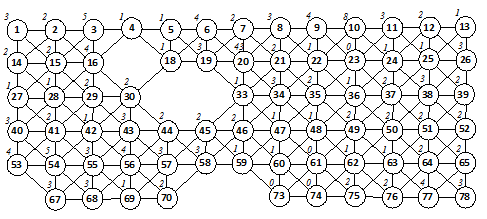
\includegraphics[angle=0,scale=1.25]{Figures/Laub/Gartengraph_Beispiel.png}}
\captionof{figure}{Beispiel für einen Garten in Graphendarstellung}
\label{Beispiel_Gartengraph}
\end{minipage}
\end{center}

\phantom \\
\noindent Es werde der Einfachheit halber angenommen, dass sämtliche Kanten mit 1 bewertet sind und die dementsprechend ermittelten Entfernungen zwischen den Knoten in der zugehörigen Matrix $D=(d_{ij})$ hinterlegt sind ($i=1,\dots,6; j=1,\dots,13$). Zudem wird das südwestliche Feld als Kompostfeld festgelegt: $K=66 \equiv (6,1)$. Die Entfernung $d_{a,K}$ von den Knoten $a$ zum Kompostfeld seien ebenfalls hinterlegt; dazu werde gesetzt: $d_{53,K}=d_{54,K}=d_{67,K}=1$. Als Anfangsfeld für den Harkprozess wird der Knoten 1 bestimmt. Zudem wird von einer konstanten Kapazitätsfunktion $\overline{M}$ ausgegangen und $\overline{M}(a)=20$ für alle $a \in V$ festgelegt. Für die Transportkapazität gelte: $\overline{T} \geq 20$; somit wird zu jedem Hub nur \textit{eine} Pendeltour benötigt.\footnote{Einsparungsmöglichkeiten durch Sammeltouren werden in \ref{Beispiel_Erläuterungen} diskutiert.}\\
\\
Jede Ergebnisdarstellung besteht aus der jeweiligen Nachfolgerfunktion $s$ in ausgerichteter Form und der Visualisierung des Harkprozesses, wobei die Pfeile die Harkrichtungen angeben, die entstandenen Cluster farbig hervorgehoben sind und in den Hubfeldern die kumulierten Laubharkmengen angegeben sind.

\section{Zickzack-Strategien am Beispiel}\label{sec_Zickzack}
%\noindent \textbf{\underline{Einfache Zickzack-Strategie am Beispiel}}\label{Zickzack_einfach}

\subsection{Einfache Zickzack-Strategie}\label{Zickzack_einfach}
\noindent Die \textit{einfache Zickzack-Strategie} liefert den folgenden Harkplan (Abb. \ref{Beispiel_Gartenmatrix_Zickzack}) mit zulässiger Nachfolgerfunktion $s$: 

\begin{center}
\begin{minipage}{\textwidth}
\renewcommand{\arraystretch}{1.2}
%\begin{table}[H]
%\caption{Ausgerichtete Nachfolgerfunktion zur einfachen Zickzack-Strategie am Beispiel}
%\centering 
\begin{scriptsize}
\begin{tabular}{|c|*{24}{|p{.15cm}}|}
\hline
$a$&1&2&3&4&5&6&\cellcolor{gray!25!white}7&8&9&10&11&\cellcolor{gray!25!white}12&13&26&25&24&23&22&21&20&19&\cellcolor{gray!25!white}18&16&15 \\
\hline
$s(a)$&2&3&4&5&6&7&\cellcolor{gray!25!white}7&9&10&11&12&\cellcolor{gray!25!white}12&26&25&24&23&22&21&20&19&18&\cellcolor{gray!25!white}18&15&14\\
\hline \hline
$a$&14&27&28&29&\cellcolor{gray!25!white}30&33&34&35&36&37&38&39&52&51&\cellcolor{gray!25!white}50&49&48&47&46&45&44&43&42&41\\
\hline
$s(a)$&27&28&29&30&\cellcolor{gray!25!white}30&34&35&36&37&38&39&52&51&50&\cellcolor{gray!25!white}50&48&47&46&45&44&43&42&41&40\\
\hline \hline
$a$&\cellcolor{gray!25!white}40&53&54&55&56&\cellcolor{gray!25!white}57&58&59&60&61&62&63&64&65&78&77&\cellcolor{gray!25!white}76&75&74&\cellcolor{gray!25!white}73&70&69&68&\cellcolor{gray!25!white}67\\
\hline
$s(a)$&\cellcolor{gray!25!white}40&54&55&56&57&\cellcolor{gray!25!white}57&59&60&61&62&63&64&65&78&77&76&\cellcolor{gray!25!white}76&74&73&\cellcolor{gray!25!white}73&69&68&67&\cellcolor{gray!25!white}67\\
\hline
\end{tabular}
\label{Beispiel_HF_Zickzack_einfach}
\end{scriptsize} 
%\end{table}
\renewcommand{\arraystretch}{1}
%\end{minipage}
%\end{center}

%\begin{center}
%\begin{minipage}{\textwidth}
\renewcommand{\arraystretch}{1.4}
\begin{table}[H]
\centering 
\begin{scriptsize}
\begin{tabular}{|>{}c|>{}c|>{}c|>{}c|>{}c|>{}c|>{}c|>{}c|>{}c|>{}c|>{}c|>{}c|>{}c|}
\hline
\cellcolor{red!15!white}$\rightarrow$&\cellcolor{red!15!white}$\rightarrow$&\cellcolor{red!15!white}$\rightarrow$&\cellcolor{red!15!white}$\rightarrow$&\cellcolor{red!15!white}$\rightarrow$&\cellcolor{red!15!white}$\rightarrow$&\cellcolor{red!15!white}\bf{18}&\cellcolor{green!15!white}
$\rightarrow$&\cellcolor{green!15!white}$\rightarrow$&\cellcolor{green!15!white}$\rightarrow$&\cellcolor{green!15!white}$\rightarrow$&\cellcolor{green!15!white}\bf{20}&\cellcolor{yellow!15!white}$\downarrow$\\
\hline
\cellcolor{green!15!white}$\downarrow$&\cellcolor{green!15!white}$\leftarrow$&\cellcolor{green!15!white}$\leftarrow$&\cellcolor{gray!50!white} &\cellcolor{yellow!15!white}\bf{17}&
\cellcolor{yellow!15!white}$\leftarrow$&\cellcolor{yellow!15!white}$\leftarrow$&\cellcolor{yellow!15!white}$\leftarrow$&\cellcolor{yellow!15!white}$\leftarrow$&\cellcolor{yellow!15!white}$\leftarrow$&\cellcolor{yellow!15!white}$\leftarrow$&\cellcolor{yellow!15!white}$\leftarrow$&\cellcolor{yellow!15!white}$\leftarrow$ \\
\hline
\cellcolor{green!15!white}$\rightarrow$&\cellcolor{green!15!white}$\rightarrow$&\cellcolor{green!15!white}$\rightarrow$&\cellcolor{green!15!white}\bf{14}&\cellcolor{gray!50!white} &\cellcolor{gray!50!white} &\cellcolor{blue!15!white}$\rightarrow$&\cellcolor{blue!15!white}$\rightarrow$&\cellcolor{blue!15!white}$\rightarrow$&\cellcolor{blue!15!white}$\rightarrow$&\cellcolor{blue!15!white}$\rightarrow$&\cellcolor{blue!15!white}$\rightarrow$&\cellcolor{blue!15!white}$\downarrow$ \\
\hline
\cellcolor{red!15!white}\bf{19}&\cellcolor{red!15!white}$\leftarrow$&\cellcolor{red!15!white}$\leftarrow$&\cellcolor{red!15!white}$\leftarrow$&\cellcolor{red!15!white}$\leftarrow$&\cellcolor{red!15!white}$\leftarrow$&\cellcolor{red!15!white}$\leftarrow$&\cellcolor{red!15!white}$\leftarrow$
&\cellcolor{red!15!white}$\leftarrow$&\cellcolor{red!15!white}$\leftarrow$&\cellcolor{blue!15!white}\bf{20}&\cellcolor{blue!15!white}$\leftarrow$&\cellcolor{blue!15!white}$\leftarrow$ \\
\hline
\cellcolor{yellow!15!white}$\rightarrow$&\cellcolor{yellow!15!white}$\rightarrow$&\cellcolor{yellow!15!white}$\rightarrow$&\cellcolor{yellow!15!white}$\rightarrow$&\cellcolor{yellow!15!white}\bf{19}&\cellcolor{green!15!white}$\rightarrow$&\cellcolor{green!15!white}$\rightarrow$
&\cellcolor{green!15!white}$\rightarrow$&\cellcolor{green!15!white}$\rightarrow$&\cellcolor{green!15!white}$\rightarrow$&\cellcolor{green!15!white}$\rightarrow$&\cellcolor{green!15!white}$\rightarrow$&\cellcolor{green!15!white}$\downarrow$\\
\hline
\cellcolor{gray!50!white} &\cellcolor{blue!15!white}\bf{9}&\cellcolor{blue!15!white}$\leftarrow$&\cellcolor{blue!15!white}$\leftarrow$&\cellcolor{blue!15!white}$\leftarrow$&\cellcolor{gray!50!white} &\cellcolor{gray!50!white} &\cellcolor{yellow!15!white}\bf{2}&\cellcolor{yellow!15!white}$\leftarrow$&\cellcolor{yellow!15!white}$\leftarrow$&\cellcolor{green!15!white}\bf{20}&\cellcolor{green!15!white}$\leftarrow$&\cellcolor{green!15!white}$\leftarrow$ \\
\hline
\end{tabular}
\captionof{figure}{Harkplan durch einfache Zickzack-Strategie am Beispiel}
\label{Beispiel_Gartenmatrix_Zickzack}
\end{scriptsize} 
\end{table}
\renewcommand{\arraystretch}{1}
\end{minipage}
\end{center}

\phantom \\
\noindent Die gesamte Laubmenge des Gartens in Höhe von 158 [ME] werden dabei auf 10 Hubs zusammengeharkt. Dabei entsteht gemäß (\ref{Harkaufwandsformel_1}) ein produktiver Harkaufwand von $HA_{\Sigma}(s)=517$ [ZE] bei Parametersetzung $\alpha_H = 1$ [ZE/ME].\footnote{Diese Standardsetzung für $\alpha_H$ erfolgt insofern o.B.d.A., da lediglich das Verhältnis zu den beiden anderen Parametern $\alpha_W$ und $\alpha_T$ das Gütemaß für eine Harkstrategie entscheidend beeinflusst.} Gemäß (\ref{Wegeaufwandsformel_1}) ergibt sich als Summe der unproduktiven Wege zu $W(s)=14$ [LE], die durch Gewichtung mit dem Wegeparameter $\alpha_W$ gemäß (\ref{Wegeaufwandsformel_2}) einen unproduktiven Wegeaufwand $WA_{\Sigma}(s) = 14 \cdot \alpha_W$ [ZE] ergibt.\footnote{Hierbei ist zu beachten, dass die Übergänge von einem erreichten Hub zur nächsten Harkquelle hierbei in Zickzack-Richtung erfolgt. Bei Beachtung des "`Nächster Nachfolger"'-Prinzips ergäben sich 18 [LE].} Für die Bestimmung des Transportaufwandes sind der Einfachheit halber ausschließlich Pendeltouren zwischen den Hubs und dem Kompostfeld zugelassen, deren Einzelaufwände gemäß (\ref{Transportaufwandsformel_1}) sich zum Gesamttransportaufwand $TA_{\Sigma} = 116\cdot \alpha_T$ [ZE] aufsummieren (vgl. (\ref{Transportaufwandsformel_5})). Demnach ergibt sich aus der einfachen Zickzack-Strategie ein Gesamtaufwand von $K(s) = 517 + 14 \cdot \alpha_W + 116\cdot \alpha_T$ [ZE]. \\
\\
Durch Anwendung von \textit{Hubzentrierung}\footnote{Hierbei wird primär das \textit{Maximalmengen-Kriterium} (\ref{Maximalmengenkriterium}), sekundär das \textit{Median-Kriterium} (\ref{Mediankriterium}) und tertiär das \textit{Indexkriterium} (\ref{Indexkriterium}) angewendet; vgl. Abschn. \ref{section_Hubzentrierung}.} und \textit{Hubausrichtung} ergibt sich der folgende Harkprozess (Abb. \ref{Beispiel_Gartenmatrix_Zickzack_mit_Hubausrichtung}) mit zugehöriger Nachfolgerfuktion $s$, wobei sich der zugehörige Gesamtaufwand auf $K(s) = 254 + 47 \cdot \alpha_W + 114 \cdot \alpha_T$ [ZE] deutlich verringert, zumal $\alpha_W \leq 1$ angenommen werden kann.


\begin{center}
\begin{minipage}{\textwidth}
\renewcommand{\arraystretch}{1.2}
%\begin{table}[H]
%\caption{Ausgerichtete Nachfolgerfunktion nach Hubausrichtung am Beispiel}
%\centering 
\begin{scriptsize}
\begin{tabular}{|c|*{24}{|p{.15cm}}|}
\hline
$a$&1&2&14&27&15&28&29&30&\cellcolor{gray!25!white}16&18&19&7&6&5&4&\cellcolor{gray!25!white}3&40&41&42&57&56&55&53&\cellcolor{gray!25!white}54 \\
\hline
$s(a)$&2&3&15&15&16&16&16&16&\cellcolor{gray!25!white}16&19&20&6&5&4&3&\cellcolor{gray!25!white}3&41&42&43&56&55&54&54&\cellcolor{gray!25!white}54\\
\hline \hline
$a$&67&70&69&\cellcolor{gray!25!white}68&58&59&60&61&62&63&64&65&76&78&\cellcolor{gray!25!white}77&49&48&47&46&45&44&\cellcolor{gray!25!white}43&33&34\\
\hline
$s(a)$&68&69&68&\cellcolor{gray!25!white}68&59&60&61&62&63&77&77&77&77&77&\cellcolor{gray!25!white}77&48&47&46&45&44&43&\cellcolor{gray!25!white}43&34&35\\
\hline \hline
$a$&35&36&37&26&11&8&9&\cellcolor{gray!25!white}10&12&13&25&24&23&22&21&\cellcolor{gray!25!white}20&50&39&51&52&\cellcolor{gray!25!white}38&73&74&\cellcolor{gray!25!white}75\\
\hline
$s(a)$&36&37&38&25&10&9&10&\cellcolor{gray!25!white}10&24&25&24&23&22&21&20&\cellcolor{gray!25!white}20&38&38&38&38&\cellcolor{gray!25!white}38&74&75&\cellcolor{gray!25!white}75\\
\hline
\end{tabular}
\label{Beispiel_HF_Zickzack_mit_Hubausrichtung}
\end{scriptsize} 
%\end{table}
\renewcommand{\arraystretch}{1}
%\end{minipage}
%\end{center}

%\begin{center}
%\begin{minipage}{\textwidth}
\renewcommand{\arraystretch}{1.4}
\begin{table}[H]
\centering 
\begin{scriptsize}
\begin{tabular}{|>{}c|>{}c|>{}c|>{}c|>{}c|>{}c|>{}c|>{}c|>{}c|>{}c|>{}c|>{}c|>{}c|}
\hline
\cellcolor{red!15!white}$\rightarrow$&\cellcolor{red!15!white}$\rightarrow$&\cellcolor{red!15!white}\bf{18}&\cellcolor{red!15!white}$\leftarrow$&\cellcolor{red!15!white}$\leftarrow$&\cellcolor{red!15!white}$\leftarrow$&\cellcolor{red!15!white}$\leftarrow$&
\cellcolor{green!15!white}$\rightarrow$&\cellcolor{green!15!white}$\rightarrow$&\cellcolor{green!15!white}$\rightarrow$&\cellcolor{green!15!white}\bf{20}&\cellcolor{green!15!white}$\leftarrow$&\cellcolor{yellow!15!white}$\swarrow$\\
\hline
\cellcolor{green!15!white}$\rightarrow$&\cellcolor{green!15!white}$\rightarrow$&\cellcolor{green!15!white}\bf{14}&\cellcolor{gray!50!white} &\cellcolor{yellow!15!white}$\rightarrow$&\cellcolor{yellow!15!white}$\rightarrow$& \cellcolor{yellow!15!white}\bf{17}&\cellcolor{yellow!15!white}$\leftarrow$&\cellcolor{yellow!15!white}$\leftarrow$&\cellcolor{yellow!15!white}$\leftarrow$&\cellcolor{yellow!15!white}$\leftarrow$&\cellcolor{yellow!15!white}$\leftarrow$&\cellcolor{yellow!15!white}$\leftarrow$ \\
\hline
\cellcolor{green!15!white}$\nearrow$&\cellcolor{green!15!white}$\nearrow$&\cellcolor{green!15!white}$\uparrow$&\cellcolor{green!15!white}$\nwarrow$&\cellcolor{gray!50!white} &\cellcolor{gray!50!white} &\cellcolor{blue!15!white}$\rightarrow$&\cellcolor{blue!15!white}$\rightarrow$&\cellcolor{blue!15!white}$\rightarrow$&\cellcolor{blue!15!white}$\rightarrow$&\cellcolor{blue!15!white}$\rightarrow$&\cellcolor{blue!15!white}\bf{20}&\cellcolor{blue!15!white}$\leftarrow$ \\
\hline
\cellcolor{red!15!white}$\rightarrow$&\cellcolor{red!15!white}$\rightarrow$&\cellcolor{red!15!white}$\rightarrow$&\cellcolor{red!15!white}\bf{19}&\cellcolor{red!15!white}$\leftarrow$&\cellcolor{red!15!white}$\leftarrow$&\cellcolor{red!15!white}$\leftarrow$&\cellcolor{red!15!white}$\leftarrow$
&\cellcolor{red!15!white}$\leftarrow$&\cellcolor{red!15!white}$\leftarrow$&\cellcolor{blue!15!white}$\nearrow$&\cellcolor{blue!15!white}$\uparrow$&\cellcolor{blue!15!white}$\nwarrow$ \\
\hline
\cellcolor{yellow!15!white}$\rightarrow$&\cellcolor{yellow!15!white}\bf{19}&\cellcolor{yellow!15!white}$\leftarrow$&\cellcolor{yellow!15!white}$\leftarrow$&\cellcolor{yellow!15!white}$\leftarrow$&\cellcolor{green!15!white}$\rightarrow$&\cellcolor{green!15!white}$\rightarrow$
&\cellcolor{green!15!white}$\rightarrow$&\cellcolor{green!15!white}$\rightarrow$&\cellcolor{green!15!white}$\rightarrow$&\cellcolor{green!15!white}$\searrow$&\cellcolor{green!15!white}$\downarrow$&\cellcolor{green!15!white}$\swarrow$\\
\hline
\cellcolor{gray!50!white} &\cellcolor{blue!15!white}$\rightarrow$&\cellcolor{blue!15!white}\bf{9}&\cellcolor{blue!15!white}$\leftarrow$&\cellcolor{blue!15!white}$\leftarrow$&\cellcolor{gray!50!white} &\cellcolor{gray!50!white} &\cellcolor{yellow!15!white}$\rightarrow$&\cellcolor{yellow!15!white}$\rightarrow$&\cellcolor{yellow!15!white}\bf{2}&\cellcolor{green!15!white}$\rightarrow$&\cellcolor{green!15!white}\bf{20}&\cellcolor{green!15!white}$\leftarrow$ \\
\hline
\end{tabular}
\captionof{figure}{Harkplan durch einfache Zickzack-Strategie nach Hubausrichtung am Beispiel}
\label{Beispiel_Gartenmatrix_Zickzack_mit_Hubausrichtung}
\end{scriptsize} 
\end{table}
\renewcommand{\arraystretch}{1}
\end{minipage}
\end{center}

%\phantom \\
\subsection{Unterteilte Zickzack-Strategie}\label{Zickzack_unterteilt}
%\noindent \textbf{\underline{Unterteilte Zickzack-Strategie am Beispiel}} \label{Zickzack_unterteilt}

\noindent Die obige Gartenmatrix wird nun in drei Teilmatrizen unterteilt: $n_1 = 4, n_2 = 10$.
Die Anwendung der \textit{unterteilten Zickzack-Strategie} führt zu folgendem Harkprozess:

\begin{center}
\begin{minipage}{\textwidth}
\renewcommand{\arraystretch}{1.2}
%\begin{table}[H]
%\caption{Ausgerichtete Nachfolgerfunktion für unterteilte Zickzack-Strategie am Beispiel}
%\centering 
\begin{scriptsize}
\begin{tabular}{|c|*{24}{|p{.15cm}}|}
\hline
$a$&1&2&3&\cellcolor{gray!25!white}4&16&15&14&27&28&29&30&43&42&\cellcolor{gray!25!white}41&40&53&54&55&\cellcolor{gray!25!white}56&69&68&\cellcolor{gray!25!white}67&5&6 \\
\hline
$s(a)$&2&3&4&\cellcolor{gray!25!white}4&15&14&27&28&29&30&43&42&41&\cellcolor{gray!25!white}41&53&54&55&56&\cellcolor{gray!25!white}56&68&67&\cellcolor{gray!25!white}67&6&7\\
\hline \hline
$a$&7&8&9&22&\cellcolor{gray!25!white}21&20&19&\cellcolor{gray!25!white}18&33&34&35&48&47&46&45&44&57&\cellcolor{gray!25!white}58&59&60&61&74&\cellcolor{gray!25!white}73&10\\
\hline
$s(a)$&8&9&22&21&\cellcolor{gray!25!white}21&19&18&\cellcolor{gray!25!white}18&34&35&48&47&46&45&44&57&58&\cellcolor{gray!25!white}58&60&61&74&73&\cellcolor{gray!25!white}73&11\\
\hline \hline
$a$&11&12&13&26&25&24&23&\cellcolor{gray!25!white}36&37&38&39&52&51&50&49&62&63&\cellcolor{gray!25!white}64&65&78&77&76&\cellcolor{gray!25!white}75&\cellcolor{gray!25!white}70\\
\hline
$s(a)$&12&13&26&25&24&23&36&\cellcolor{gray!25!white}36&38&39&52&51&50&49&62&63&64&\cellcolor{gray!25!white}64&78&77&76&75&\cellcolor{gray!25!white}75&\cellcolor{gray!25!white}70\\
\hline
\end{tabular}
\label{Beispiel_HF_Zickzack_unterteilt}
\end{scriptsize} 
%\end{table}
\renewcommand{\arraystretch}{1}
%\end{minipage}
%\end{center}

%\begin{center}
%\begin{minipage}{\textwidth}
\renewcommand{\arraystretch}{1.4}
\begin{table}[H]
\centering 
\begin{scriptsize}
\begin{tabular}{|>{}c|>{}c|>{}c|>{}c||>{}c|>{}c|>{}c|>{}c|>{}c||>{}c|>{}c|>{}c|>{}c|}
\hline
\cellcolor{red!15!white}$\rightarrow$&\cellcolor{red!15!white}$\rightarrow$&\cellcolor{red!15!white}$\rightarrow$\cellcolor{red!15!white}&\cellcolor{red!15!white}\bf{11}&
\cellcolor{green!15!white}$\rightarrow$&\cellcolor{green!15!white}$\rightarrow$&\cellcolor{green!15!white}$\rightarrow$&\cellcolor{green!15!white}$\rightarrow$&\cellcolor{green!15!white}$\downarrow$&
\cellcolor{red!15!white}$\rightarrow$&\cellcolor{red!15!white}$\rightarrow$&\cellcolor{red!15!white}$\rightarrow$&\cellcolor{red!15!white}$\downarrow$\\
\hline
\cellcolor{green!15!white}$\downarrow$&\cellcolor{green!15!white}$\leftarrow$&\cellcolor{green!15!white}$\leftarrow$&\cellcolor{gray!50!white} &
\cellcolor{yellow!15!white}\bf{8}&\cellcolor{yellow!15!white}$\leftarrow$&\cellcolor{yellow!15!white}$\leftarrow$&\cellcolor{green!15!white}\bf{17}&\cellcolor{green!15!white}$\leftarrow$&
\cellcolor{red!15!white}$\downarrow$&\cellcolor{red!15!white}$\leftarrow$&\cellcolor{red!15!white}$\leftarrow$&\cellcolor{red!15!white}$\leftarrow$ \\
\hline
\cellcolor{green!15!white}$\rightarrow$&\cellcolor{green!15!white}$\rightarrow$&\cellcolor{green!15!white}$\rightarrow$&\cellcolor{green!15!white}$\downarrow$&
\cellcolor{gray!50!white} &\cellcolor{gray!50!white} &\cellcolor{blue!15!white}$\rightarrow$ &\cellcolor{blue!15!white}$\rightarrow$ &\cellcolor{blue!15!white}$\downarrow$ &\cellcolor{red!15!white}\bf{20}&\cellcolor{green!15!white}$\rightarrow$ &\cellcolor{green!15!white}$\rightarrow$ &\cellcolor{green!15!white}$\downarrow$ \\
\hline
\cellcolor{red!15!white}$\downarrow$&\cellcolor{green!15!white}\bf{20}&\cellcolor{green!15!white}$\leftarrow$&\cellcolor{green!15!white}$\leftarrow$&
\cellcolor{blue!15!white}$\downarrow$&\cellcolor{blue!15!white}$\leftarrow$&\cellcolor{blue!15!white}$\leftarrow$&\cellcolor{blue!15!white}$\leftarrow$&\cellcolor{blue!15!white}$\leftarrow$ 
&\cellcolor{green!15!white}$\downarrow$ &\cellcolor{green!15!white}$\leftarrow$&\cellcolor{green!15!white}$\leftarrow$ &\cellcolor{green!15!white}$\leftarrow$ \\
\hline
\cellcolor{red!15!white}$\rightarrow$&\cellcolor{red!15!white}$\rightarrow$&\cellcolor{red!15!white}$\rightarrow$&\cellcolor{red!15!white}\bf{19}&
\cellcolor{blue!15!white}$\rightarrow$&\cellcolor{blue!15!white}\bf{20}&\cellcolor{red!15!white}$\rightarrow$&\cellcolor{red!15!white}$\rightarrow$&\cellcolor{red!15!white}$\downarrow$ &\cellcolor{green!15!white}$\rightarrow$&\cellcolor{green!15!white}$\rightarrow$&\cellcolor{green!15!white}\bf{19}&\cellcolor{yellow!15!white}$\downarrow$\\
\hline
\cellcolor{gray!50!white} &\cellcolor{yellow!15!white}\bf{7}&\cellcolor{yellow!15!white}$\leftarrow$&\cellcolor{yellow!15!white}$\leftarrow$&
\cellcolor{green!15!white}\bf{2}&\cellcolor{gray!50!white} &\cellcolor{gray!50!white} &\cellcolor{red!15!white}\bf{2}&\cellcolor{red!15!white}$\leftarrow$& \cellcolor{yellow!15!white}\bf{13}&\cellcolor{yellow!15!white}$\leftarrow$&\cellcolor{yellow!15!white}$\leftarrow$&\cellcolor{yellow!15!white}$\leftarrow$ \\
\hline
\end{tabular}
\captionof{figure}{Harkplan durch unterteilte Zickzack-Strategie am Beispiel}
\label{Beispiel_Gartenmatrix_Zickzack_unterteilt}
\end{scriptsize} 
\end{table}
\renewcommand{\arraystretch}{1}
\end{minipage}
\end{center}

\phantom \\
\noindent Die gesamte Laubmenge des Gartens in Höhe von 158 [ME] werden dabei auf 12 Hubs zusammengeharkt. Unter denselben Setzungen wie beim einfachen Zickzack-Harken entsteht nun ein Harkaufwand von $HA_{\Sigma}(s)=570$ [ZE], ein Wegeaufwand $WA_{\Sigma}(s) = 19 \cdot \alpha_W$ [ZE] und ein Transportaufwand von $TA_{\Sigma} = 134\cdot \alpha_T$ [ZE], insgesamt also ein Gesamtaufwand von $K(s) = 570 + 19 \cdot \alpha_W + 134\cdot \alpha_T$ [ZE]. \\ 
\\
Da alle Teilaufwände bei obiger Lösung größer als beim einfachen Zickzack-Harken sind (vgl. Abb.  \ref{Beispiel_Gartenmatrix_Zickzack}), ist auch der Gesamtaufwand größer, und zwar unabhängig von den Harkparametern.\\
\\
\noindent Durch Hubzentrierung und -ausrichtung dieser Startlösung (vgl. Abb. \ref{Beispiel_Gartenmatrix_Zickzack_unterteilt_Hubausrichtung}) erhält man eine deutlich verbesserte Lösung: 
$K(s) = 174 + 68 \cdot \alpha_W + 144\cdot \alpha_T$. Unter der Annahme $\alpha_W \leq 1$ ist diese Lösung im Vergleich zur ebenfalls zentrierten und hubausgerichteten Lösung bei einfacher Zickzack-Strategie (vgl. Abb. \ref{Beispiel_Gartenmatrix_Zickzack_mit_Hubausrichtung}) dann schlechter, wenn in erwa der Parameter $\alpha_T > 2,5$ ausfällt. 

\begin{center}
\begin{minipage}{\textwidth}
\renewcommand{\arraystretch}{1.2}
%\begin{table}[H]
%\caption{Ausgerichtete Nachfolgerfunktion für unterteilte Zickzack-Strategie nach Hubzentrierung uns -ausrichtung am Beispiel}
%\centering 
\begin{scriptsize}
\begin{tabular}{|c|*{24}{|p{.15cm}}|}
\hline
$a$&1&2&4&\cellcolor{gray!25!white}3&5&6&7&8&21&22&\cellcolor{gray!25!white}9&24&25&36&23&35&33&45&44&57&30&14&27&15 \\
\hline
$s(a)$&2&3&3&\cellcolor{gray!25!white}3&6&7&8&9&9&9&\cellcolor{gray!25!white}9&10&11&23&10&34&45&58&58&58&16&15&15&16\\
\hline \hline
$a$&18&19&\cellcolor{gray!25!white}20&47&48&34&46&\cellcolor{gray!25!white}58&43&29&40&41&42&28&\cellcolor{gray!25!white}16&53&67&56&55&\cellcolor{gray!25!white}54&69&\cellcolor{gray!25!white}68&73&61\\
\hline
$s(a)$&19&20&\cellcolor{gray!25!white}20&46&34&46&58&\cellcolor{gray!25!white}58&29&16&54&28&28&16&\cellcolor{gray!25!white}16&54&68&55&54&\cellcolor{gray!25!white}54&68&\cellcolor{gray!25!white}68&59&60\\
\hline \hline
$a$&74&60&\cellcolor{gray!25!white}59&46&37&26&13&12&11&\cellcolor{gray!25!white}10&39&51&52&62&63&64&50&\cellcolor{gray!25!white}38&65&78&75&76&\cellcolor{gray!25!white}77&\cellcolor{gray!25!white}70\\
\hline
$s(a)$&60&59&\cellcolor{gray!25!white}59&37&38&12&12&11&10&\cellcolor{gray!25!white}10&38&38&38&50&50&50&38&\cellcolor{gray!25!white}38&77&77&76&77&\cellcolor{gray!25!white}77&\cellcolor{gray!25!white}70\\
\hline
\end{tabular}
\label{Beispiel_HF_Zickzack_unterteilt_mit_Hubausrichtung}
\end{scriptsize} 
%\end{table}
\renewcommand{\arraystretch}{1}
%\end{minipage}
%\end{center}

%\begin{center}
%\begin{minipage}{\textwidth}
\renewcommand{\arraystretch}{1.4}
\begin{table}[H]
\centering 
\begin{scriptsize}
\begin{tabular}{|>{}c|>{}c|>{}c|>{}c||>{}c|>{}c|>{}c|>{}c|>{}c||>{}c|>{}c|>{}c|>{}c|}
\hline
\cellcolor{red!15!white}$\rightarrow$&\cellcolor{red!15!white}$\rightarrow$&\cellcolor{red!15!white}\bf{11}&\cellcolor{red!15!white}$\leftarrow$&
\cellcolor{green!15!white}$\rightarrow$&\cellcolor{green!15!white}$\rightarrow$&\cellcolor{green!15!white}$\rightarrow$&\cellcolor{green!15!white}$\rightarrow$&\cellcolor{green!15!white}\bf{17}&
\cellcolor{red!15!white}\bf{20}&\cellcolor{red!15!white}$\leftarrow$&\cellcolor{red!15!white}$\leftarrow$&\cellcolor{red!15!white}$\leftarrow$\\
\hline
\cellcolor{green!15!white}$\rightarrow$&\cellcolor{green!15!white}$\rightarrow$&\cellcolor{green!15!white}\bf{20}&\cellcolor{gray!50!white} &
\cellcolor{yellow!15!white}$\rightarrow$&\cellcolor{yellow!15!white}$\rightarrow$&\cellcolor{yellow!15!white}\bf{8}&\cellcolor{green!15!white}$\nearrow$&\cellcolor{green!15!white}$\uparrow$&
\cellcolor{red!15!white}$\uparrow$&\cellcolor{red!15!white}$\nwarrow$&\cellcolor{red!15!white}$\nwarrow$&\cellcolor{red!15!white}$\nwarrow$ \\
\hline
\cellcolor{green!15!white}$\nearrow$&\cellcolor{green!15!white}$\nearrow$&\cellcolor{green!15!white}$\uparrow$&\cellcolor{green!15!white}$\nwarrow$&
\cellcolor{gray!50!white} &\cellcolor{gray!50!white} &\cellcolor{blue!15!white}$\swarrow$&\cellcolor{blue!15!white}$\swarrow$&\cellcolor{blue!15!white}$\leftarrow$ &\cellcolor{red!15!white}$\uparrow$&\cellcolor{green!15!white}$\rightarrow$ &\cellcolor{green!15!white}\bf{19}&\cellcolor{green!15!white}$\leftarrow$ \\
\hline
\cellcolor{red!15!white}$\searrow$&\cellcolor{green!15!white}$\uparrow$&\cellcolor{green!15!white}$\nwarrow$&\cellcolor{green!15!white}$\nwarrow$&
\cellcolor{blue!15!white}$\searrow$&\cellcolor{blue!15!white}$\downarrow$&\cellcolor{blue!15!white}$\swarrow$&\cellcolor{blue!15!white}$\leftarrow$&\cellcolor{blue!15!white}$\nwarrow$ 
&\cellcolor{green!15!white}$\nearrow$&\cellcolor{green!15!white}$\nearrow$&\cellcolor{green!15!white}$\uparrow$&\cellcolor{green!15!white}$\nwarrow$ \\
\hline
\cellcolor{red!15!white}$\rightarrow$&\cellcolor{red!15!white}\bf{19}&\cellcolor{red!15!white}$\leftarrow$&\cellcolor{red!15!white}$\leftarrow$&
\cellcolor{blue!15!white}$\rightarrow$&$\cellcolor{blue!15!white}\bf{20}$&\cellcolor{red!15!white}\bf{2}&\cellcolor{red!15!white}$\leftarrow$&\cellcolor{red!15!white}$\leftarrow$ &\cellcolor{green!15!white}$\nearrow$&\cellcolor{green!15!white}$\uparrow$&\cellcolor{green!15!white}$\nwarrow$&\cellcolor{yellow!15!white}$\swarrow$\\
\hline
\cellcolor{gray!50!white}&\cellcolor{yellow!15!white}$\rightarrow$&\cellcolor{yellow!15!white}\bf{7}&\cellcolor{yellow!15!white}$\leftarrow$&
\cellcolor{green!15!white}\bf{2}&\cellcolor{gray!50!white}&\cellcolor{gray!50!white}&\cellcolor{red!15!white}$\nwarrow$&\cellcolor{red!15!white}$\nwarrow$& \cellcolor{yellow!15!white}$\rightarrow$&\cellcolor{yellow!15!white}$\rightarrow$&\cellcolor{yellow!15!white}\bf{13}&\cellcolor{yellow!15!white}$\leftarrow$ \\
\hline
\end{tabular}
\captionof{figure}{Harkplan durch unterteilte Zickzack-Strategie nach Hubzentrierung und -ausrichtung am Beispiel}
\label{Beispiel_Gartenmatrix_Zickzack_unterteilt_Hubausrichtung}
\end{scriptsize} 
\end{table}
\renewcommand{\arraystretch}{1}
\end{minipage}
\end{center}



\section{Clusterorientiertes Konstruktionsverfahren am Beispiel} \label{Beispiel Clusterorientiertes Verfahren}
%\textbf{\underline{Clusterorientiertes Konstruktionsverfahren am Beispiel}} \label{Beispiel Clusterorientiertes Verfahren}

\noindent Zur obigen Gartenmatrix und unter den angegebenen Bedingungen entsteht der folgende Harkplan (Abb. \ref{Beispiel_Harkplan_CO_NW}) durch Anwendung des \textit{clusterorientierten Konstruktionsverfahrens} (vgl. Abschn. \ref{section_Clusterorientiertes_Konstruktionsverfahren}). Die Ausrichtung bei der Bestimmung neu aufzunehmender Knoten erfolgt in Ausrichtung auf die Nordwestecke, die auch Ausgangspunkt des Clusterbildungsprozesses darstellt. Somit kommt ausschließlich das Indexkriterium zum Einsatz. Nach der Bestimmung der Cluster werden diese einzeln einer Hubzentrierung und -ausrichtung unterzogen (vgl. Abschn \ref{section_Hubzentrierung} bzw. Absch. \ref{section_Hubausrichtung}). 

\begin{center}
\begin{minipage}{\textwidth}
\renewcommand{\arraystretch}{1.1}
%\begin{table}[H]
%\caption{Nachfolgerfunktion durch clusterorientiertes Konstruktionsverfahren (NW-Orientierung) nach Hubausrichtung am Beispiel}
%\centering 
\begin{scriptsize}
\begin{tabular}{|c|*{24}{|p{.15cm}}|}
\hline
$a$&1&14&2&4&5&7&20&8&21&9&23&35&22&\cellcolor{gray!25!white}10&37&38&13&26&12&39&25&47&33&19 \\
\hline
$s(a)$&2&2&3&5&6&6&6&9&9&10&10&22&10&\cellcolor{gray!25!white}10&24&24&12&12&11&25&11&34&19&6\\
\hline \hline
$a$&16&27&28&15&\cellcolor{gray!25!white}3&40&42&30&18&\cellcolor{gray!25!white}6&43&29&41&53&\cellcolor{gray!25!white}54&67&55&44&57&45&59&60&70&58\\
\hline
$s(a)$&3&15&15&3&\cellcolor{gray!25!white}3&54&30&18&6&\cellcolor{gray!25!white}6&29&41&54&54&\cellcolor{gray!25!white}54&55&56&45&45&46&46&46&58&46\\
\hline \hline
$a$&46&\cellcolor{gray!25!white}34&49&50&51&62&75&63&65&\cellcolor{gray!25!white}78&52&64&76&\cellcolor{gray!25!white}77&74&73&61&48&36&24&\cellcolor{gray!25!white}11&69&68&\cellcolor{gray!25!white}56\\
\hline
$s(a)$&34&\cellcolor{gray!25!white}34&63&63&63&63&63&77&78&\cellcolor{gray!25!white}78&64&77&77&\cellcolor{gray!25!white}77&61&61&48&36&24&11&\cellcolor{gray!25!white}11&56&56&\cellcolor{gray!25!white}56\\
\hline
\end{tabular}
\label{Beispiel_CO_NW}
\end{scriptsize} 
%\end{table}
\renewcommand{\arraystretch}{1}
%\end{minipage}
%\end{center}

%\begin{center}
%\begin{minipage}{\textwidth}
\renewcommand{\arraystretch}{1.35}
\begin{table}[H]
\centering 
\begin{scriptsize}
\begin{tabular}{|>{}c|>{}c|>{}c|>{}c|>{}c|>{}c|>{}c|>{}c|>{}c|>{}c|>{}c|>{}c|>{}c|}
\hline
\cellcolor{red!15!white}$\rightarrow$&\cellcolor{red!15!white}$\rightarrow$&\cellcolor{red!15!white}\bf{20}&\cellcolor{green!15!white}$\rightarrow$&\cellcolor{green!15!white}$\rightarrow$&\cellcolor{green!15!white}\bf{20}&\cellcolor{green!15!white}$\leftarrow$&\cellcolor{blue!15!white}$\rightarrow$&\cellcolor{blue!15!white}$\rightarrow$&\cellcolor{blue!15!white}\bf{20}&\cellcolor{red!15!white}\bf{20}&\cellcolor{red!15!white}$\leftarrow$&$\cellcolor{red!15!white}\leftarrow$\\
\hline
\cellcolor{red!15!white}$\nearrow$&\cellcolor{red!15!white}$\nearrow$&\cellcolor{red!15!white}$\uparrow$&\cellcolor{gray!50!white} &
\cellcolor{green!15!white}$\nearrow$&\cellcolor{green!15!white}$\uparrow$&\cellcolor{green!15!white}$\nwarrow$&\cellcolor{blue!15!white}$\nearrow$&
\cellcolor{blue!15!white}$\nearrow$&\cellcolor{blue!15!white}$\uparrow$&\cellcolor{red!15!white}$\uparrow$&\cellcolor{red!15!white}$\nwarrow$&\cellcolor{red!15!white}$\nwarrow$ \\
\hline
\cellcolor{red!15!white}$\nearrow$&\cellcolor{red!15!white}$\uparrow$&\cellcolor{blue!15!white}$\swarrow$&\cellcolor{green!15!white}$\nearrow$&
\cellcolor{gray!50!white}&\cellcolor{gray!50!white}&\cellcolor{green!15!white}$\nwarrow$ &\cellcolor{yellow!15!white}\bf{20} &\cellcolor{blue!15!white}$\uparrow$ &\cellcolor{red!15!white}$\nearrow$&\cellcolor{red!15!white}$\uparrow$ &\cellcolor{red!15!white}$\nwarrow$ &\cellcolor{red!15!white}$\nwarrow$ \\
\hline
\cellcolor{blue!15!white}$\searrow$&\cellcolor{blue!15!white}$\downarrow$&\cellcolor{green!15!white}$\nearrow$&\cellcolor{blue!15!white}$\nwarrow$&\cellcolor{yellow!15!white}
$\rightarrow$&\cellcolor{yellow!15!white}$\rightarrow$&\cellcolor{yellow!15!white}$\nearrow$&\cellcolor{yellow!15!white}$\uparrow$&\cellcolor{red!15!white}$\nearrow$ 
&\cellcolor{green!15!white}$\searrow$ &\cellcolor{green!15!white}$\downarrow$&\cellcolor{green!15!white}$\swarrow$ &\cellcolor{green!15!white}$\swarrow$ \\
\hline
\cellcolor{blue!15!white}$\rightarrow$&\cellcolor{blue!15!white}\bf{19}&\cellcolor{red!15!white}$\rightarrow$&\cellcolor{red!15!white}\bf{14}&\cellcolor{yellow!15!white}
$\nearrow$&\cellcolor{yellow!15!white}$\nearrow$&\cellcolor{yellow!15!white}$\uparrow$&\cellcolor{yellow!15!white}$\nwarrow$&\cellcolor{red!15!white}$\uparrow$ &\cellcolor{green!15!white}$\rightarrow$&\cellcolor{green!15!white}$\searrow$&\cellcolor{green!15!white}$\downarrow$&\cellcolor{blue!15!white}$\downarrow$\\
\hline
\cellcolor{gray!50!white} &\cellcolor{red!15!white}$\nearrow$&\cellcolor{red!15!white}$\nearrow$&\cellcolor{red!15!white}$\uparrow$&
\cellcolor{yellow!15!white}$\nearrow$&\cellcolor{gray!50!white} &\cellcolor{gray!50!white} &\cellcolor{red!15!white}$\nearrow$&\cellcolor{red!15!white}$\uparrow$& \cellcolor{green!15!white}$\nearrow$&\cellcolor{green!15!white}$\rightarrow$&\cellcolor{green!15!white}\bf{20}&\cellcolor{blue!15!white}\bf{5} \\
\hline
\end{tabular}
\captionof{figure}{Harkplan durch clusterorientiertes Verfahren (NW-Orientierung) nach Hubausrichtung am Beispiel}
\label{Beispiel_Harkplan_CO_NW}
\end{scriptsize} 
\end{table}
\renewcommand{\arraystretch}{1}
\end{minipage}
\end{center}

\noindent Die gesamte Laubmenge des Gartens in Höhe von 158 [ME] werden dabei auf 9 Hubs zusammengeharkt. Unter denselben Setzungen wie bei den obigen Harkstrategien entsteht ein Harkaufwand von $HA_{\Sigma}(s)=196 \cdot \alpha_H$ [ZE], ein Wegeaufwand $WA_{\Sigma}(s) = 65 \cdot \alpha_W$ [ZE] und ein Transportaufwand von $TA_{\Sigma} = 126\cdot \alpha_T$ [ZE], insgesamt bei Setzung $\alpha_H = 1$ also ein Gesamtaufwand von $K(s) = 196 + 65 \cdot \alpha_W + 126\cdot \alpha_T$ [ZE].


%\noindent
\section{Huborientiertes Konstruktionsverfahren am Beispiel}\label{Beispiel Huborientiertes Verfahren}
%\textbf{\underline{Huborientiertes Konstruktionsverfahren am Beispiel}} \label{Beispiel Huborientiertes Verfahren}

\noindent Zur obigen Gartenmatrix und unter den angegebenen Bedingungen werden unterschiedliche Harkpläne nach dem \textit{huborientierten Konstruktionsverfahren} entwickelt (vgl. Abschn. \ref{section_Huborientiertes_Konstruktionsverfahren}): \\
\\
Zunächst wird bei der Knotenbestimmung für neue Hubs bzw. Harkvorgänger eine Tiefensuche (TS) vorgenommen. Dabei wird zum einen das Minimum-, zum zweiten das Maximummengen-Kriterium zur Auswahl der jeweiligen Harkvorgänger benutzt, wobei anschließend die Nachfolgerfunktionen auf die Hubs in den jeweiligen Clustern ausgerichtet werden (vgl. Abschn. \ref{section_Hubausrichtung}). Beim letzten Harkplan wird eine Breitensuche (BS) vorgenommen. Als Sekundärkriterium kommt jeweils das Indexkriterium zum Einsatz. 


\subsection{Huborientiertes Konstruktionsverfahren via Tiefensuche}
\label{Beispiel Huborientiertes Verfahren TS}

Bei der Auswahl der jeweiligen Harkvorgänger wird das Minimummengen-Kriterium benutzt, wobei 
der zuletzt aufgenommene Knoten als Ausgangspunkt für die weitere Knotensuche dient (Tiefensuche). Der daraus resultierende Harkplan ist in Abb. \ref{Beispiel_Harkplan_HO_Minimal} zu sehen:

\begin{center}
\begin{minipage}{\textwidth}
\renewcommand{\arraystretch}{1.1}
%\begin{table}[H]
%\caption{Nachfolgerfunktion durch huborientiertes Konstruktionsverfahren (TS) mit Minimalmengen-Kriterium am Beispiel}
%\centering 
\begin{scriptsize}
\begin{tabular}{|c|*{24}{|p{.15cm}}|}
\hline
$a$&\cellcolor{gray!25!white}1&29&15&40&41&42&28&27&14&2&18&5&4&\cellcolor{gray!25!white}3&30&43&68&67&\cellcolor{gray!25!white}53&69&55&\cellcolor{gray!25!white}54&44&45 \\
\hline
$s(a)$&\cellcolor{gray!25!white}1&15&14&54&54&28&27&14&2&3&5&4&3&\cellcolor{gray!25!white}3&43&55&67&53&\cellcolor{gray!25!white}53&55&54&\cellcolor{gray!25!white}54&45&46\\
\hline \hline
$a$&46&34&8&\cellcolor{gray!25!white}9&23&12&\cellcolor{gray!25!white}11&13&25&24&38&\cellcolor{gray!25!white}26&39&51&50&37&49&35&21&7&\cellcolor{gray!25!white}6&19&\cellcolor{gray!25!white}20&33\\
\hline
$s(a)$&34&20&9&\cellcolor{gray!25!white}9&10&11&\cellcolor{gray!25!white}11&25&24&36&26&\cellcolor{gray!25!white}26&51&50&37&49&35&21&7&6&\cellcolor{gray!25!white}6&20&\cellcolor{gray!25!white}20&47\\
\hline \hline
$a$&60&59&47&63&62&74&73&61&48&36&22&\cellcolor{gray!25!white}10&58&57&70&\cellcolor{gray!25!white}56&75&76&65&52&64&78&\cellcolor{gray!25!white}77&\cellcolor{gray!25!white}16\\
\hline
$s(a)$&59&47&48&62&48&73&61&48&36&22&10&\cellcolor{gray!25!white}10&57&56&56&\cellcolor{gray!25!white}56&76&77&52&64&77&77&\cellcolor{gray!25!white}77&\cellcolor{gray!25!white}16\\
\hline
\end{tabular}
\label{Beispiel_HO_Minimalmengen}
\end{scriptsize} 
%\end{table}
\renewcommand{\arraystretch}{1}
%\end{minipage}
%\end{center}

%\begin{center}
%\begin{minipage}{\textwidth}
\renewcommand{\arraystretch}{1.3}
\begin{table}[H]
\centering 
\begin{scriptsize}
\begin{tabular}{|>{}c|>{}c|>{}c|>{}c|>{}c|>{}c|>{}c|>{}c|>{}c|>{}c|>{}c|>{}c|>{}c|}
\hline
$\bf{3}$&\cellcolor{red!15!white}$\rightarrow$&\cellcolor{red!15!white}\bf{19}&\cellcolor{red!15!white}$\leftarrow$&\cellcolor{red!15!white}$\leftarrow$&\cellcolor{blue!15!white}\bf{20}&\cellcolor{blue!15!white}$\cellcolor{blue!15!white}\leftarrow$&$\rightarrow$&\bf{7}&\cellcolor{red!15!white}\bf{20}&
\cellcolor{yellow!15!white}\bf{5}&\cellcolor{yellow!15!white}$\leftarrow$&$\cellcolor{red!15!white}\swarrow$\\
\hline
\cellcolor{red!15!white}$\nearrow$&$\cellcolor{red!15!white}\leftarrow$&\bf{4}&\cellcolor{gray!50!white} &
\cellcolor{red!15!white}$\uparrow$&\cellcolor{green!15!white}$\rightarrow$&\cellcolor{green!15!white}\bf{16}&\cellcolor{blue!15!white}$\nwarrow$&
\cellcolor{red!15!white}$\nearrow$&\cellcolor{red!15!white}$\uparrow$&\cellcolor{red!15!white}$\swarrow$&\cellcolor{red!15!white}$\leftarrow$&\bf{6} \\
\hline
\cellcolor{red!15!white}$\uparrow$&\cellcolor{red!15!white}$\leftarrow$&\cellcolor{red!15!white}$\nwarrow$&\cellcolor{blue!15!white}$\downarrow$&
\cellcolor{gray!50!white}&\cellcolor{gray!50!white}&\cellcolor{red!15!white}$\searrow$ &\cellcolor{green!15!white}$\nwarrow$ &\cellcolor{blue!15!white}$\nwarrow$ &\cellcolor{red!15!white}$\nwarrow$&\cellcolor{blue!15!white}$\swarrow$ &$\nearrow$ &\cellcolor{blue!15!white}$\swarrow$ \\
\hline
\cellcolor{blue!15!white}$\searrow$&\cellcolor{blue!15!white}$\downarrow$&\cellcolor{red!15!white}$\nwarrow$&\cellcolor{blue!15!white}$\swarrow$&\cellcolor{green!15!white}
$\rightarrow$&\cellcolor{green!15!white}$\rightarrow$&\cellcolor{green!15!white}$\nearrow$&\cellcolor{red!15!white}$\rightarrow$&\cellcolor{red!15!white}$\nearrow$ 
&\cellcolor{blue!15!white}$\nwarrow$ &\cellcolor{blue!15!white}$\uparrow$&\cellcolor{blue!15!white}$\leftarrow$ &\cellcolor{green!15!white}$\swarrow$ \\
\hline
\bf{10}&\cellcolor{blue!15!white}\bf{19}&\cellcolor{blue!15!white}$\leftarrow$&\cellcolor{yellow!15!white}\bf{12}&\cellcolor{yellow!15!white}
$\leftarrow$&\cellcolor{yellow!15!white}$\leftarrow$&\cellcolor{red!15!white}$\nearrow$&\cellcolor{red!15!white}$\leftarrow$&\cellcolor{red!15!white}$\uparrow$ &\cellcolor{red!15!white}$\nwarrow$&\cellcolor{red!15!white}$\leftarrow$&\cellcolor{green!15!white}$\downarrow$&\cellcolor{green!15!white}$\uparrow$\\
\hline
\cellcolor{gray!50!white} &$\nwarrow$&$\leftarrow$&\cellcolor{blue!15!white}$\nwarrow$&
\cellcolor{yellow!15!white}$\nwarrow$&\cellcolor{gray!50!white} &\cellcolor{gray!50!white} &\cellcolor{red!15!white}$\nearrow$&\cellcolor{red!15!white}$\leftarrow$& \cellcolor{green!15!white}$\rightarrow$&\cellcolor{green!15!white}$\rightarrow$&\cellcolor{green!15!white}\bf{17}&\cellcolor{green!15!white}$\leftarrow$ \\
\hline
\end{tabular}
\captionof{figure}{Harkplan durch huborientiertes Verfahren (TS) mit Minimalmengen-Kriterium am Beispiel}
\label{Beispiel_Harkplan_HO_Minimal}
\end{scriptsize} 
\end{table}
\renewcommand{\arraystretch}{1}
\end{minipage}
\end{center}

\noindent \newline Es entstehen 13 Cluster mit teilweise gering angehäuften Laubharkmengen. Die Entsorgungskosten $K$ des Harkplans nach \textit{huborientiertem Konstruktionsverfahren mit Minimalmengen-Kriterium} belaufen sich bei Setzung $\alpha_H=1$ auf $K(s) = HA_{\Sigma}(s) + WA_{\Sigma}(s) +TA_{\Sigma}(s) = 252 + 46 \cdot \alpha_W + 160 \cdot \alpha_T$ [ZE]. \\
\\
Durch Hubausrichtung in jedem der 13 Cluster (siehe Abb. \ref{Beispiel_Harkplan_HO_Minimal_}) verringern sich die Gesamtkosten auf $K(s) = 220 + 57 \cdot \alpha_W + 160 \cdot \alpha_T$ [ZE], zumal $\alpha_W\leq \alpha_H$ angenommen werden kann.

\begin{center}
\begin{minipage}{\textwidth}
\renewcommand{\arraystretch}{1.1}
%\begin{table}[H]
%\caption{Nachfolgerfunktion durch huborientiertes Konstruktionsverfahren (TS) mit Minimalmengen-Kriterium nach Hubausrichtung am Beispiel}
%\centering 
\begin{scriptsize}
\begin{tabular}{|c|*{24}{|p{.15cm}}|}
\hline
$a$&\cellcolor{gray!25!white}1&14&2&5&18&4&27&29&30&43&41&40&42&28&15&\cellcolor{gray!25!white}3&19&8&\cellcolor{gray!25!white}9&22&12&\cellcolor{gray!25!white}11&13&25 \\
\hline
$s(a)$&\cellcolor{gray!25!white}1&2&3&4&4&3&15&15&43&55&54&54&28&15&3&\cellcolor{gray!25!white}3&20&9&\cellcolor{gray!25!white}9&10&11&\cellcolor{gray!25!white}11&25&24\\
\hline \hline
$a$&24&37&63&62&60&33&59&47&73&74&61&48&36&23&\cellcolor{gray!25!white}10&38&\cellcolor{gray!25!white}26&39&51&50&49&35&21&7\\
\hline
$s(a)$&10&49&62&48&48&47&47&48&61&61&48&36&23&10&\cellcolor{gray!25!white}10&26&\cellcolor{gray!25!white}26&51&50&49&35&21&7&6\\
\hline \hline
$a$&\cellcolor{gray!25!white}6&44&45&46&34&\cellcolor{gray!25!white}20&58&57&68&67&\cellcolor{gray!25!white}53&69&55&54&70&\cellcolor{gray!25!white}56&75&76&65&78&52&64&\cellcolor{gray!25!white}77&\cellcolor{gray!25!white}16\\
\hline
$s(a)$&\cellcolor{gray!25!white}6&45&46&34&20&\cellcolor{gray!25!white}20&57&56&67&53&\cellcolor{gray!25!white}53&55&54&\cellcolor{gray!25!white}54&56&\cellcolor{gray!25!white}56&76&77&77&77&64&77&\cellcolor{gray!25!white}77&\cellcolor{gray!25!white}16\\
\hline
\end{tabular}
%\label{Beispiel_HO_Minimalmengen_}
\end{scriptsize} 
%\end{table}
\renewcommand{\arraystretch}{1}
%\end{minipage}
%\end{center}

%\begin{center}
%\begin{minipage}{\textwidth}
\renewcommand{\arraystretch}{1.3}
\begin{table}[H]
\centering 
\begin{scriptsize}
\begin{tabular}{|>{}c|>{}c|>{}c|>{}c|>{}c|>{}c|>{}c|>{}c|>{}c|>{}c|>{}c|>{}c|>{}c|}
\hline
$\bf{3}$&\cellcolor{red!15!white}$\rightarrow$&\cellcolor{red!15!white}\bf{19}&\cellcolor{red!15!white}$\leftarrow$&\cellcolor{red!15!white}$\leftarrow$&\cellcolor{blue!15!white}\bf{20}&\cellcolor{blue!15!white}$\leftarrow$&$\rightarrow$&\bf{7}&\cellcolor{red!15!white}\bf{20}&
\cellcolor{yellow!15!white}\bf{5}&\cellcolor{yellow!15!white}$\leftarrow$&$\cellcolor{red!15!white}\swarrow$\\
\hline
\cellcolor{red!15!white}$\nearrow$&$\cellcolor{red!15!white}\nearrow$&\bf{4}&\cellcolor{gray!50!white} &
\cellcolor{red!15!white}$\nwarrow$&\cellcolor{green!15!white}$\rightarrow$&\cellcolor{green!15!white}\bf{16}&\cellcolor{blue!15!white}$\nwarrow$&
\cellcolor{red!15!white}$\nearrow$&\cellcolor{red!15!white}$\uparrow$&\cellcolor{red!15!white}$\nwarrow$&\cellcolor{red!15!white}$\leftarrow$&\bf{6} \\
\hline
\cellcolor{red!15!white}$\nearrow$&\cellcolor{red!15!white}$\uparrow$&\cellcolor{red!15!white}$\nwarrow$&\cellcolor{blue!15!white}$\downarrow$&
\cellcolor{gray!50!white}&\cellcolor{gray!50!white}&\cellcolor{red!15!white}$\searrow$ &\cellcolor{green!15!white}$\nwarrow$ &\cellcolor{blue!15!white}$\nwarrow$ &\cellcolor{red!15!white}$\uparrow$&\cellcolor{blue!15!white}$\swarrow$ &$\nearrow$ &\cellcolor{blue!15!white}$\swarrow$ \\
\hline
\cellcolor{blue!15!white}$\searrow$&\cellcolor{blue!15!white}$\downarrow$&\cellcolor{red!15!white}$\nwarrow$&\cellcolor{blue!15!white}$\swarrow$&\cellcolor{green!15!white}
$\rightarrow$&\cellcolor{green!15!white}$\rightarrow$&\cellcolor{green!15!white}$\nearrow$&\cellcolor{red!15!white}$\rightarrow$&\cellcolor{red!15!white}$\nearrow$ 
&\cellcolor{blue!15!white}$\nwarrow$ &\cellcolor{blue!15!white}$\leftarrow$&\cellcolor{blue!15!white}$\leftarrow$ &\cellcolor{green!15!white}$\swarrow$ \\
\hline
\bf{10}&\cellcolor{blue!15!white}\bf{19}&\cellcolor{blue!15!white}$\leftarrow$&\cellcolor{yellow!15!white}\bf{12}&\cellcolor{yellow!15!white}
$\leftarrow$&\cellcolor{yellow!15!white}$\leftarrow$&\cellcolor{red!15!white}$\nearrow$&\cellcolor{red!15!white}$\nearrow$&\cellcolor{red!15!white}$\uparrow$ &\cellcolor{red!15!white}$\nwarrow$&\cellcolor{red!15!white}$\leftarrow$&\cellcolor{green!15!white}$\downarrow$&\cellcolor{green!15!white}$\swarrow$\\
\hline
\cellcolor{gray!50!white} &$\nwarrow$&$\leftarrow$&\cellcolor{blue!15!white}$\nwarrow$&
\cellcolor{yellow!15!white}$\nwarrow$&\cellcolor{gray!50!white} &\cellcolor{gray!50!white} &\cellcolor{red!15!white}$\nearrow$&\cellcolor{red!15!white}$\uparrow$& \cellcolor{green!15!white}$\rightarrow$&\cellcolor{green!15!white}$\rightarrow$&\cellcolor{green!15!white}\bf{17}&\cellcolor{green!15!white}$\leftarrow$ \\
\hline
\end{tabular}
\captionof{figure}{Harkplan durch huborientiertes Verfahren (TS) mit Minimalmengen-Kriterium nach Hubausrichtung am Beispiel}
\label{Beispiel_Harkplan_HO_Minimal_}
\end{scriptsize} 
\end{table}
\renewcommand{\arraystretch}{1}
\end{minipage}
\end{center}

\noindent Unter denselben Bedingungen wie oben sind die Entsorgungskosten $K$ des Harkplans nach \textit{huborientiertem Konstruktionsverfahren mit Maximalmengen-Kriterium} (siehe Abb. \ref{Beispiel_Harkplan_HO_Maximal}): $K(s) = 321 + 30 \cdot \alpha_W + 162 \cdot \alpha_T$ [ZE].

\begin{center}
\begin{minipage}{\textwidth}
\renewcommand{\arraystretch}{1.15}
%\begin{table}[H]
%\caption{Nachfolgerfunktion durch huborientiertes Konstruktionsverfahren (TS) mit Maximalmengen-Kriterium am Beispiel}
%\centering 
\begin{scriptsize}
\begin{tabular}{|c|*{24}{|p{.15cm}}|}
\hline
$a$&\cellcolor{gray!25!white}1&27&28&41&40&67&53&\cellcolor{gray!25!white}54&42&30&29&15&14&2&16&\cellcolor{gray!25!white}3&18&4&5&35&63&74&73&61 \\
\hline
$s(a)$&\cellcolor{gray!25!white}1&28&41&40&53&53&54&\cellcolor{gray!25!white}54&30&29&15&14&2&16&3&\cellcolor{gray!25!white}3&4&5&19&49&62&73&61&62\\
\hline \hline
$a$&62&49&37&50&64&78&\cellcolor{gray!25!white}77&65&52&51&39&38&\cellcolor{gray!25!white}26&13&12&\cellcolor{gray!25!white}11&23&22&21&7&8&9&\cellcolor{gray!25!white}10&25\\
\hline
$s(a)$&49&37&50&64&78&77&\cellcolor{gray!25!white}77&52&51&39&38&26&\cellcolor{gray!25!white}26&12&11&\cellcolor{gray!25!white}11&22&21&7&8&9&10&\cellcolor{gray!25!white}10&24\\
\hline \hline
$a$&24&36&48&47&33&19&20&\cellcolor{gray!25!white}6&44&58&57&69&68&55&43&\cellcolor{gray!25!white}56&60&59&45&46&\cellcolor{gray!25!white}34&76&\cellcolor{gray!25!white}75&\cellcolor{gray!25!white}70\\
\hline
$s(a)$&36&48&47&33&19&20&6&\cellcolor{gray!25!white}6&45&57&43&68&55&43&56&\cellcolor{gray!25!white}56&59&45&46&34&\cellcolor{gray!25!white}34&75&\cellcolor{gray!25!white}75&\cellcolor{gray!25!white}70\\
\hline
\end{tabular}
\label{Beispiel_HO_Maximalmengen}
\end{scriptsize} 
%\end{table}
\renewcommand{\arraystretch}{1}
%\end{minipage}
%\end{center}

%\begin{center}
%\begin{minipage}{\textwidth}
\renewcommand{\arraystretch}{1.4}
\begin{table}[H]
\centering 
\begin{scriptsize}
\begin{tabular}{|>{}c|>{}c|>{}c|>{}c|>{}c|>{}c|>{}c|>{}c|>{}c|>{}c|>{}c|>{}c|>{}c|}
\hline
\bf{3}&\cellcolor{red!15!white}$\searrow$&\cellcolor{red!15!white}\bf{20}&\cellcolor{blue!15!white}$\rightarrow$&
\cellcolor{blue!15!white}$\searrow$&\cellcolor{blue!15!white}\bf{20}&\cellcolor{green!15!white}$\rightarrow$&\cellcolor{green!15!white}$\rightarrow$&\cellcolor{green!15!white}$\rightarrow$&\cellcolor{green!15!white}\bf{20}&\cellcolor{yellow!15!white}\bf{6}&\cellcolor{yellow!15!white}$\leftarrow$&\cellcolor{yellow!15!white}$\leftarrow$\\
\hline
$\cellcolor{red!15!white}\nearrow$&\cellcolor{red!15!white}$\leftarrow$&\cellcolor{red!15!white}$\uparrow$&\cellcolor{gray!50!white} &
\cellcolor{blue!15!white}$\nwarrow$&\cellcolor{blue!15!white}$\rightarrow$&\cellcolor{blue!15!white}$\nwarrow$&\cellcolor{green!15!white}$\nwarrow$&\cellcolor{green!15!white}$\leftarrow$&
\cellcolor{green!15!white}$\leftarrow$&\cellcolor{blue!15!white}$\swarrow$&\cellcolor{blue!15!white}$\leftarrow$&\cellcolor{red!15!white}\bf{14} \\
\hline
\cellcolor{green!15!white}$\rightarrow$&\cellcolor{green!15!white}$\downarrow$&\cellcolor{red!15!white}$\nwarrow$&\cellcolor{red!15!white}$\leftarrow$&
\cellcolor{gray!50!white} &\cellcolor{gray!50!white} &\cellcolor{blue!15!white}$\nwarrow$&\cellcolor{yellow!15!white}\bf{11}&$\searrow$ &\cellcolor{blue!15!white}$\swarrow$&$\downarrow$&\cellcolor{red!15!white}$\nearrow$&\cellcolor{red!15!white}$\leftarrow$ \\
\hline
\cellcolor{green!15!white}$\downarrow$&\cellcolor{green!15!white}$\leftarrow$&\cellcolor{red!15!white}$\nearrow$&\cellcolor{blue!15!white}$\downarrow$&\cellcolor{yellow!15!white}
$\rightarrow$&\cellcolor{yellow!15!white}$\rightarrow$&\cellcolor{yellow!15!white}$\nearrow$&\cellcolor{blue!15!white}$\nwarrow$&\cellcolor{blue!15!white}$\leftarrow$ 
&$\nearrow$&$\searrow$&\cellcolor{red!15!white}$\nearrow$&\cellcolor{red!15!white}$\leftarrow$ \\
\hline
\cellcolor{green!15!white}$\rightarrow$&\cellcolor{green!15!white}\bf{19}&\cellcolor{blue!15!white}$\nearrow$&\cellcolor{blue!15!white}\bf{20}&
\cellcolor{blue!15!white}$\nwarrow$&\cellcolor{blue!15!white}$\leftarrow$&\cellcolor{yellow!15!white}$\nwarrow$&\cellcolor{yellow!15!white}$\leftarrow$&$\rightarrow$ &$\uparrow$&$\leftarrow$&$\searrow$&\cellcolor{red!15!white}$\uparrow$\\
\hline
\cellcolor{gray!50!white}&\cellcolor{green!15!white}$\nwarrow$&\cellcolor{blue!15!white}$\uparrow$&\cellcolor{blue!15!white}$\leftarrow$&
\cellcolor{red!15!white}\bf{2}&\cellcolor{gray!50!white}&\cellcolor{gray!50!white}&$\nearrow$&$\leftarrow$&\cellcolor{green!15!white}\bf{4}&\cellcolor{green!15!white}$\leftarrow$&\bf{19}&$\leftarrow$ \\
\hline
\end{tabular}
\captionof{figure}{Harkplan durch huborientiertes Verfahren (TS) mit Maximalmengen-Kriterium nach Hubausrichtung am Beispiel}
\label{Beispiel_Harkplan_HO_Maximal}
\end{scriptsize} 
\end{table}
\renewcommand{\arraystretch}{1}
\end{minipage}
\end{center}

\noindent Durch Hubausrichtung in jedem der 12 Cluster (siehe Abb. \ref{Beispiel_Harkplan_HO_Maximal_}) verringern sich die Gesamtkosten auf $K(s) = 190 + 51 \cdot \alpha_W + 162 \cdot \alpha_T$ [ZE] deutlich, wenn auch hier wieder $\alpha_W \leq \alpha_H = 1$ angenommen wird.

\begin{center}
\begin{minipage}{\textwidth}
\renewcommand{\arraystretch}{1.15}
%\begin{table}[H]
%\caption{Nachfolgerfunktion durch huborientiertes Konstruktionsverfahren (TS) mit Maximalmengen-Kriterium nach Hubausrichtung am Beispiel}
%\centering 
\begin{scriptsize}
\begin{tabular}{|c|*{24}{|p{.15cm}}|}
\hline
$a$&\cellcolor{gray!25!white}1&14&2&4&5&7&8&21&9&22&23&\cellcolor{gray!25!white}10&25&24&36&48&47&33&19&18&20&\cellcolor{gray!25!white}6&30&16 \\
\hline
$s(a)$&\cellcolor{gray!25!white}1&2&3&5&6&8&9&9&10&10&10&\cellcolor{gray!25!white}10&24&36&48&47&33&19&6&6&6&\cellcolor{gray!25!white}6&16&3\\
\hline \hline
$a$&27&28&40&41&42&29&15&\cellcolor{gray!25!white}3&43&44&45&58&57&55&68&69&\cellcolor{gray!25!white}56&67&53&\cellcolor{gray!25!white}54&59&60&46&\cellcolor{gray!25!white}34\\
\hline
$s(a)$&40&40&54&54&29&15&3&\cellcolor{gray!25!white}3&56&45&46&57&56&56&56&56&\cellcolor{gray!25!white}56&54&54&\cellcolor{gray!25!white}54&46&46&34&\cellcolor{gray!25!white}34\\
\hline \hline
$a$&35&49&37&50&64&65&51&39&13&12&\cellcolor{gray!25!white}11&52&38&\cellcolor{gray!25!white}26&74&76&\cellcolor{gray!25!white}75&73&61&62&63&78&\cellcolor{gray!25!white}77&\cellcolor{gray!25!white}70\\
\hline
$s(a)$&49&63&50&64&77&51&38&26&12&11&\cellcolor{gray!25!white}11&38&26&\cellcolor{gray!25!white}26&62&75&\cellcolor{gray!25!white}75&61&62&63&77&77&\cellcolor{gray!25!white}77&\cellcolor{gray!25!white}70\\
\hline
\end{tabular}
\label{Beispiel_HO_Maximalmengen}
\end{scriptsize} 
%\end{table}
\renewcommand{\arraystretch}{1}
%\end{minipage}
%\end{center}

%\begin{center}
%\begin{minipage}{\textwidth}
\renewcommand{\arraystretch}{1.4}
\begin{table}[H]
\centering 
\begin{scriptsize}
\begin{tabular}{|>{}c|>{}c|>{}c|>{}c|>{}c|>{}c|>{}c|>{}c|>{}c|>{}c|>{}c|>{}c|>{}c|}
\hline
\bf{3}&\cellcolor{red!15!white}$\rightarrow$&\cellcolor{red!15!white}\bf{20}&\cellcolor{blue!15!white}$\rightarrow$&
\cellcolor{blue!15!white}$\rightarrow$&\cellcolor{blue!15!white}\bf{20}&\cellcolor{green!15!white}$\rightarrow$&\cellcolor{green!15!white}$\rightarrow$&\cellcolor{green!15!white}$\rightarrow$&\cellcolor{green!15!white}\bf{20}&\cellcolor{yellow!15!white}\bf{6}&\cellcolor{yellow!15!white}$\leftarrow$&\cellcolor{yellow!15!white}$\leftarrow$\\
\hline
$\cellcolor{red!15!white}\nearrow$&\cellcolor{red!15!white}$\nearrow$&\cellcolor{red!15!white}$\uparrow$&\cellcolor{gray!50!white} &
\cellcolor{blue!15!white}$\nearrow$&\cellcolor{blue!15!white}$\uparrow$&\cellcolor{blue!15!white}$\nwarrow$&\cellcolor{green!15!white}$\nearrow$&\cellcolor{green!15!white}$\nearrow$&
\cellcolor{green!15!white}$\uparrow$&\cellcolor{blue!15!white}$\swarrow$&\cellcolor{blue!15!white}$\leftarrow$&\cellcolor{red!15!white}\bf{14} \\
\hline
\cellcolor{green!15!white}$\downarrow$&\cellcolor{green!15!white}$\swarrow$&\cellcolor{red!15!white}$\nwarrow$&\cellcolor{red!15!white}$\nwarrow$&
\cellcolor{gray!50!white} &\cellcolor{gray!50!white} &\cellcolor{blue!15!white}$\nwarrow$&\cellcolor{yellow!15!white}\bf{11}&$\searrow$ &\cellcolor{blue!15!white}$\swarrow$&$\downarrow$&\cellcolor{red!15!white}$\nearrow$&\cellcolor{red!15!white}$\uparrow$ \\
\hline
\cellcolor{green!15!white}$\searrow$&\cellcolor{green!15!white}$\downarrow$&\cellcolor{red!15!white}$\uparrow$&\cellcolor{blue!15!white}$\downarrow$&\cellcolor{yellow!15!white}
$\rightarrow$&\cellcolor{yellow!15!white}$\rightarrow$&\cellcolor{yellow!15!white}$\nearrow$&\cellcolor{blue!15!white}$\nwarrow$&\cellcolor{blue!15!white}$\leftarrow$ 
&$\searrow$&$\searrow$&\cellcolor{red!15!white}$\uparrow$&\cellcolor{red!15!white}$\nwarrow$ \\
\hline
\cellcolor{green!15!white}$\rightarrow$&\cellcolor{green!15!white}\bf{19}&\cellcolor{blue!15!white}$\rightarrow$&\cellcolor{blue!15!white}\bf{20}&
\cellcolor{blue!15!white}$\leftarrow$&\cellcolor{blue!15!white}$\leftarrow$&\cellcolor{yellow!15!white}$\uparrow$&\cellcolor{yellow!15!white}$\nwarrow$&$\rightarrow$ &$\rightarrow$&$\searrow$&$\downarrow$&\cellcolor{red!15!white}$\nwarrow$\\
\hline
\cellcolor{gray!50!white}&\cellcolor{green!15!white}$\uparrow$&\cellcolor{blue!15!white}$\nearrow$&\cellcolor{blue!15!white}$\uparrow$&
\cellcolor{red!15!white}\bf{2}&\cellcolor{gray!50!white}&\cellcolor{gray!50!white}&$\nearrow$&$\nearrow$&\cellcolor{green!15!white}\bf{4}&\cellcolor{green!15!white}$\leftarrow$&\bf{19}&$\leftarrow$ \\
\hline
\end{tabular}
\captionof{figure}{Harkplan durch huborientiertes Verfahren (TS) mit Maximalmengen-Kriterium am Beispiel}
\label{Beispiel_Harkplan_HO_Maximal_}
\end{scriptsize} 
\end{table}
\renewcommand{\arraystretch}{1}
\end{minipage}
\end{center}


\newpage
\subsection{Huborientiertes Konstruktionsverfahren via Breitensuche}

Der folgende Harkplan (Abb. \ref{Beispiel_Harkplan_HO_BS}) entsteht durch das \textit{huborientierte Konstruktionsverfahren via Breitensuche} (BS).\footnote{Hierzu siehe auch Algorithmus \ref{Algo Huborientiertes Verfahren BS} im Anhang \ref{Anhang_Algorithmen}.}

\begin{center}
\begin{minipage}{\textwidth}
\renewcommand{\arraystretch}{1.3}
%\begin{table}[H]
%\caption{Nachfolgerfunktion durch huborientiertes Konstruktionsverfahren (BS) am Beispiel}
%\centering 
\begin{scriptsize}
\begin{tabular}{|c|*{24}{|p{.15cm}}|}
\hline
$a$&2&4&5&18&19&8&9&11&22&23&24&\cellcolor{gray!25!white}10&12&13&25&39&50&51&52&64&63&65&76&78 \\
\hline
$s(a)$&3&3&6&6&6&9&10&10&10&10&10&\cellcolor{gray!25!white}10&26&26&26&26&64&64&64&77&77&77&77&77\\
\hline \hline
$a$&\cellcolor{gray!25!white}77 &62&\cellcolor{gray!25!white}75&61&47&33&45&44&42&43&55&40&41&53&67&\cellcolor{gray!25!white}54&68&57&69&70&\cellcolor{gray!25!white}56&28&29&30\\
\hline
$s(a)$&\cellcolor{gray!25!white}77 &75&\cellcolor{gray!25!white}75&47&46&45&58&56&56&56&54&54&54&54&54&\cellcolor{gray!25!white}54&56&56&56&56&\cellcolor{gray!25!white}56&16&16&16\\
\hline \hline
$a$&16&14&\cellcolor{gray!25!white}1&27&15&\cellcolor{gray!25!white}3&59&34&20&21&7&\cellcolor{gray!25!white}6&35&36&48&49&37&38&\cellcolor{gray!25!white}26&74&73&60&46&\cellcolor{gray!25!white}58\\
\hline
$s(a)$&3&1&\cellcolor{gray!25!white}1&15&3&\cellcolor{gray!25!white}3&58&20&6&7&6&\cellcolor{gray!25!white}6&49&37&49&37&38&26&\cellcolor{gray!25!white}26&60&60&46&58&\cellcolor{gray!25!white}58\\
\hline
\end{tabular}
\label{Beispiel_HO_BS}
\end{scriptsize} 
%\end{table}
\renewcommand{\arraystretch}{1}
%\end{minipage}
%\end{center}

%\begin{center}
%\begin{minipage}{\textwidth}
\renewcommand{\arraystretch}{1.4}
\begin{table}[H]
\centering 
\begin{scriptsize}
\begin{tabular}{|>{}c|>{}c|>{}c|>{}c|>{}c|>{}c|>{}c|>{}c|>{}c|>{}c|>{}c|>{}c|>{}c|}
\hline
\bf{5}&\cellcolor{red!15!white}$\rightarrow$&\cellcolor{red!15!white}\bf{20}&\cellcolor{red!15!white}$\leftarrow$&
\cellcolor{blue!15!white}$\rightarrow$&\cellcolor{blue!15!white}\bf{20}&\cellcolor{blue!15!white}$\leftarrow$&\cellcolor{green!15!white}$\rightarrow$&\cellcolor{green!15!white}$\rightarrow$&\cellcolor{green!15!white}\bf{20}&\cellcolor{green!15!white}$\leftarrow$&\cellcolor{yellow!15!white}$\searrow$&\cellcolor{yellow!15!white}$\downarrow$\\
\hline
$\uparrow$&\cellcolor{red!15!white}$\nearrow$&\cellcolor{red!15!white}$\uparrow$&\cellcolor{gray!50!white} &
\cellcolor{blue!15!white}$\nearrow$&\cellcolor{blue!15!white}$\uparrow$&\cellcolor{blue!15!white}$\nwarrow$&\cellcolor{blue!15!white}$\nwarrow$&\cellcolor{green!15!white}$\nearrow$&
\cellcolor{green!15!white}$\uparrow$&\cellcolor{green!15!white}$\nwarrow$&\cellcolor{yellow!15!white}$\rightarrow$&\cellcolor{yellow!15!white}\bf{20} \\
\hline
\cellcolor{red!15!white}$\nearrow$&\cellcolor{red!15!white}$\nearrow$&\cellcolor{red!15!white}$\uparrow$&\cellcolor{red!15!white}$\nwarrow$&
\cellcolor{gray!50!white} &\cellcolor{gray!50!white} &\cellcolor{red!15!white}$\swarrow$ &\cellcolor{blue!15!white}$\nwarrow$&\cellcolor{yellow!15!white}$\searrow$ &\cellcolor{yellow!15!white}$\rightarrow$&\cellcolor{yellow!15!white}$\rightarrow$&\cellcolor{yellow!15!white}$\nearrow$&\cellcolor{yellow!15!white}$\uparrow$\\
\hline
\cellcolor{green!15!white}$\searrow$&\cellcolor{green!15!white}$\downarrow$&\cellcolor{blue!15!white}$\searrow$&\cellcolor{blue!15!white}$\downarrow$&\cellcolor{blue!15!white}
$\swarrow$&\cellcolor{red!15!white}$\downarrow$&\cellcolor{red!15!white}$\swarrow$&\cellcolor{red!15!white}$\leftarrow$&\cellcolor{yellow!15!white}$\rightarrow$&\cellcolor{yellow!15!white}$\nearrow$ 
&\cellcolor{green!15!white}$\searrow$&\cellcolor{green!15!white}$\downarrow$&\cellcolor{green!15!white}$\swarrow$ \\
\hline
\cellcolor{green!15!white}$\rightarrow$&\cellcolor{green!15!white}\bf{17}&\cellcolor{green!15!white}$\leftarrow$&\cellcolor{blue!15!white}\bf{20}&
\cellcolor{blue!15!white}$\leftarrow$&\cellcolor{red!15!white}\bf{9}&\cellcolor{red!15!white}$\leftarrow$&\cellcolor{red!15!white}$\nwarrow$&\cellcolor{red!15!white}$\nwarrow$ &$\downarrow$&\cellcolor{green!15!white}$\searrow$&\cellcolor{green!15!white}$\downarrow$&\cellcolor{green!15!white}$\swarrow$\\
\hline
\cellcolor{gray!50!white}&\cellcolor{green!15!white}$\uparrow$&\cellcolor{blue!15!white}$\nearrow$&\cellcolor{blue!15!white}$\uparrow$&
\cellcolor{blue!15!white}$\nwarrow$&\cellcolor{gray!50!white}&\cellcolor{gray!50!white}&\cellcolor{red!15!white}$\uparrow$&\cellcolor{red!15!white}$\nwarrow$&\bf{3}&\cellcolor{green!15!white}$\rightarrow$&\cellcolor{green!15!white}\bf{20}&$\cellcolor{green!15!white}\leftarrow$ \\
\hline
\end{tabular}
\captionof{figure}{Harkplan durch huborientiertes Verfahren (BS) am Beispiel}
\label{Beispiel_Harkplan_HO_BS}
\end{scriptsize} 
\end{table}
\renewcommand{\arraystretch}{1}
\end{minipage}
\end{center}

\noindent Die Entsorgungskosten setzen sich danach aus einem relativ geringen Harkaufwand $HA_{\Sigma}(s) = 163\cdot \alpha_H$ [ZE], einem höheren Wegeaufwand $WA_{\Sigma}(s) = 68\cdot \alpha_W$ und dem Transportaufwand $TA_{\Sigma}(s) = 130\cdot \alpha_T$ zusammen. Bei Standardsetzung $\alpha_H=1$ ergibt sich: $K(s) = 163 + 68 \cdot \alpha_W + 130 \cdot \alpha_T$ [ZE]. Durch Huborientierung lässt sich der Harkaufwand nicht mehr verringern. 


\section{Abschließende Erläuterungen zu den Beispielrechnungen}\label{Beispiel_Erläuterungen}

In der folgenden Tabelle sind die Beispielergebnisse zu den verschiedenen Harkstrategien zusammengefasst (Tab. \ref{Beispiel_Ergebnisvergleich}). Die Prozentangaben stellen das jeweilige Zeitkostenergebnis in Relation zur besten ermittelten Lösung (rot markiert). \\
\\
Es zeigt sich zwar ein \glqq Gütetrend\grqq{}, aber keine endgültige, von den Parametern $\alpha_H$,  $\alpha_W$ und  $\alpha_T$ unabhängige Dominanz. Aufgrund der Annahme $\alpha_W \leq \alpha_H$, hängt die Lösungsgüte im Wesentlichen vom Verhältnis $\alpha_H  \div \alpha_T$ zwischen Hark- und Transportparameter ab.

\begin{center}
\begin{minipage}{\textwidth}
\renewcommand{\arraystretch}{1.5}
\begin{table}[H]
\caption{Ergebnisvergleich für Beispielgarten}
\centering 
\begin{scriptsize}
\begin{tabular}{|l|c|c|c|}
\hline
Verfahren&$K(s)=HA_{\Sigma}+WA_{\Sigma}+TA_{\Sigma}$&$\alpha_H=\alpha_W=\alpha_T=1$&$\alpha_H=1;\alpha_W=0,5;\alpha_T=2$ \\
\hline \hline
Einfaches Zickzack&$517\cdot \alpha_H+\textcolor{red}{14}\cdot \alpha_W+116\cdot \alpha_T$&647 [179,2\%]&756,0 [165,4\%]\\
\hline
plus Harkausrichtung&$254\cdot \alpha_H+47\cdot \alpha_W+\textcolor{red}{114}\cdot \alpha_T$&415 [115,0\%]&505,5 [110,6\%]\\
\hline
Unterteiltes Zickzack&$570\cdot \alpha_H+19\cdot \alpha_W+134\cdot \alpha_T$&723 [200,3\%]&847,5 [185,4\%]\\
\hline
plus Harkausrichtung&$174\cdot \alpha_H+68\cdot \alpha_W+144\cdot \alpha_T$&386 [106,9\%]&496,0 [108,5\%]\\
\hline
Clusterorient. V. (NW) &$197\cdot \alpha_H+65\cdot \alpha_W+126\cdot \alpha_T$&388 [107,5\%]&471,5 [103,2\%]\\
\hline
Huborient. V. (TS/Min)&$252\cdot \alpha_H+46\cdot \alpha_W+160\cdot \alpha_T$&458 [126,9\%]&593,5 [129,9\%]\\
\hline
plus Harkausrichtung&$220\cdot \alpha_H+57\cdot \alpha_W+160\cdot \alpha_T$&437 [121,1\%]&567,0 [124,1\%]\\
\hline
Huborient. V. (TS/Max)&$321\cdot \alpha_H+30\cdot \alpha_W+162\cdot \alpha_T$&513 [142,1\%]&660,0 [144,4\%]\\
\hline
plus Harkausrichtung&$190\cdot \alpha_H+51\cdot \alpha_W+162\cdot \alpha_T$&403 [111,6\%]&539,5 [118,1\%]\\
\hline
Huborient. V. (BS) &$\textcolor{red}{163}\cdot \alpha_H+68\cdot \alpha_W+130\cdot \alpha_T$&\textcolor{red}{361 [100,0\%]}&\textcolor{red}{457,0 [100,0\%]}\\
\hline
\end{tabular}
\label{Beispiel_Ergebnisvergleich}
\end{scriptsize} 
\end{table}
\renewcommand{\arraystretch}{1}
\end{minipage}
\end{center}

\phantom \\
\noindent
Die obigen Angaben zum jeweiligen Transportaufwand sind unter der Voraussetzung entstanden, dass ausschließlich Pendeltouren zwischen den Hubfeldern und dem Kompostfeld stattfinden, zu Ungunsten der Harkpläne mit größerer Anzahl an Hubs. Es ergeben sich allerdings Einsparungsmöglichkeiten beim Transportaufwand durch Einbeziehung von Sammeltouren, die mit Hilfe der heuristischen Savingsmethode zur Lösung von Tourenplanungsproblemen\footnote{Hierzu siehe u.a. \cite{clarke_wright}, \cite{domschke_scholl}.} ermittelt sind, wodurch sich der Transportaufwand erheblich relativiert. Allerdings sind bei den folgenden Angaben keine zusätzlichen Rüst- oder Aufladekosten berücksichtigt (d.h. $\gamma = \sigma = 0$), wodurch die Einsparungen als \glqq großzügig\grqq{} anzusehen sind:

\begin{center}
\begin{minipage}{\textwidth}
\renewcommand{\arraystretch}{1.5}
\begin{table}[H]
\caption{Einsparungsmöglichkeiten durch Sammeltouren}
\centering 
\begin{scriptsize}
\begin{tabular}{|l|l|c|}
\hline
Verfahren&Harkplan&Einsparung $[ZE]$ \\
\hline \hline
Einfaches Zickzack&Abb. \ref{Beispiel_Gartenmatrix_Zickzack}&8\\
\hline
plus Harkausrichtung&Abb. \ref{Beispiel_Gartenmatrix_Zickzack_mit_Hubausrichtung}&11\\
\hline
Unterteiltes Zickzack&Abb. \ref{Beispiel_Gartenmatrix_Zickzack_unterteilt}&32\\
\hline
plus Harkausrichtung&Abb. \ref{Beispiel_Gartenmatrix_Zickzack_unterteilt_Hubausrichtung}&27\\
\hline
Clusterorient. V. (NW) &Abb. \ref{Beispiel_Harkplan_CO_NW}&6\\
\hline
Huborient. V. (TS/Min)&Abb. \ref{Beispiel_Harkplan_HO_Minimal}/\ref{Beispiel_Harkplan_HO_Minimal_}&47 \\
\hline
Huborient. V. (TS/Max)&Abb. \ref{Beispiel_Harkplan_HO_Maximal}/ \ref{Beispiel_Harkplan_HO_Maximal_}&46\\
\hline
Huborient. V. (BS) &Abb. \ref{Beispiel_Harkplan_HO_BS}&15\\
\hline
\end{tabular}
\label{Beispiel_Einsparungspotential}
\end{scriptsize} 
\end{table}
\renewcommand{\arraystretch}{1}
\end{minipage}
\end{center}

\phantom \\ \noindent
Zwecks Vergleichsmöglichkeit mit den Werten aus Tab. \ref{Beispiel_Ergebnisvergleich}  sind die Aufwände aller Harkpläne zum obigen Beispiel unter Einsatz von Sammeltouren in der folgenden Tabelle angegeben:

\begin{center}
\begin{minipage}{\textwidth}
\renewcommand{\arraystretch}{1.5}
\begin{table}[H]
\caption{Ergebnisvergleich für Beispielgarten unter Berücksichtigung von Sammeltouren}
%\centering 
\begin{scriptsize}
\begin{tabular}{|l|c|c|c|c|}
\hline
Verfahren&$K(s)=HA_{\Sigma}+WA_{\Sigma}+TA_{\Sigma}$&$\alpha_H=\alpha_W=\alpha_T=1$&$\alpha_H=1;\alpha_W=0,5;\alpha_T=2$ \\
\hline \hline
Einfaches Zickzack&$517\cdot \alpha_H+\textcolor{red}{14}\cdot \alpha_W+108\cdot \alpha_T$&639 [184,7\%]&740,0 [173,3\%]\\
\hline
plus Harkausrichtung&$254\cdot \alpha_H+47\cdot \alpha_W+103\cdot \alpha_T$&404 [116,8\%]&483,5 [113,2\%]\\
\hline
Unterteiltes Zickzack&$570\cdot \alpha_H+19\cdot \alpha_W+\textcolor{red}{102}\cdot \alpha_T$&691 [199,7\%]&783,5 [183,5\%]\\
\hline
plus Harkausrichtung&$174\cdot \alpha_H+68\cdot \alpha_W+117\cdot \alpha_T$&359 [103,8\%]&442,0 [103,5\%]\\
\hline
Clusterorient. V. (NW) &$197\cdot \alpha_H+65\cdot \alpha_W+120\cdot \alpha_T$&382 [110,4\%]&469,5 [110,0\%]\\
\hline
Huborient. V. (TS/Min)&$252\cdot \alpha_H+46\cdot \alpha_W+113\cdot \alpha_T$&411 [118,8\%]&501,0 [117,3\%]\\
\hline
plus Harkausrichtung&$220\cdot \alpha_H+57\cdot \alpha_W+113\cdot \alpha_T$&390 [112,7\%]&474,5 [111,1\%]\\
\hline
Huborient. V. (TS/Max)&$321\cdot \alpha_H+30\cdot \alpha_W+116\cdot \alpha_T$&467 [135,0\%]&568,0 [133,0\%]\\
\hline
plus Harkausrichtung&$190\cdot \alpha_H+51\cdot \alpha_W+116\cdot \alpha_T$&355 [102,6\%]&446,5 [104,6\%]\\
\hline
Huborient. V. (BS) &$\textcolor{red}{163}\cdot \alpha_H+68\cdot \alpha_W+115\cdot \alpha_T$&\textcolor{red}{346 [100,0\%]}&\textcolor{red}{427,0 [100,0\%]}\\
\hline
\end{tabular}
\label{Beispiel_Ergebnisvergleich_mit Sammeltouren}
\end{scriptsize} 
\end{table}
\renewcommand{\arraystretch}{1}
\end{minipage}
\end{center}

\phantom \\ \noindent
Diese Ergebnisse sind, da sie sich auf ein spezielles Beispiel beziehen, natürlich nicht repräsentativ. Allgemeinere Effizienzaussagen entnehme man dem Abschn. \ref{section_Effizienzanalysen}.\\
\\
Abschließend sei noch angemerkt, dass bei den obigen Beispielrechnungen der Einfachheit halber keine Sonderbehandlung der Leerfelder (vgl. \ref{section_Leerfelder}) vorgenommen wurde.















% Wieder die Fußzeile anpassen
%\newpage
%\clearscrheadfoot
%\ofoot{\headmark $ ~~~\mid~~$ \pagemark}




%Endseiten
\newpage
\thispagestyle{empty} 
\section*{Autor}

\parpic[l]{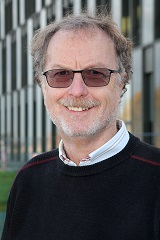
\includegraphics[angle=0,scale=0.6]{Bilder/Hermann.jpg}}
\noindent\textbf{Prof. Dr. rer. pol. Hermann-Josef Kruse}\\
Fachhochschule Bielefeld\\
Fachbereich Ingenieurwissenschaften und Mathematik\\
\href{mailto:hkruse@fh-bielefeld.de}{hkruse@fh-bielefeld.de}
\\ \\
\textbf{Fachgebiete:} Wirtschaftsmathematik, Operations Research
\\ \\
Seit 1995 als Professor für Wirtschaftsmathematik (insbesondere Operations Research) an der Fachhochschule Bielefeld tätig und lehrt dort im Bachelor-Studiengang \textit{Angewandte Mathematik} und im Master-Studiengang \textit{Optimierung \& Simulation} des Fachbereichs \textit{Ingenieurwissenschaften \& Mathematik}. Gründungsmitglied des Forschungsschwerpunktes \textit{Angewandte Mathematische Modellierung \& Optimierung} (FSP AMMO) der FH Bielefeld. F\&E-Projekte im Bereich der Optimierung und Simulation diskreter Systeme zur Entscheidungsunterstützung bei betrieblichen Problemstellungen.

\subsection*{Kontaktdaten}
\noindent\textbf{Prof. Dr. Hermann-Josef Kruse}\\
Fachhochschule Bielefeld\\
Fachbereich Ingenieurwissenschaften und Mathematik\\
Interaktion 1\\
33619 Bielefeld\\
Telefon +49.521.106-7411\\
Telefax +49.521.106-7176\\
\href{mailto:hkruse@fh-bielefeld.de}{hkruse@fh-bielefeld.de}\\
Raum D 229\\

\end{document}


